% -*- TeX:SI -*-
% slovene sub-mode for spell check
%%%%%%%%%%%%%%%%%%%%%%%%%%%%%%%%%%%%%%%%%%%%%%%%%%%%%%%%%%%%%%%%%%%%%%%%%%%%%%%%%%%%%%%%%%%%%%%%%%%%%%%%%%%%%%%%%%%%%%%%
% Magistrsko delo - Kristjan Šoln
%%%%%%%%%%%%%%%%%%%%%%%%%%%%%%%%%%%%%%%%%%%%%%%%%%%%%%%%%%%%%%%%%%%%%%%%%%%%%%%%%%%%%%%%%%%%%%%%%%%%%%%%%%%%%%%%%%%%%%%%
\documentclass[a4paper,twoside,openright,12pt,slovene]{book}
\usepackage[pdftex]{UNI-LJ-FE-Diploma} % stil zaključnega dela UL FE
\usepackage[utf8]{inputenc} % predloga uporablja standardno kodiranje Unicode UTF-8, ki podpira šumnike
\usepackage[greek,english,slovene]{babel} % seznam uporabljenih jezikov (zadnji na seznamu je primarni)

% PDF/A %%%%%%%%%%%%%%%%%%%%%%%%%%%%%%%%%%%%%%%%%%%%%%%%%%%%%%%%%%%%%%%%%%%%%%%%%%%%%%%%%%%%%%%%%%%%%%%%%%%%%%%%%%%%%%%%
% Več o PDF/A v LaTeX-u: https://www.mathstat.dal.ca/~selinger/pdfa/
\usepackage{filecontents}
\begin{filecontents*}{\jobname.xmpdata}
    \Title{Razpoznava sestavin hrane na robnih napravah z uporabo lahkih modelov globokega učenja} % Mora biti enak kot je v prijavi teme!
    \Author{Kristjan Šoln} % Mora biti enak kot na naslovnici!
\end{filecontents*}
\usepackage[a-1b]{pdfx}
%%%%%%%%%%%%%%%%%%%%%%%%%%%%%%%%%%%%%%%%%%%%%%%%%%%%%%%%%%%%%%%%%%%%%%%%%%%%%%%%%%%%%%%%%%%%%%%%%%%%%%%%%%%%%%%%%%%%%%%%

% LaTeX PAKETI %%%%%%%%%%%%%%%%%%%%%%%%%%%%%%%%%%%%%%%%%%%%%%%%%%%%%%%%%%%%%%%%%%%%%%%%%%%%%%%%%%%%%%%%%%%%%%%%%%%%%%%%%
% Kompakten pregled LaTeX ukazov je dostopen na https://en.wikibooks.org/wiki/Category:Book:LaTeX
% Navodila posameznih uporabljenih paketov so dostopna na https://www.ctan.org

% Dodatni simboli
\usepackage{textcomp}                               % dodatni simboli (kot npr. €)
\usepackage{gensymb}                                % dodatni simboli \de­gree, \cel­sius, \pert­hou­sand, \mi­cro, \ohm
\newcommand{\uppi}{\textrm{\greektext p\latintext}} % velika grška črka P z \uppi, alternativa simbolu \Pi
\newcommand{\etal}{\textit{et al.}} % Et al command
\usepackage{csquotes}

% Osnovno oblikovanje
\hypersetup{unicode,hidelinks,breaklinks,hyperindex} % dodatne možnosti hiperpovezav
\usepackage[normalem]{ulem}                          % podčrtavanje in prečrtavanje teksta
\usepackage{float}                                   % dodatne možnosti oblikovanja objektov
\usepackage{enumitem}                                % dodatne možnosti oblikovanja seznamov
\usepackage{amsfonts} % omogoča uporabo \mathbb
\usepackage{hyperref}

% Dodatno oblikovanje
%\zamaknirobsodihstrani{0mm} % dodatna prilagoditev levega roba sodih strani za dvostranski tisk
%\usepackage{dcolumn}        % poravnava po decimalnih mestih v tabelah
%\usepackage{longtable}      % večstranske tabele
%\usepackage{caption}        % dodatne možnosti označevanja objektov
\usepackage{rotating}       % vrtenje objektov, strani, ipd.
\usepackage{booktabs}

% Matematična orodja
\usepackage{mathtools} % http://mirrors.ctan.org/macros/LaTeX/contrib/mathtools/mathtools.pdf
\usepackage{bm}        % ukaz za odebeljeni tisk \bm v matematičnih okoljih
%\usepackage{cancel}   % ukaz za prečrtavanje \cancel v matematičnih okoljih
\usepackage{multirow}

% Grafična orodja
\usepackage{graphicx}                 % vključevanje bitnih slik z ukazom \includegraphics
\usepackage{grffile}                  % podpora presledkom pri ukazu \includegraphics
\usepackage{tikz}                    % paket TikZ za risanje (npr. blokovnih shem, diagramov poteka, itd.)
\usetikzlibrary{calc,shapes,arrows}  % dodatne možnosti paketa TikZ
\usepackage{tikzscale}               % skaliranje risb
%\usepackage[smartlabels]{circuitikz} % risanje shem vezij
\usepackage{pgfplots}                % paket PGFPlots za risanje grafov, tudi iz CSV in podobnih datotek
\usepgfplotslibrary{polar,external,groupplots}  % dodatne možnosti paketa PGFPlots
%\usepackage{tikz-3dplot}             % 3D risanje
% Primeri: http://texample.net , http://pgfplots.net/tikz/examples , http://pgfplots.sourceforge.net/gallery.html

\pgfplotsset{compat=newest}
\usepackage{booktabs}

% Rendranje grafov lahko precej poveča compile time. Te opcije omogočajo izvoz figure in uporabo tako shranjene PDF datoteke.
%\tikzexternalize[prefix=externalized/]

% Vključevanje datotek
\usepackage{pdfpages} % vključevanje PDF datotek z ukazom \includegraphics
\usepackage{epstopdf} % vključevanje EPS datotek z ukazom \includegraphics
\usepackage{listings} % orodja za izpisovanje programske kode
\lstset{              % nastavitve orodja za izpisovanje programske kode
    basicstyle=\ttfamily\footnotesize,
    breaklines=true,
    numbers=left,
    numberstyle=\scriptsize,
    keywordstyle=\color{blue},
    commentstyle=\color{unilj},
    stringstyle=\color{olive},
}


% Force no hyphenation or specific hypenation points
% TODO: Debug this
% TODO: verify whether this still works with stripped trailing numbers
\hyphenation{GoogleNet CNN}
\hyphenation{TinyML}
\hyphenation{AlexNet}
%\hyphenation{EfficientNetB7}
%\hyphenation{EfficientNetB0}
\hyphenation{EfficientNet}
\hyphenation{FOMO}
\hyphenation{SqueezeNet}
%\hyphenation{MobileNetV1}
%\hyphenation{MobileNetV2}
%\hyphenation{FoodSeg103}
\hyphenation{FastSAM}
\hyphenation{MobileSAM}

% Force no hypenation for all-uppercase words
\uchyph=0

%%%%%%%%%%%%%%%%%%%%%%%%%%%%%%%%%%%%%%%%%%%%%%%%%%%%%%%%%%%%%%%%%%%%%%%%%%%%%%%%%%%%%%%%%%%%%%%%%%%%%%%%%%%%%%%%%%%%%%%%

% DEKLARACIJE %%%%%%%%%%%%%%%%%%%%%%%%%%%%%%%%%%%%%%%%%%%%%%%%%%%%%%%%%%%%%%%%%%%%%%%%%%%%%%%%%%%%%%%%%%%%%%%%%%%%%%%%%%
\naslov{Razpoznava sestavin hrane na robnih napravah z uporabo lahkih modelov globokega učenja} % Mora biti enak kot je v prijavi teme!
\avtor{Kristjan Šoln} % Mora se ujemati s \Title pri metapodatkih PDF/A!
\mentor{izr. prof. dr. Janez Perš}
\somentor{asist. dr. Gregor Koporec}
\date{Ljubljana, \the\year}
\univerza{Univerza v Ljubljani}
\definecolor{unilj}{cmyk}{0.00, 0.94, 0.94, 0.06} % barva Univerze v Ljubljani

% Potrebno je paziti, da je izbrana prava kombinacija tipa dela in sodelujočih fakultet glede na študijski program!
\delo{Magistrsko delo\\~\\Magistrski študijski program druge stopnje Elektrotehnika}
\fakulteta{Fakulteta za elektrotehniko}
%%%%%%%%%%%%%%%%%%%%%%%%%%%%%%%%%%%%%%%%%%%%%%%%%%%%%%%%%%%%%%%%%%%%%%%%%%%%%%%%%%%%%%%%%%%%%%%%%%%%%%%%%%%%%%%%%%%%%%%%

% DOKUMENT %%%%%%%%%%%%%%%%%%%%%%%%%%%%%%%%%%%%%%%%%%%%%%%%%%%%%%%%%%%%%%%%%%%%%%%%%%%%%%%%%%%%%%%%%%%%%%%%%%%%%%%%%%%%%
\begin{document}
\frontmatter

\selectlanguage{slovene}

%******************************* NASLOVNICA ************************************
\maketitle

%******************************* ZAHVALA ***************************************
\zahvala
% TODO: Dodaj
V zahvali se kandidat lahko zahvali mentorju in poimensko tudi vsem sodelavcem in prijateljem, ki so pomagali in prispevali pri delu v laboratoriju, na računalniku, v delavnici, pri tehnični izdelavi dela ali drugje.

%******************************* POVZETEK IN KLJUČNE BESEDE ********************
\povzetek
% TODO: Dodaj
V tem dokumentu so predstavljena navodila za izdelavo zaključnega dela na FAKULTETI za elektrotehniko v Ljubljani. Zaključno delo predstavlja diplomsko delo na prvi in magistrsko delo na drugi stopnji izobraževalnega programa.

V povzetku v slovenščini in v angleščini kandidat navede glavne rezultate dela, zato naj povzetek seznani bralca z jedrom dela na način, ki je običajen za pisanje krajših člankov ali referatov. Obseg povzetka je za Repozitorij Univerze v Ljubljani omejen na 20.000 znakov.

Povzetek se prične z opisom in definicijo problema. Nadaljuje se z opisom uporabljenih metod in postopkov, ki so privedli do rešitve. Na koncu so opisani rezultati dela in glavni zaključki, ki iz rezultatov izhajajo.

Za povzetkom se na isti strani navede še ključne besede.

\kljucnebesede
% TODO: Dodaj
beseda1, beseda2, ...

\selectlanguage{english}

%******************************* ABSTRACT AND KEYWORDS *************************

\abstract
% TODO: Dodaj
The thesis addresses...

\keywords
% TODO: Dodaj
word1, word2, ...

\selectlanguage{slovene}

%******************************* KAZALO ****************************************
\tableofcontents

%******************************* SEZNAM SLIK, SEZNAM TABEL *********************
% TODO: Besedilo v vseh seznamih mora biti kratko, ne celotno besedilo pod sliko.
\seznamslik

\seznamtabel
% TODO: Dodaj

%******************************* SEZNAM SIMBOLOV *******************************
%\seznamsimbolov
%V pričujočem zaključnem delu so uporabljene naslednje veličine in simboli:
%
%\begin{center}
%    \begin{tabular}{*{4}{l}} \hline
%        \multicolumn{2}{c}{\bf{Veličina / oznaka}}           & \multicolumn{2}{c}{\bf{Enota}} \\ \hline
%        Ime                & Simbol                          & Ime      & Simbol              \\ \hline
%        čas                & $t$                             & sekunda  & s                   \\
%        frekvenca          & $f$                             & Hertz    & Hz                  \\
%        tlak               & $p$                             & Pascal   & Pa                  \\
%        sila vzgona        & $\textbf{\textit{F}}_\text{vz}$ & Newton   & N                   \\
%        gostota            & $\rho$                          & -        & kg/m$^3$            \\
%        masa               & $m$                             & kilogram & kg                  \\
%        vhodna napestost   & $U_\text{vh}$                   & volt     & V                   \\
%        Jacobijeva matrika & $\mathbf{J}$                    & -        & -                   \\ \hline
%    \end{tabular}
%\end{center}
%
%Pri čimer so vektorji in matrike zapisani s poudarjeno pisavo. Natančnejši pomen simbolov ter njihovih indeksov je razviden iz ustreznih slik ali pa je pojasnjen v spremljajočem besedilu, kjer je simbol uporabljen.

\seznamkratic

V pričujočem zaključnem delu so uporabljene naslednje kratice:

% TODO: Konsistentno uporabljaj isti stil tabel skozi celoten dokument
\begin{center}
    \begin{tabular}{c c}
        \toprule
        \textbf{Kratica} & \textbf{Pomen} \\
        \midrule
        SVM     & Metoda podpornih vektorjev (angl. Support Vector Machine) \\
        CNN     & Konvolucijske nevronske mreže (angl. Convolutional Neural Networks) \\ 
        DNN     & Globoke nevronske mreže (angl. Deep Neural Networks) \\
        SOTA    & Vodilni pristop (angl. State of the Art) \\
        PTQ     & Kvantizacija po učenju (angl. Post-Training Quantization) \\
        QAT     & Ozaveščeno učenje (angl. Quantization-Aware Training) \\
        IoU     & Jaccardov indeks oz. presečišče nad unijo (angl. Intersection over Union) \\
        mIoU    & Srednji Jaccardov indeks (angl. Mean Intersection over Union) \\
        \bottomrule
    \end{tabular}
\end{center}

\mainmatter

%******************************* UVOD ******************************************
\chapter{Uvod} \label{sct:uvod}


    % Zakaj je hrana pomembna
    % Tekom zgodovine je bila glavna skrb povezana s hrano predvsem količina; priprava in uživanje hrane sta vsakodnevni dejavnosti in del kulture, kjer iz osnovnih sestavin z različnimi postopki ustvarimo jedi. V preteklosti je bil temeljni poudarek, da postopki hrano naredijo lažje prebavljivo in varno za uživanje; danes, v obdobju izobilja, pa se težišče pogosteje premakne k okusu, konsistenci, ponovljivosti in preprostosti priprave. V tem okviru se vse pogosteje pojavlja tudi vidik zdrave priprave: izbira tehnik, ki ohranijo hranila in zmanjšajo nepotrebne dodatke.

    % - peka/priprava hrane na splošno
    Kuhanje je staro skoraj toliko kot človeška civilizacija - po arheoloških ocenah so zgodnji ljudje že pred približno 1,5 milijona let obvladali rabo ognja in ga začeli uporabljati pri pripravi hrane~\cite{src:myhrvold_cooking_2025}.
    %- zakaj je pomembna - mogoče s tem naredimo hrano lažje prebavljivo in bolj varno?
    Toplotna obdelava živil praviloma poveča njihovo prebavljivost in s tem olajša izrabo energije ter nekaterih hranil. Tako je kuhanje našim zgodnjim prednikom omogočilo izkoriščanje širšega nabora prehranskih virov in iz njih pridobiti več hranilne vrednosti~\cite{src:myhrvold_cooking_2025}.
    Živila kot mleko, govedina in jajca se pred uživanjem toplotno obdelajo, da se uničijo patogeni mikroorganizmi in izboljša okus, tekstura in podobno. Tehnološki postopki predelave spremenijo mikrostrukturo živil, bogatih z beljakovinami, s čimer spremenijo postopek prebave in absorpcije beljakovin v želodcu in tankem črevesu~\cite{src:Loveday_2023}.

    % Povezava z zdravjem in okoljem, avtomatizacijo
    Prehrana močno vpliva na zdravje, hkrati pa je pomemben faktor za zmanjšanje vpliva na okolje~\cite{src:eat2019food}.
    % Povezava s tehnologijo.
    Pametni kuhinjski aparati lahko optimizirajo našo prehrano in omogočijo večjo natančnost ter ponovljivost pri kuhanju, medtem ko pametni hladilniki z upravljanjem zalog zmanjšajo količino zavržene hrane~\cite{src:GOLSHANY2025116557}. Nekatere raziskave kažejo, da lahko pametne kuhinje prinesejo tudi do 15~\% prihranka električne energije.

    % Zakaj je razpoznavanje hrane pomembno (zdravje debelost, ostalo zdravje, tut ostali izdelki kot kuhinjski aparati)
    Nove tehnologije – zlasti računalniški vid na napravah z omejenimi viri – lahko proces priprave hrane standardizirajo in olajšajo: zmanjšajo napake, skrajšajo čas ter razbremenijo uporabnika pri načrtovanju in izvedbi korakov. Že zgodnji poskusi nadzora peke so vključevali optične sisteme z obdelavo slik v pečici za spremljanje vizualnih značilnosti (barvni ton, teksturo, obliko) in s tem postavili temelje za samodejno vodenje procesa~\cite{src:paquet2012monitoring}.V zadnjih letih so se metode globokega učenja uveljavile tudi na področju razpoznave jedi in ocenjevanja količin, kar je spodbudilo razvoj aplikacij, ki proces priprave poenostavijo ali deloma avtomatizirajo~\cite{src:SEDEJ_2023, src:Nikodinovska_2024}.
    Razpoznava jedi je tako ključen gradnik, s katerim sistemom omogočimo, da v realnem času določijo, katera jed je prisotna na sliki, na tej osnovi prilagodijo naslednje korake in tako naredijo pripravo bolj zanesljivo in enostavno.

    % Zakaj je razpoznavanje sestavin hrane (ne samo celih jedi) pomembno
    Identifikacija jedi je v literaturi precej pogosto obravnavana naloga~\cite{src:vlachopoulou2023food, src:mohanty2022food, src:bolanos2017food, src:hassannejad2016food, src:martinel2018wide, src:tan2019efficientnet} na raznih podatkovnih zbirkah~\cite{src:bossard2014food, src:matsuda2012recognition, src:kawano2014automatic, src:chen2016deep}. Pri tem večina pristopov tipično predpostavlja zaprt, vnaprej določen seznam jedi. Takšna predpostavka pogosto vodi v slabšo fleksibilnost sistema, saj brez dodatnega učenja težko spreminjamo izbran nabor jedi.
    Nasprotno pa razpoznavanje samih sestavin omogoči, da tip jedi določimo na podlagi zaznanih komponent: nove jedi lahko dodajamo kot kombinacije sestavin (npr. z enostavno preslikavo med kombinacijami in jedmi), brez širjenja podatkovne zbirke ali ponovnega učenja modela.
    S takim pristopom bolje prenašamo visoko vizualno varianco in omogočamo razpoznavanje kompleksnih jedi z več komponentami, kjer se izgled med primeri močno razlikuje.
    S tem hkrati bistveno zmanjšamo prostor label, saj lahko iz manjšega nabora sestavin tvorimo veliko število jedi~\cite{src:bolanos2017food}.
    Zato je pristop s sestavinami bolj univerzalen od neposredne klasifikacije jedi, še posebej ko moramo sistem enostavno širiti in prilagajati.

    % Novejši pristopi se tipično lotijo segmentacije sestavin hrane
    Raziskovalci se danes razpoznavanja sestavin pogosto lotijo kot segmentacijski problem~\cite{src:wu2021large, src:lan2023foodsam, src:bolanos2016simultaneous, src:pfisterer2019segmentation, src:poply2021refined}. Pri tem pogosto uporabijo zbirke, kot je FoodSeg103~\cite{src:wu2021large}.
    % TODO: Pikselno natančne maske - prevod
    Segmentacija (semantična ali instančna) deluje na podlagi pikselno natančnih mask, s čimer lahko dosežemo tudi ocenjevanje količin ter hranilnih vrednosti. Pripadajoče arhitekture so načeloma računsko in pomnilniško zahtevne, zato jih težje uporabljamo na napravah z omejenimi viri.

    % Primerjava izvajanja v oblaku in na robnih napravah
    V kolikor ciljna naprava ni dovolj zmogljiva za izvajanje modela, je pogosta rešitev izvajanje modela v oblaku. S tem zagotovimo ustrezno strojno opremo za izvajanje modela, vendar hkrati vnesemo dodatne probleme v povezavi z latenco, stroški, povezljivostjo naprav ter zasebnostjo. Trend v praksi je zato optimizacija in izvajanje neposredno na t.i. robnih napravah~\cite{src:abadade2023comprehensive}.
    % Kaj je robna naprava
    Robna naprava (angl. \textit{edge device}) je lokalna strojna enota na robu omrežja~-~od naprav Raspberry Pi in pametnih telefonov vse do mikrokrmilnikov~-~ki podatke praviloma zajame in vsaj del obdelave izvede lokalno~\cite{src:abadade2023comprehensive, src:moosmann2024ultra_tinyissimoyolo, src:boyle2024dsort, src:lin2021memory, src:hymel2022edgeimpulse}. Za robne naprave z omejeno zmogljivostjo to pomeni iskanje kompromisov med natančnostjo in kompleksnostjo algoritmov, dobro pa je premisliti tudi, če lahko zahtevne algoritme, kot recimo segmentacijski algoritmi, nadomestimo s preprostejšimi pristopi.

    % PROBLEMATIKA NA TEM PODROČJU

    % Opredeli problem na tem področju - segmentacijski algoritmi so računsko zahtevni in robne naprave imajo določene omejitve, in ker je razpoznavanje sestavin je ekstra zahtevno področje.
    % Omejitve in izzivi
    Zastavljen problem razpoznavanja sestavin hrane je zahteven zaradi odprtosti okolja, tipične neenakomerne porazdelitve razredov v podatkovnih zbirkah sestavin, prekrivanj objektov na sliki, visoke znotrajrazredne variabilnosti ter nizke medrazredne variabilnosti~\cite{src:wu2021large, src:bossard2014food}.
    Problem dodatno otežuje kompleksnost segmentacijskih algoritmov in omejitve strojne opreme. Izbrane platforme omejuje predvsem pomnilnik, ki je pogosto v rangu nekaj megabajtov ali celo kilobajtov. To neposredno določa največjo velikost modela, ki se še lahko izvaja na napravi. Dodatno omejitev predstavlja podpora izvajalnega okolja, saj ta za robne naprave načeloma podpirajo precej ožji nabor operacij.
    Navedene omejitve uporabo modelov na takšnih napravah bistveno otežijo, še posebej, če želimo ohraniti natančnost, primerljivo z oblačnimi modeli.
    % Glej Mohanty2021 D.5. Negative Results da vidis kak so pocasi zgubljali frnikule in kaj vse so probali, pa ni uspelo.

    % NAMEN TEGA DELA - segmentacija, ki bi delovala na robnih napravah?

    % TODO: Koporec pravi da sem sodi: najdimo pristop razpoznavanja sestavin s segmentacijskimi algoritmi, ki bo deloval na robnih napravah.
    % TODO: Restrukturiraj? - Na kaksen nacin, s kaksnimi nalogami, s kaksnimi opravili smo eksperimentalno preverili izvedljivost razpoznave sestavin
    Namen te naloge je, da eksperimentalno preverimo izvedljivost razpoznave sestavin hrane na izbranih robnih napravah z izbranim pristopom FOMO~\cite{src:announcingfomo}, pri čemer uporabimo podatkovno zbirko FoodSeg103~\cite{src:wu2021large}. Želeli smo izpeljati smernice za industrijsko rabo, kjer so ključne zahteve strojna oprema in robustnost v realnih pogojih. Problema smo se lotili kot razpoznave sestavin hrane, ki predstavlja osnovo za nadaljnje delo, z vizijo kot razpoznavo kompleksnih jedi na osnovi sestavin. Uporabili smo alternativen pristop razpoznave sestavin namesto klasičnih segmentacijskih modelov, da je izvedba na ciljni strojni opremi lažja. Izbran pristop smo ovrednotili na zbirki FoodSeg103~\cite{src:wu2021large} in analizirati njegove omejitve. Prikazati smo želeli vpliv priprave modela za izvajanje na robnih napravah, kar zajema predvsem vpliv kvantizacije na velikost in uspešnost modela. Preučili smo tudi potencialne poenostavitve podatkovne zbirke, da lahko problem zastavimo drugače (npr. kot detekcijski problem). Na koncu smo na podlagi ugotovitev oblikovali jasne smernice in predloge za nadaljnje delo.

    % Opisi svojo resitev
    % - FOMO
    % - FoodSeg103
    % - Analiza poenostavitev, kot detekcijski problem
    % - ?
    % Ne obravnavamo [npr. večmodalnih modelov z besedilom/recepti] zaradi [razlog], prav tako ne [npr. kompleksnih segmentacijskih arhitektur], ker [omejitve].

    % Omejitev strojne opreme in izbor platforme STM32
    Omejili smo se na naslednjo strojno opremo: kot platformo izberemo mikrokrmilnike~STM32, ki imajo pomnilnik in shranjevalni prostor omejen na do nekaj megabajtov. Četudi so te omejitve stroge, so drugi pokazali, da je sorodne modele možno uporabljati tudi na takšnih napravah~\cite{src:Nikodinovska_2024}. Pristop dodatno podpira orodje X-CUBE-AI za izvajanje modelov~\cite{src:stxcubeai-docs} ter nabor referenčnih modelov, dokumentiranih in pripravljenih za izvajanje na izbrani platformi~\cite{src:stm32modelzoo}.
    Zaradi strogih omejitev pomnilnika, računske moči in porabe energije moramo globoke modele primerno optimizirati, kar je danes aktivno področje raziskav in razvoja.
    V tem delu uporabimo model Faster Objects, More Objects (FOMO) platforme Edge Impulse~\cite{src:announcingfomo}, detekcijski pristop za mikrokrmilnike, ki se izogne klasični strukturi detektorjev in na izhodu ustvari grobo segmentacijsko masko. Slednja se običajno naknadno obdela (npr. z združevanjem/rojenjem), da na izhodu dobimo lokacije objektov.
    % TODO: Razširi. Povej prednosti in slabosti modela.

    % TODO: Tole verjetno paše kam drugam
    V kontekstu tega dela nas zanima prisotnost sestavin, zato smo postopek priredili tako, da smo informacijo o lokalizaciji opustili in gledali zgolj zadostno prisotnost sestavin na maski. Z eksperimenti smo ugotovili, da je model učinkovit na robnih napravah z omejeno zmogljivostjo, vendar se je izkazalo, da ima tudi določene slabosti. Med njih sodijo majhno receptivno polje in omejena kapaciteta modela, kar omeji končno uspešnost pristopa~\cite{src:boyle2024dsort}.

    % Kratek opis rezultatov
    Z izbrano rešitvijo smo dosegli zgolj omejene rezultate. Metoda FOMO je pomanjkljiva in ima težave predvsem z velikostjo receptivnega polja ter zahteva precej naknadne obdelave rezultatov. Težavo je predstavljala tudi odprta narava podatkovne zbirke in neugodna distribucija razredov, tipična za problematiko razpoznavanja sestavin hrane. Pristopi drugih avtorjev na podatkovni zbirki FoodSeg103~\cite{src:wu2021large} se večinoma ukvarjajo s semantično segmentacijo in ne ciljajo na izvajanje na mikrokrmilnikih, zaradi česar so njihove rešitve večinoma neprimerne za naš namen. Ovire, na katere smo naleteli tekom eksperimentov, kažejo, da je razpoznavanje sestavin hrane zahtevno področje, ki v mnogih pogledih še ni zadovoljivo rešeno.

    % Struktura dokumenta.
    Delo se začne s pregledom sorodnih del v poglavju~\ref{sct:sorodna-dela}. V poglavju~\ref{sct:metodologija} predstavimo teoretično ozadje izbranih pristopov ter podrobneje opišemo arhitekturo modela FOMO in teoretične osnove pristopov YOLOv11-seg in SAM. V poglavju~\ref{sct:eksperimenti-in-rezultati} opišemo uporabljeno podatkovno zbirko in izvedene eksperimente, v poglavju~\ref{sct:diskusija} pa komentiramo rezultate in iz njih izpeljemo smernice za nadaljnje delo. Delo zaključimo v poglavju~\ref{sct:zakljucek}, kjer povzamemo ključne ugotovitve.

\chapter{Sorodna dela} \label{sct:sorodna-dela}

    V tem poglavju predstavimo sorodna dela s področja razpoznavanja jedi ter izvajanja modelov globokega učenja na robnih napravah. Razpoznavanje jedi podrobneje obravnavamo v poglavju~\ref{sct:razpoznavanje-jedi-na-slikah}, kjer predstavimo zgodnje pristope razpoznavanja jedi, uveljavljene pristope globokega učenja, novejše večmodalne metode, ki upoštevajo dodatne informacije o sestavinah, ter naredimo pregled pristopov za klasifikacijo, detekcijo in segmentacijo jedi ter sestavin. Nato v poglavju~\ref{sct:izvajanje-na-robnih-napravah} podrobneje predstavimo pregled obstoječih pristopov, ki modele globokega učenja izvajajo na robnih napravah ter tam uporabljeno strojno opremo.

    \section{Razpoznavanje hrane iz slikovnih vzorcev} \label{sct:razpoznavanje-jedi-na-slikah}

        Med zgodnjimi pristopi k razpoznavanju jedi iz slik so prevladovale ročno izluščene značilnice, predvsem SIFT (angl. \emph{Scale-Invariant Feature Transform})~\cite{src:lowe2004sift}, HOG (histogram orientiranih gradientov)~\cite{src:dalal2005hog} in barvni histogrami~\cite{src:min2019survey}.
        V nekaterih zgodnjih delih~\cite{src:wang2003assessment, src:segnini1999low} so avtorji povprečili svetlosti slikovnih elementov na sivinskih slikah ter na tej osnovi določali lastnosti sira med peko in ocenjevali kakovost čipsa.
        V novejših pristopih avtorji pogosto uporabljajo metode globokega učenja, s katerimi dosegajo boljše rezultate~\cite{src:min2019survey, src:kagaya2014food, src:krizhevsky2012imagenet, src:hassannejad2016food, src:martinel2018wide}.
        Pristope za razpoznavanje hrane na slikah v grobem delimo na klasifikacijske in segmentacijske~\cite{src:konstantakopoulos2023review, src:min2019survey}. Klasifikacijski izvajajo enoznačno ali večznačno klasifikacijo jedi oziroma sestavin~\cite{src:martinel2018wide, src:tan2019efficientnet, src:bolanos2017food, src:fu2024recognizing}, segmentacijski pa lokalizirajo in razmejujejo posamezne komponente ter jih po potrebi tudi kategorizirajo~\cite{src:wu2021large, src:bolanos2016simultaneous, src:poply2021refined, src:konstantakopoulos2023review, src:javadi2024smart}.

        \subsection{Klasifikacija jedi}

            Med temeljne naloge razpoznavanja hrane sodi klasifikacija, pri kateri z metodami strojnega učenja iz slikovnih podatkov napovemo kategorijo jedi ali posameznih sestavin~\cite{src:min2019survey}.
            % Klasični pristopi, začetki
            V tradicionalnih klasifikacijski pristopih značilke tipično izluščimo ročno, nato pa jih uporabimo v razvrščevalniku~\cite{src:min2019survey}.
            % TODO: Prevedi superpiksle?
            V~\cite{src:bossard2014food} so avtorji uporabili metodo naključnega gozda~(angl. random forest)~\cite{src:breiman2001randomforest} ter metodo superpikslov~\cite{src:ren2003superpixels} za identifikacijo ključnih področij oz. komponent slike jedi. Značilke identificiranih komponent so nato razvrstili z metodo podpornih vektorjev (angl. support vector machine, SVM)~\cite{src:cortes1995svm} in tako določili tipa jedi.
            Podobno so v~\cite{src:yang2010food} avtorji na slikah jedi identificirali lokalne lastnosti slikovnih elementov in njihove soodvisnosti ter jih zajeli v histogramu. Tega so nato uporabili kot vektor značilk v razvrščevalniku SVM~\cite{src:cortes1995svm}.
            V~\cite{src:pouladzadeh2015cloud} so avtorji združili značilke na podlagi barve, teksture, velikosti in oblike, nato pa v oblaku z metodo SVM~\cite{src:cortes1995svm} razvrščali 30 vrst hrane in dosegli 94,5-odstotno natančnost. 

            % Deep learning era - začetki
            Z uporabo globokega učenja in konvolucijskih nevronskih mrež je prišlo do precejšnih izboljšav tudi na področju razpoznavanja hrane.
            % Kagaya 2014 - Among the first to try DNN on food datasets.
            V~\cite{src:kagaya2014food} so avtorji primerjali klasične pristope z metodami na podlagi konvolucijskih nevronskih mrež (angl. Convolutional Neural Networks, CNN)~\cite{src:krizhevsky2012imagenet} in s slednjimi dosegli veliko boljše rezultate. Navajajo še, da se je tako naučena mreža med klasifikacijo zanašala predvsem na barvo objektov na sliki.
            % Hassannejad 2016 [90] - Inception V3
            Hassannejad~\etal~\cite{src:hassannejad2016food} so model Inception~V3~\cite{src:szegedy2016rethinking} doučili na zbirkah UEC-Food100~\cite{src:matsuda2012recognition}, UEC-Food256~\cite{src:kawano2014automatic} in Food-101~\cite{src:bossard2014food}. Na posameznih zbirkah so dosegli natančnosti 81{,}5~\%, 76{,}2~\% ter 88{,}3~\%. Dobre rezultate so dosegli s precej manj parameteri kot konkurenca, vendar njihov pristop še vedno ni bil primeren za izvajanje na robnih napravah.
            % Matrinel 2018 - WISeR
            V~\cite{src:martinel2018wide} so avtorji predstavili arhitekturo WISeR, globoki model za klasifikacijo slik hrane, kjer so uporabili novo plast, namenjeno zaznavanju navpičnih struktur v jedeh, kjer se komponente prekrivajo in so naložene vertikalno. Njihov pristop je presegel obstoječe CNN-modele na zbirkah Food-101~\cite{src:bossard2014food} z več kot 90~\% natančnostjo. Kljub visoki natančnosti kompleksnost modela omejuje njegovo uporabnost na napravah z omejeno strojno opremo.
            % Tan 2019 [91] - EfficientNetB7 - among the best solutions to Food-101 according to the 2024 review
            Tan~\etal~\cite{src:tan2019efficientnet} so uvedli družino modelov EfficientNet, s katerim so dosegli zelo dobre rezultate na več podatkovnih zbirkah. Med drugim so na Food-101~\cite{src:bossard2014food} z EfficientNetB7 dosegli 93~\% natančnost.
            % TODO: Naslednji dve povedi mogoče prestavi v odsek kjer govoriš o izvajanju na robnih napravah.
            % VijayaKumari 2022 [80] - EfficientNetB0
            Nekateri avtorji so ocenjevali tudi druge modele iz te družine. V~\cite{src:vijayakumari2022food} so z EfficientNetB0 na Food-101 dosegli 80~\% natančnost. Izbrana različica uporablja zgolj 11 milijonov parametrov, kar omogoča izvajanje na precej širšem naboru strojne opreme.
            % Moumane 2023 - MobileNetV2 on mobile phone
            V~\cite{src:moumane2023food} so avtorji  uporabili MobileNetV2~\cite{src:sandler2018mobilenetv2} za klasifikacijo zbirke Food-101~\cite{src:bossard2014food}. Avtorji so izbran model implementirali v mobilni aplikaciji za izvajanje na pametnih telefonih.
            % Izbran model je zaradi svoje učinkovitosti primeren tudi za izvajanje na robnih napravah.
            % Ta članek izgleda precej nekvaliteten, vendar je eden redkih, ki poskuša uporabiti MobileNetV2 na Food-101 oz. ostalih food-related datasetih. Ne zaupam         % Prav detekcija/klasifikacija sestavin
            Bolanos~\etal se v delu~\cite{src:bolanos2017food} namesto klasifikacije samih jedi lotijo klasifikacije sestavin, prisotnih na sliki. Uporabili so zbirko Food-101~\cite{src:bossard2014food}, ki sicer vsebuje oznake jedi, a so jih ročno zamenjali z oznakami sestavin. Uporabili so standarden večznačen pristop razvrščanja z InceptionV3~\cite{src:szegedy2016rethinking} in ResNet50~\cite{src:he2016deep} ter dosegli do 80~\% natančnosti po metriki razvrščanja F1. % večznačen - multi-label
            Preverili so tudi sposobnost generalizacije modela na nove slike jedi, kjer so na modificirani zbirki Recipes5k~\cite{src:bolanos2017food} dosegli do 47~\% po metriki F1. Slabost njihovega pristopa je, da so vsakemu receptu pripisali množico sestavin, ne glede na to, ali je dana sestavina vidna ali ne.
            V~\cite{src:fu2024recognizing} so avtorji raziskovali uporabo principa drsečega okna (angl. \textit{sliding window}). Klasifikacijo izrezanih delov slike so izvajali s prilagojenim EfficientNetB0~\cite{src:tan2019efficientnet}. Tako so v končnem sistemu z razvrščevalnikom za vsak izrezek predvideli en tip sestavine, nato pa rezultate vseh izrezkov združili po principu glasovanja. Na tak način so rekonstruirali seznam vseh prisotnih sestavin. Učenje so avtorji v~\cite{src:fu2024recognizing} sicer izvajali na zasebni podatkovni zbirki, vendar so evalvacijo izvedli tudi na poenostavljeni zbirki FoodSeg103~\cite{src:wu2021large}. Poenostavitev so izvedli tako, da so med testiranjem upoštevali rezultate le za 35 razredov, ki so se prekrivali z njihovo zasebno podatkovno zbirko.
            % (kjer so dosegli do 53~\% po metriki mAcc) - rezultat ni relevanten, ker ne vem točno kaj so delali z metriko, imajo malo citatov, in uporabljajo poenostavljeno/spremenjeno zbirko.

            % Upoštevanje informacije o sestavinah
            Že v zgodnjih pristopih~\cite{src:bossard2014food} so si raziskovalci pri razpoznavi slik pomagali s t.i. komponentami, t.j. lokalnimi regijami slike podobne teksture in barve. % To malo spominja na sestavine
            % Maybe cite Mao2021, also see the Multiple Food recognition section in related work
            % Maybe cite Matsuda, Y., Hoashi, H., Yanai, K.: Recognition of multiple-food images by detecting candidate regions. (2012)
            % See Wang2022 related work
            %Wu et al.~\cite{src:wu2021large} proposed a food image segmentation framework, which consists of two modules: Recipe Learning Module (ReLeM) and Image Segmentation module. Specially, ReLeM incorporates recipe information and integrates recipe embedding with the visual representation of a food image to enhance the visual representation of an ingredient.
            % Salvador 2017 - Recipe1M
            Salvador~\etal~\cite{src:salvador2017learning} so predstavili podatkovno zbirko Recipe1M in večmodalen pristop k določanju jedi.
            V njihovem pristopu so najprej implicitno predvideli sestavine, na podlagi tega pa določili ime jedi oziroma recepta na sliki. Razpoznavanje sestavin je bil tu pomemben vmesni korak za razpoznavo same jedi.
            V delu~\cite{src:min2019ingredient} so avtorji predstavili IG-CMAN (angl. Ingredient-Guided Cascaded Multi-Attention Network), kjer so uporabili t.i. Spatial Transformer model~\cite{src:jaderberg2015spatialtransformer} % TODO: Prevod za spatial transformer?
            ter LSTM (angl. Long Short-term Memory)~\cite{src:hochreiter1997lstm} za šibko nadzorovano lokalizacijo regij na sliki~\cite{src:wang2017multi}. Čeprav je model izvajal razvrščanje na nivoju jedi, je med učenjem uporabljal tudi informacijo o sestavinah jedi na sliki. Avtorji so za izbrano metodo navedli 90~\% Top-1 natančnost na zbirki Food-101~\cite{src:bossard2014food}.
            % Multi-label Image Recognition by Recurrently Discovering Attentional Regions - tu se grejo tut nek attention, ampak klasifikacija. Ni z jedmi. Je direktni inspiration za min2019ingredient, ampak se se zmeraj razlikujejo.
            % Food detection with YOLO: "Radeva, P.: Grab, pay, and eat: Semantic food detection for smart restaurants."
            % Relevant for FOMO: "MCUNetV2: Memory-Efficient Patch-based Inference for Tiny Deep Learning"
            Poleg večmodalnosti so se v nekaterih pristopih pojavili tudi VT (angl. Vision Transformer)~\cite{src:dosovitskiy2020image} modeli. Liu~\etal~\cite{src:liu2024convolution} so predstavili dvodelno arhitekturo, kjer so na podlagi slike predvideli kategorijo hrane in sestavine, prisotne na sliki. Pri tem so uporabljali prilagojen VT model za pridobivanje značilk na več nivojih, nato pa so s prilagojenim modulom z adaptivno pozornostjo poskrbeli za deljenje informacij med razvrščevalniki. Pristop je dosegel 92~\% in 93~\% natančnosti na zbirkah \mbox{Food-101}~\cite{src:bossard2014food} in \mbox{VireoFood-172}~\cite{src:chen2016deep}.

        % Weakly supervised ingredient segmentation/detection
            Nekateri pristopi so uporabili tudi t. i. šibko nadzorovano učenje, s katerim so se poskusili izogniti potrebi po segmentacijskih podatkovnih zbirkah, saj so s tem pristopom potrebovali le informacijo o prisotnosti sestavine na sliki (t.i. anotacije na nivoju slike), pri čemer so še vedno skušali v model vključiti vizualne predstave sestavin~\cite{src:zhu2023new}.
            Vlachopoulou~\etal~\cite{src:vlachopoulou2023food} so tako uporabili šibko nadzorovane pristope iz sorodnih področij, med drugim iz medicine, za razpoznavo sestavin jedi: sliko so razbili v posamezne zaplate, za vsako zaplato so z ResNet-34~\cite{src:he2016deep} izračunali značilnice, mehanizem za pozornost (angl. attention mechanism)~\cite{src:ilse2018attention} pa jih je utežil in združil. Tako združen predstavitveni vektor so nato peljali v razvrščevalnik. Modele so učili na FoodSeg101~\cite{src:bossard2014food}, vendar so zbirko močno poenostavili. Poenostavljena zbirka je imela zgolj dve kategoriji (meso in pekovski izdelki), anotacije pa so pretvorili iz nivoja slikovnih elementov na nivo slike. Avtorji~\cite{src:vlachopoulou2023food} so za vsako kategorijo naučili povsem ločen model, da so se čim bolj izognili medsebojnemu vplivu sestavin. Dosegli so uspešnost 71{,}3~\% po metriki razvrščanja F1, vendar njihovi rezultati niso neposredno primerljivi z drugimi deli zaradi omenjenih poenostavitev podatkovne zbirke.
            Sorodno so Zhu~\etal~\cite{src:zhu2023new} predstavili arhitekturo AttNet. Posamezne sestavine so razdelili v štiri nivoje kategorij, AttNet pa je za dano sliko poskušal napovedati vse štiri nivoje. Tako kot v prejšnjem pristopu~\cite{src:vlachopoulou2023food} so tudi tu za vsako sestavino naučili lasten model. Kasneje so v~\cite{src:zhu2023new} uporabili značilke iz konvolucijskih plasti v mreži in s filtri ter rojenjem izrazili približek segmentacijske maske. Model se ni neposredno učil ločevanja meje med sestavinami, le ločevanje globalnega videza posamezne sestavine. Ker so konvolucijske značilke lokalne, se je ista aktivacija pojavila točno tam, kjer so bili slikovni elementi te sestavine, kar je omogočilo kasnejšo rekonstrukcijo maske. S tako pridobljenimi segmentacijskimi maskami so poročali do 65{,}3~\% po metriki mIoU na FoodSeg103~\cite{src:wu2021large}. Njihovi rezultati, čeprav zelo dobri, niso bili neposredno primerljivi z drugimi metodami, saj so avtorji omenjeno zbirko modificirali - ozadje so zamenjali z modro barvo. %Slabosti te metode?

        \subsection{Segmentacija jedi}

            Za nekatere namene, kot na primer napovedovanje prehranske vrednosti jedi, sama klasifikacija ni dovolj. V primerjavi z običajno klasifikacijo segmentacija poda bistveno več informacij o vsebini slike, vendar je praviloma tudi zahtevnejša naloga, saj zahteva napoved oznak na nivoju slikovnih elementov~\cite{src:konstantakopoulos2023review, src:minaee2021image}. Razpoznavanje jedi oziroma sestavin predstavlja dodatno oviro, ker je za to področje značilna visoka varianca znotraj razredov in nizka varianca med razredi~\cite{src:wu2021large}. Namen segmentacije jedi je lokalizacija jedi oziroma posameznih območij na sliki, njihovo ločevanje od preostalih območij oziroma ozadja ter pripisovanje kategorije izločenemu območju~\cite{src:konstantakopoulos2023review}.
            Med bistvenimi podatkovnimi zbirkami, ki se pogosto uporabljajo v tovrstnih pristopih, so FoodSeg103~\cite{src:wu2021large}, UECFoodPix~\cite{src:ege2019new} ter UECFoodPix Complete~\cite{src:okamoto2021uec}.

            % Konstantakopoulos~\textit{et al.}~\cite{src:konstantakopoulos2023review} ločijo segmentacijske metode na pol-avtomatske, avtomatske s tradicionalnimi pristopi za ekstrakcijo značilk ter avtomatske z globokim učenjem. 
            Tradicionalni segmentacijski pristopi so uporabljali teksturo, obliko ter ročno izpeljane značilke na podlagi barve za določanje področij~\cite{src:konstantakopoulos2023review}. 
            % Anthimopoulos 2013 - early food segmentations
            Anthimopoulos~\etal~\cite{src:anthimopoulos2013segmentation} so uporabili pet-koračni algoritem na podlagi značilk, izpeljanih iz barve, združevanja regij ter detekcije krožnika.
            % Pouladzadeh 2014 - neka tradicionalna segmentacija 
            Pouladzadeh~\etal~\cite{src:pouladzadeh2014using} so uporabili metodo reza v grafu (angl. graph cut)~\cite{src:boykov2001interactive-graphcut} za določanje regij, te pa so razvrstili z metodo SVM~\cite{src:cortes1995svm}.

            % Deep learning segmentation - intro
            Pristopi, ki uporabljajo globoko učenje, so dosegali bistveno boljše rezultate~\cite{src:minaee2021image}.
            % Bolanos 2016 - deep learning segmentacija
            Bolanos~\etal~\cite{src:bolanos2016simultaneous} so uporabili model GoogleNet~\cite{src:szegedy2015going-googlenet} in rezultate združili v sliko aktivacij (angl. heatmap), nato pa posamezne aktivacije še kategorizirali.
            % Shimoda 2020 - class activation mapping
            Shimoda~\etal~\cite{src:shimoda2020weakly} so predstavili šibko nadzorovano metodo za segmentacijo krožnika na sliki. Pri tem so iz barvne slike hrane najprej izpeljali psevdo-segmentacijsko masko, v kateri so bili slikovni elementi razvrščeni v kategorije \enquote{hrana}, \enquote{krožnik} ali \enquote{ozadje}, ter z njo učili model za segmentacijo krožnika. Ključni del pristopa je temeljil na preslikavi aktivacij razredov (angl. Class Activation Mapping, CAM)~\cite{src:zhou2016learning-cam}, ki se tipično uporablja za vizualizacijo diskriminativnih regij v CNN modelih; avtorji so iz razlike med CAM klasifikatorja kategorije jedi in CAM binarnega klasifikatorja ocenili področje krožnika. V nadaljevanju so tako pridobljeni model uporabili pri regularizaciji šibko nadzorovane semantične segmentacije hrane ter s tem izboljšali delovanje osnovnega pristopa. Na zbirki UEC-Food100~\cite{src:matsuda2012recognition} so metriko mIoU izboljšali za 5{,}7 odstotne točke in dosegli 55{,}4~\%.

            % Okamoto 2021 - DeepLabV3+, uvedli FoodPix Complete
            Okamoto~\etal~\cite{src:okamoto2021uec} so predstavili zbirko UEC FoodPix Complete in jo evalvirali z modelom DeepLab V3+~\cite{src:chen2017deeplab}. Dosegli so 55{,}5~\% po metriki mIoU.
            % Poply - something something instance segmentation
            Poply~\etal~\cite{src:poply2021refined} so semantično segmentacijo uporabili pri estimaciji prehranske vrednosti živil na krožniku. V grobem so posnemali instančno segmentacijo, saj so uporabili detekcijski model za določanje kandidatov v koraku segmentacije. V njihovem pristopu so uporabljali zasebno podatkovno zbirko.

            % Wu 2021 - ReLeM semantic segmentation (+ recipe embeddings)
            Wu~\etal~\cite{src:wu2021large} so objavili podatkovno zbirko FoodSeg103 za segmentacijo sestavin hrane v nenadzorovanem okolju ter predstavili večmodalni model ReLeM, ki je poleg slik uporabil tudi tekstovne recepte v obliki jezikovnih vektorjev. Z ReLeM so na FoodSeg103 dosegli do 43{,}2~\% mIoU in na isti zbirki ovrednotili še več obstoječih modelov (DeepLab V3~\cite{src:chen2017deeplab}, CCNet~\cite{src:huang2019ccnet}, FPN~\cite{src:kirillov2019panoptic} in SeTR~\cite{src:zheng2021rethinking}). Najboljši rezultat 43{,}2~\% mIoU so dosegli z modelom ReLeM. Rezultate na njihovi podatkovni zbirki so primerjali z rezultati na zbirki Cityscapes~\cite{src:cordts2016cityscapes}, kjer so dosegli bistveno boljše rezultate, kar je nakazalo na zahtevnost zbirke FoodSeg103.

            % Park 2021 - Mask RCNN, pretrained on synthetic data
            Park~\etal~\cite{src:park2021deep} so za segmentacijo učili model Mask R-CNN~\cite{src:he2017mask}, pri čemer so učenje osnovali na sintetičnih slikah, generiranih v orodju Blender. Model so nato doučili na resničnih posnetkih hrane iz lastne podatkovne zbirke.
            % Javadi 2024 - Mask R-CNN
            V~\cite{src:javadi2024smart} so predstavili pametni skener hrane, ki je z združevanjem senzorjev (kamera, tehtnica), modela Mask R-CNN za segmentacijo~\cite{src:he2017mask}, razvrščevalnika sestavin in globinske ocene omogočil samodejno določanje mase sestavin ter izračun hranilnih vrednosti. Zajem in predobdelava sta potekala na robni napravi, računsko zahtevnejši del obdelave pa v oblaku.
            % FoodSAM
            Lan~\etal~\cite{src:lan2023foodsam} so predstavili FoodSAM, ki je izhajal iz modelov Segment Anything (SAM)~\cite{src:kirillov2023segment}, namenjenih segmentaciji poljubnih objektov brez potrebe, da bi bili ti v učni množici (angl. zero-shot segmentation). Ker SAM sam po sebi praviloma vrne le segmentacijske maske brez razrednih oznak, so avtorji~\cite{src:lan2023foodsam} vzporedno dodali model SeTR~\cite{src:zheng2021rethinking}, ki je ustvaril grobe semantične maske z oznakami razredov. Rezultate obeh modelov so združili z mehanizmom glasovanja. Na FoodSeg103~\cite{src:wu2021large} so dosegli 46{,}4~\% mIoU na FoodSeg103 in 66{,}1~\% na UECFoodPix Complete~\cite{src:okamoto2021uec}.

    \section{Izvajanje na robnih napravah} \label{sct:izvajanje-na-robnih-napravah}

        % Early efforts
        Za področje izvajanja modelov na robnih napravah se pogosto uporablja termin TinyML~\cite{src:abadade2023comprehensive}. Med začetke teh pristopov na področju razpoznavanja hrane sodijo Kawano~~\etal~\cite{src:kawano2014foodcam} z modelom FoodCam-256, ki je bil pripravljen za izvajanje na mobilnih napravah, a je uporabljal tradicionalne pristope za klasifikacijo. Med pomembnejše pristope na tem področju sodita tudi SqueezeNet~\cite{src:iandola2016squeezenet} ter MobileNetV1~\cite{src:howard2017mobilenets}, ki sta v primerjavi z AlexNet~\cite{src:krizhevsky2012imagenet} ohranila oz. izboljšata natančnost, hkrati pa močno zmanjšala število parametrov.

        Izvedbe družine modelov MobileNet s SSD (angl. Single Shot Detection) ter FPN (angl. Feature Pyramid Network)~\cite{src:lin2017feature} omogočajo uporabo izbranih klasifikacijskih modelov tudi v kontekstu detekcije.
        % ST YOLO X
        Prav tako je možno nekatere bolj znane detekcijske modele, na primer YOLOX~\cite{src:ge2021yolox}, prirediti za izvajanje na mikrokrmilnikih~\cite{src:stm32modelzoo}.

        % FOMO
        Platforma Edge Impulse je predstavila model Faster Objects More Objects (FOMO)~\cite{src:fomodocs}, detekcijski model, namenjen izvajanju na mikrokrmilnikih. Sestavljen je iz začetnih plasti modela MobileNetV2~\cite{src:sandler2018mobilenetv2}, glava pa je zgolj konvolucijska plast, kar rezultira v mreži značilk oz. aktivacij za vsako kategorijo. To lahko interpretiramo tudi kot segmentacijsko masko z zelo nizko resolucijo. Na takšnem izhodu so avtorji izvedli algoritem rojenja, kjer je vsak roj predstavljal en objekt. Tako so izhod modela bila središča detektiranih rojev, kar je posnemalo izhode klasičnih detekcijskih modelov. Metoda je sicer zahtevala zelo malo pomnilnika in imela nizko računsko kompleksnost, slabosti pa so se skrivale v majhnem receptivnem polju (angl. low receptive field), združevanju sosednjih objektov tekom rojenja ter nižji kapaciteti modela~\cite{src:boyle2024dsort}.
        % Edge Impulse se ponaša predvsem s poenostavljanjem postopka zajema in obdelave podatkovne zbirke, učenja modela ter priprave modela za izvajanje na mikrokrmilnikih. Platforma omogoča popolnoma on line workflow, kompleksnost naloge pa zmanjšajo na račun fleksibilnosti pri načrtovanju. Načeloma je možno generirane skripte tudi urejati, kar omogoči boljši nadzor nad workflovom.
 
        % DSORT-MCU
        Problem združevanja objektov med rojenjem so deloma razrešili Boyle~\etal v DSORT-MCU~\cite{src:boyle2024dsort}, kjer so predstavili adaptivno deljenje slike. Sliko so najprej razdelili na prekrivajoče odseke, nato pa vsak odsek ločeno poslali skozi model FOMO~\cite{src:fomodocs}. Rezultate vseh so nato združili v končni izhod. S tem so izboljšali sposobnost modela FOMO~\cite{src:fomodocs} za štetje objektov.
        
        Čeprav obstaja precej pristopov za izvajanje na mikrokrmilnikih~\cite{src:abadade2023comprehensive}, je raziskav, ki njihovo uporabo obravnavajo v kontekstu razpoznavanja hrane, razmeroma malo~\cite{src:moumane2023food, src:Nikodinovska_2024}.
        % Klasifikacija
        Gutti~\etal~\cite{src:gutti2022real} so izdelali prototip za razvrščanje sadja in zelenjave na podlagi slik na ESP-32 mikrokrmilniku. Izvedli so primerjavo treh modelov - prilagojen CNN, MobileNetV1~\cite{src:howard2017mobilenets} ter MobileNetV2~\cite{src:sandler2018mobilenetv2}. Izmerili so hitrost inference do 51 ms in porabe do 66 kB pomnilnika. Lin~\etal~\cite{src:lin2020mcunet} so predstavili MCUNet, primeren za izvajanje na mikrokrmilnikih. Na ImageNet~\cite{src:russakovsky2015imagenet} so z njim dosegli 70{,}7~\% natančnost. Modela MobileNetV1~\cite{src:howard2017mobilenets} in MobileNetV2~\cite{src:sandler2018mobilenetv2} sta na isti zbirki dosegla 72{,}0~\% in 74{,}2~\% natančnost s 3{,}4 in 6{,}9 milijoni parametrov. 

        % Razpoznava hrane
        % Tipično avtorji ciljajo vsaj mobilne telefone.
        % Klasifikacija
        V STM32 Model Zoo~\cite{src:stm32modelzoo} na zbirki \mbox{Food-101}~\cite{src:bossard2014food} navajajo do 77{,}1~\% natančnost z MobileNetV1 ter do 80{,}38~\% natančnost z MobileNetV2. V realnosti je natančnost tipično nižja, saj je potrebno zmanjšati velikost modela glede na izbrano strojno opremo.
        Nikodinovska~\cite{src:Nikodinovska_2024} je na platformi STM32 implementirala model za klasifikacijo zapečenosti piškotov. 
        % Detekcija in segmentacija?
        Prednosti izvedbe na robnih napravah so jasne - hitrejši in preprostejši modeli, cenejša izvedba, naprav pa ni potrebno povezovati v oblak.

        % TODO: Po napisanem uvodu tu argumentiraj kaj ostalim pristopom manjka v primerjavi s tvojo idejo. Na objektiven način skritiziraj dela (uporabi to kar si že napisal). Lahko tut iz obeh podpoglavij v sorodnih delih. Nej bo to mini mini diskusija sorodnih del.

\chapter{Teoretično ozadje} \label{sct:teoreticno-ozadje}

    V tem poglavju na kratko predstavimo teoretični pregled pristopov, relevantnih v tem delu. V odsekih \ref{sct:teorija-klasifikacija} in \ref{sct:teorija-segmentacija} podamo osnovne pojme klasifikacije in segmentacije na podlagi slikovnih vzorcev, najprej splošno, nato pa še v kontekstu razpoznavanja jedi.
V odseku \ref{sct:teorija-robnenaprave} obravnavamo pristope izvajanje modelov globokega učenja na robnih napravah, naredimo pregled najpogostejših pristopov k optimizaciji ter predstavimo obstoječe programske rešitve in razvojna okolja, namenjena razvoju in uporabi takšnih sistemov.

    \section{Razpoznavanje na podlagi slikovnih vzorcev} 

            Zgodnji pristopi k razpoznavanju jedi na podlagi slik so temeljili na ročno izluščenih značilnicah, na primer značilnicah HOG (histogram orientiranih gradientov)~\cite{src:dalal2005hog}, SIFT (angl. \emph{Scale-Invariant Feature Transform})~\cite{src:lowe2004sift} in barvnih histogramih~\cite{src:min2019survey}.
            V sodobnejših pristopih k razpoznavanju jedi prevladujejo metode globokega učenja, ki praviloma dosegajo boljše rezultate~\cite{src:min2019survey, src:kagaya2014food, src:krizhevsky2012imagenet, src:hassannejad2016food, src:martinel2018wide}.
            V tem odseku jih v grobem razdelimo na klasifikacijske in segmentacijske pristope~\cite{src:konstantakopoulos2023review, src:min2019survey}. Klasifikacijski pristopi v glavnem izvajajo enoznačno ali večznačno klasifikacijo jedi oziroma sestavin na sliki~\cite{src:martinel2018wide, src:tan2019efficientnet, src:bolanos2017food, src:fu2024recognizing}. Segmentacijski pristopi pa skušajo lokalizirati jed ali njeno komponento na sliki, ločiti posamezne komponente od preostalih ter jih potencialno tudi kategorizirati~\cite{src:wu2021large, src:bolanos2016simultaneous, src:poply2021refined, src:konstantakopoulos2023review, src:javadi2024smart}. Obstajajo tudi pristopi, ki zaradi izboljšanja rezultatov ali poenostavitve podatkovne zbirke kombinirajo metode obeh področij~\cite{src:zhu2023new}.

        \subsection{Klasifikacija jedi}\label{sct:teorija-klasifikacija}

            %kaj je to klasifikacija, kako se to v splosnem dela
            Ena izmed osnovnih nalog pri razpoznavanju hrane je klasifikacija, tj. napoved kategorije jedi oziroma sestavin na podlagi slikovnih podatkov z metodami strojnega učenja~\cite{src:min2019survey}.
            Klasifikacija slik hrane je zapleten proces, na katerega lahko vpliva več dejavnikov, med drugimi način priprave jedi, prekrivanje posameznih živil, ali so bile slike posnete v nadzorovanem okolju in število različnih kategorij hrane~\cite{src:konstantakopoulos2023review}. Bistven faktor je tudi kvaliteta podatkovne zbirke - objavljeno je bilo precej klasifikacijskih podatkovnih zbirk za različne kulinarike in namene~\cite{src:min2019survey}. Med najpomembnejše sodijo \mbox{Food-101}~\cite{src:bossard2014food}, \mbox{UEC-Food100}~\cite{src:matsuda2012recognition}, \mbox{UEC-Food256}~\cite{src:kawano2014automatic} ter \mbox{Vireo Food-172}~\cite{src:chen2016deep}.

            % Klasične metode
            Pred razmahom globokega učenja so klasifikacijski pristopi večinoma temeljili na ročno izluščenih slikovnih značilkah in klasičnih metodah razvrščanja~\cite{src:min2019survey}. Med pogosto uporabljenimi opisniki sta bila SIFT, ki je temeljil na lokalnih invariantnih značilkah, in HOG, ki je opisoval porazdelitev usmerjenih gradientov v sliki~\cite{src:lowe2004sift, src:dalal2005hog}. Tako pridobljene predstavitve so raziskovalci nato uporabljali v razvrščevalnikih, kot je metoda SVM~\cite{src:cortes1995svm}. Tudi pri razpoznavanju jedi so bili uporabljeni podobni pristopi; primer takšnega sistema je podatkovna zbirka Food-101~\cite{src:bossard2014food}, kjer so avtorji uporabili diskriminativne slikovne komponente in naključne gozdove~\cite{src:bossard2014food}. Čeprav so takšne metode dosegle uporabne rezultate, je bila njihova uspešnost praviloma omejena zaradi odvisnosti od ročno načrtovanih značilk~\cite{src:min2019survey}.

            % Moderne metode (Modern methods)
            V sodobnih pristopih h klasifikaciji slik prevladujejo konvolucijske nevronske mreže, ki značilk ne izluščijo ročno, temveč se jih naučijo neposredno iz podatkov~\cite{src:krizhevsky2012imagenet}. Takšni modeli so se izkazali za zelo uspešne tudi pri razpoznavanju jedi, saj bolje obvladujejo veliko vizualno raznolikost jedi, podobnost med različnimi kategorijami ter prisotnost več sestavin na isti sliki~\cite{src:kagaya2014food, src:min2019survey, src:konstantakopoulos2023review}. Z razvojem globljih in učinkovitejših arhitektur, kot so rezidualne mreže in modeli EfficientNet, so se dodatno izboljšali tako klasifikacijska točnost kot računska učinkovitost~\cite{src:he2016deep, src:tan2019efficientnet}. Na področju hrane so se zato uveljavili tako specializirani modeli za razpoznavanje jedi kot tudi večoznačni pristopi za razpoznavanje sestavin~\cite{src:martinel2018wide, src:bolanos2017food}.

            % Metode s komponentami (spustimo)

            % Sibko nadzorovane metode (Weakly supervised methods)
            Nekateri pristopi k razpoznavanju jedi in sestavin temeljijo na šibko nadzorovanem učenju, pri katerem model med učenjem nima na voljo natančnih segmentacijskih anotacij, temveč le oznake na ravni slike o prisotnosti določene jedi ali sestavine~\cite{src:zhu2023survey, src:zhu2023new, src:vlachopoulou2023food}.
            Pri takšnih metodah se model najprej nauči razvrščanja oziroma detekcije objektov, pri čemer se v njegovih vmesnih plasteh izoblikujejo prostorsko porazdeljeni odzivi, ki nakazujejo, katera območja slike najbolj prispevajo k napovedi prisotnosti objekta~\cite{src:zhu2023survey}. Te lokalizirane odzive je mogoče z dodatno obdelavo pretvoriti v grobo semantično segmentacijo, čeprav pri učenju niso na voljo informacije o natančnem položaju objektov na sliki~\cite{src:zhu2023survey}. Med takšne pristope sodijo na primer preslikave aktivacij razredov (angl. \emph{class activation mappings}, CAM)~\cite{src:zhu2023survey} in učenje z več instancami z mehanizmom pozornosti (angl. \emph{attention-based multiple instance learning}, MIL)~\cite{src:papadopoulos2021interpretable}.
            Nekatere metode pri učenju uporabljajo zgolj oznake na ravni slike, druge pa si pomagajo z dodatnimi šibkimi anotacijami, kot so omejitveni okvirji (angl. \emph{bounding boxes}), grobe oznake ali pomožne točke~\cite{src:zhu2023survey}. Takšne dodatne informacije lahko izboljšajo rezultate, vendar je glavna prednost šibko nadzorovanih pristopov predvsem v tem, da zmanjšajo potrebo po dragem in zamudnem ročnem označevanju segmentacijskih mask. Njihova slabost je, da se model pogosto osredotoči predvsem na najbolj diskriminativne dele objekta, zato so dobljene maske navadno bolj grobe in manj natančne kot pri polno nadzorovanih segmentacijskih pristopih~\cite{src:zhu2023survey}.

        \subsection{Segmentacija jedi} \label{sct:teorija-segmentacija}

            % Kaj je segmentacija
            Segmentacija slik je naloga, pri kateri vsakemu slikovnemu elementu oziroma pikslu priredimo oznako, ki določa njegovo pripadnost določenemu območju ali razredu. Pri tem ločimo predvsem med semantično in instančno segmentacijo~\cite{src:minaee2021image}. Pri semantični segmentaciji vsak piksel dobi oznako razreda, vendar posamezne instance istega razreda med seboj niso ločene~\cite{src:minaee2021image}. Če je na sliki prisotnih več objektov iste kategorije, so v okviru semantične segmentacije vsi obravnavani kot del istega segmenta. Pri instančni segmentaciji model poleg razreda loči tudi posamezne primerke objektov, zato vsakemu izmed njih priredi lastno masko~\cite{src:minaee2021image}. V kontekstu razpoznavanja jedi je semantična segmentacija uporabna predvsem za ločevanje različnih vrst hrane oziroma sestavin od ozadja ali med seboj, instančna segmentacija pa je pomembna takrat, ko želimo razlikovati med več ločenimi pojavitvami iste kategorije na isti sliki.

            % Tradicitonalni pristopi
            Pred razširitvijo globokega učenja so segmentacijski pristopi večinoma temeljili na grafovskih, regijskih in optimizacijskih metodah. Slike so segmentirali na podlagi podobnosti barve, teksture, robov in prostorske povezanosti med slikovnimi elementi~\cite{src:felzenszwalb2004efficient, src:yu2023techniques}.

            % Moderni pristopi
            Sodobni segmentacijski pristopi večinoma temeljijo na globokem učenju~\cite{src:minaee2021image, src:yu2023techniques}. Nadaljnji razvoj je večinoma potekal v smeri arhitektur tipa enkoder--dekoder, pri katerih kodirni del izlušči semantično bogate značilke, dekodirni del pa jih preslika nazaj v prostorsko ločljiv prikaz segmentacijske maske~\cite{src:ronneberger2015unet, src:minaee2021image, src:yu2023techniques}. Pri tem imajo pogosto pomembno vlogo tudi preskočne povezave, ki pomagajo ohraniti fine podrobnosti in natančnejše robove segmentov. Pri instančni segmentaciji se takim pristopom pridružijo še mehanizmi za lokalizacijo posameznih objektov, tako da model ne določi le razreda posameznega piksla, temveč loči tudi posamezne primerke iste kategorije in jim priredi ločene maske~\cite{src:he2017mask, src:minaee2021image}.

    \section{Izvajanje na robnih napravah in optimizacija}  \label{sct:teorija-robnenaprave}

        % Uvod, early efforts
        Izvajanje modelov globokega učenja na robnih napravah je zahtevno zaradi strogih omejitev strojne opreme, predvsem razpoložljivega RAM pomnilnika ter Flash (programskega) pomnilnika. Izraz \enquote{robna naprava} zajema širok nabor naprav, od mobilnih telefonov in zmogljivejših namenskih platform, kot sta Nvidia Jetson~\cite{src:nvidiajetson} in Coral Edge TPU (angl. Tensor Processing Unit)~\cite{src:coraledgetpu}, pa vse do mikrokrmilnikov brez specializirane strojne opreme za pospeševanje inferenc. V tem delu se omejujemo na mikrokrmilnike brez specializirane strojne opreme, ker so ti praviloma nizkocenovni in bolj razširjeni~\cite{src:abadade2023comprehensive}.

        Mikrokrmilniki imajo pogosto na voljo do 16~MB Flash pomnilnika in do 8~MB delovnega (RAM) pomnilnika, kar je bistveno manj od običajne strojne opreme za izvajanje modelov globokega učenja~\cite{src:abadade2023comprehensive}.

        % TFLite (LiteRT), TFLite Micro (LiteRT for microcontrollers), ONNX, Edge Impulse thing,  ostali ... CMSIS-NN, CubeX-AI.
        % Glej tudi software optimization v surveyu
        Za izvajanje modelov uporabljamo namenska izvajalna okolja (angl. frameworks). Med najbolj popularne sodita LiteRT (nekdaj TensorFlow Lite oz. TFLite)~\cite{src:litert} in LiteRT for Microcontrollers (nekdaj Tensorflow Lite for Microcontrollers oz. TFLite Micro)~\cite{src:litertmicro, src:david2021tensorflowlitemicro}, vendar poleg njih obstajajo tudi druga.
        % EON compiler načeloma še zmer uporablja TFLite Micro, ampak je modificiran in ne uporabljajo tflm interpreterja, ampak model direk compilajo.
        Kot alternativa je na voljo tudi platforma Edge Impulse\footnote{\url{https://www.edgeimpulse.com/}}. Poleg izvajalnega okolja ta ponuja EON Compiler~\cite{src:edgeimpulse_eon}, nadgradnjo okolja TFLite Micro~\cite{src:litertmicro}, ki model prevede v izvorno kodo in se s tem izogne potrebi po sprotnem interpretiranju modela med izvajanjem. To zmanjša količino pomnilnika, potrebnega za izvajanje modela ter okolja~\cite{src:edgeimpulse_eon}.
        Omenjene rešitve tipično uporabljajo stroge optimizacije in omejen nabor operacij, s čimer skrajšajo čas inference in zmanjšajo potrebno količino pomnilnika~\cite{src:abadade2023comprehensive}. Za optimizirano izvajanje na ARM Cortex-M jedrih je na voljo knjižnica CMSIS-NN~\cite{src:lai2018cmsis}.
        Za optimizirano izvanjanje modelov na STM32 mikrokrmilnikih je na voljo izvajalno okolje STM32Cube.AI MCU, ki je del X-CUBE-AI, vmesnika v programskem okolju STM32CubeIDE~\cite{src:stxcubeai-docs}.
        Ta podpira modele različnih formatov, kot TFLite, ONNX in Keras, ter omogoča preprostejšo implementacijo in evalvacijo modelov na STM32 mikrokrmilnikih.

        % PTQ, QAT, FQN, kvantizacija samo uteži, pruning, zakaj ne dela, od česa je odvisna količina RAMa in Flasha
        Pri optimizaciji modelov za izvajanje na robnih napravah se tipično opremo na kvantizacijo ter obrezovanje (angl. pruning).
        % Kvantizacija - PTQ & QAT
        Obstajata dva glavna pristopa h kvantizaciji: kvantizacija po učenju (angl. Post-Training Quantization, PTQ) ter ozaveščeno učenje (angl. Quantization-Aware Training, QAT)~\cite{src:jacob2018quantization, src:nagel2021white, src:gholami2022survey}. PTQ je preprostejši pristop, kjer model kvantiziramo po tem, ko je bil naučen.
        QAT po drugi strani zahteva, da že med učenjem upoštevamo učinek kvantizacije. PTQ načeloma opazno poslabša delovanje modela, QAT pa ima manj vpliva~\cite{src:Nikodinovska_2024}.

        % Kvantizacija - dynamic & static v literaturi
        V literaturi najdemo ločevanje tudi med dinamično in statično kvantizacijo. Dinamična kvantizacija praviloma označuje pristop, pri katerem se razpon aktivacij določa sproti med izvajanjem, medtem ko je pri statični kvantizaciji ta razpon določen vnaprej~\cite{src:gholami2022survey, src:jacob2018quantization}. Za določitev razponov pri statični kvantizaciji v kombinaciji s PTQ zato pogosto uporabimo tudi t.~i. reprezentativno podatkovno zbirko, na podlagi katere izvedemo kalibracijo.

        % Kvantizacija - dynamic & full v tflite micro
        V dokumentaciji orodja LiteRT Micro~\cite{src:litertmicro, src:david2021tensorflowlitemicro} ločimo dinamično in polno kvantizacijo. Dinamična kvantizacija v tem kontekstu predstavlja postopek, pri katerem statično kvantiziramo predvsem uteži in prage, medtem ko se aktivacijski ter vhodno-izhodni medpomnilniki kvantizirajo dinamično oziroma ostanejo v prvotni obliki. Polna kvantizacija pa pomeni, da poleg uteži in pragov statično kvantiziramo tudi aktivacijske ter vhodno-izhodne medpomnilnike.
        V knjižnici LiteRT Micro so tenzorji uteži in pragov shranjeni kot konstante, zato so na mikrokrmilnikih običajno v pomnilniku Flash/ROM, medtem ko se vmesni rezultati oziroma aktivacije shranjujejo v vnaprej rezerviranem prostoru v RAM-u~\cite{src:litertmicro}. Posledično kvantizacija zgolj uteži in pragov praviloma zmanjša predvsem porabo Flash pomnilnika, medtem ko je prihranek v RAM-u omejen. Pri polni kvantizaciji, kjer se kvantizirajo tudi aktivacije in po potrebi vhodni ter izhodni tenzorji, pa se lahko zmanjša tudi velikost aktivacijskih medpomnilnikov in s tem potrebna količina RAM-a.

        % Pruning
        Poleg kvantizacije lahko model optimiziramo tudi z obrezovanjem. Tipično ga delimo na struturirano in nestrukturirano. Postopek skuša identificirati uteži ali povezave, ki nimajo bistvenega vpliva na izhod modela, ter jih zamenjati z ničlami. Rezultat so t.i. redke matrike (angl. sparse matrices), kar načeloma zmanjša računsko zahtevnost, vendar le v primeru, ko programsko okolje to podpira~\cite{src:Nikodinovska_2024}. %TFLite Micro tega še ne podpira.?

\chapter{Metodologija} \label{sct:metodologija}

    V tem poglavju podrobneje predstavimo metodološki okvir tega dela. Najprej v odseku \ref{sct:metodologija-fomo} predstavimo model FOMO, njegovo arhitekturo, postopke predobdelave in naknadne obdelave podatkov ter naš prilagojeni način učenja in interpretacije izhodov. V odseku \ref{sct:metodologija-yolov11-seg} opišemo model YOLOv11-seg, ki ga uporabimo kot referenčni segmentacijski pristop za primerjavo z modelom FOMO. V odseku \ref{sct:metodologija-pretvorba} nato obravnavamo še problem pretvorbe semantičnih segmentacijskih mask v detekcijske anotacije ter vlogo modelov SAM pri preučevanju možnosti, kako nalogo po potrebi preoblikovati v detekcijski problem.
    Če bi z detekcijskimi modeli dosegli dobre rezultate, bi za razpoznavanje sestavin na sliki lahko uporabili kar standardne, za mikrokrmilnike primerne detekcijske modele.

    \section{Model FOMO} \label{sct:metodologija-fomo}

        % Povem da je open source, pa citiram opise iz dokumentacije in blog posta. Neki, kar bi pisalo v introductionu članka na spletu. Ne bi predolg tu, opiši bistvo. Dodaj tudi kako smo ga modificirali oz. interpretirali mi, high level motivacije.
        % TODO: Morajo biti linki na FOMO dokumentacijo citati ali footnoti? Kaj pa Arduino Nicla link?

        Model FOMO (angl. Faster Objects, More Objects)~\cite{src:announcingfomo, src:fomodocs} je detekcijski model, namenjen realnočasovnemu izvajanju na mikrokrmilnikih. Na voljo je na platformi \mbox{Edge Impulse}~\cite{src:fomodocs}. Zanj je značilna nizka poraba pomnilnika in učinkovito izvajanje - avtorji v demonstraciji prikažejo izvajanje na Cortex M7 jedru razvojnega kompleta Arduino Nicla Vision, kjer dosežejo obdelavo do 28 sličic na sekundo ob porabi zgolj 245 kB pomnilnika~\cite{src:fomodocs}.
        Model je odprtokoden~\cite{src:fomodocs}, portal pa omogoča prenos kode z definicijami modelov ter postopki za učenje. To nam omogoča prilagajanje arhitekture modela, obdelave vhodnih in izhodnih podatkov ter postopka učenja glede na naravo izbranega problema.

        \subsection{Arhitektura}

            % Network architecture - nismo modificirali originala
            Model je sestavljen iz dveh glavnih delov: izluščevalnik značilk (angl. feature extractor), kjer avtorji uporabijo začetne plasti modela MobileNetV2~\cite{src:sandler2018mobilenetv2}, ter glave modela~\cite{src:fomodocs}.
            V glavi modela se model FOMO razlikuje od tipičnih klasifikacijskih modelov, saj namesto polnopovezane plasti uporablja zgolj konvolucijske plasti.
    
            % Feature extractor
            \paragraph{Luščenje značilk} \label{sct:fomo-ekstraktor-znacilk}
            Prvi sklop modela FOMO je namenjen luščenju značilk iz vhodne slike, pri čemer se hrbtenica (angl. backbone) zaključi takoj, ko se prostorska ločljivost zmanjša na $\tfrac18$ vhodne slike~\cite{src:fomodocs}.  
            Za hrbtenico je izbran MobileNetV2~\cite{src:sandler2018mobilenetv2}, saj pri primerljivo dobri natančnosti vsebuje bistveno manj parametrov od klasičnih detektorjev in je zato primeren za izvajanje na robnih napravah z omejeno porabo pomnilnika in energije~\cite{src:sandler2018mobilenetv2}. V nadaljnjih eksperimentih za izhodišče uporabljamo izvedbo, prednaučeno na zbirki ImageNet~\cite{src:russakovsky2015imagenet}.

            \textit{Faktor širine} $\alpha$ (angl. width multiplier) v MobileNetV2 lahko uporabimo za prilagajanje števila kanalov v vsaki konvolucijski plasti. S tem vplivamo na pomnilniške zahteve in na računsko zahtevnost modela~\cite{src:sandler2018mobilenetv2}.
            Pri privzeti vrednosti $\alpha = 0{,}35$ ima model MobileNetV2 $4{,}0 \times 10^{5}$ parametrov.
            Model FOMO pri isti vrednosti $\alpha$ uporablja zgolj $1{,}9 \times 10^{4}$ parametrov, saj za svojo hrbtenico uporablja le prvih 56 od skupno 153 plasti modela MobileNetV2, kar močno zmanjša število parametrov in poenostavi izluščevalnik.
            % Na tako definiranem izhodu ekstraktorja je prostorska ločljivost zmanjšana na \tfrac{1}{8} vhodne slike. Za primer vhodne resolucije modela $128 \times 128 \times 3$ je resolucija značilk na izhodu ekstraktorja $16 \times 16 \times 96$.

            % Glava modela FOMO
            % Na ekstraktor značilk dodamo lahko dvo‑plastno glavo, ki uresniči klasifikacijo na ravni mrežnih celic.
            \paragraph{Glava modela} \label{sct:glava_modela}
            Na izhod izluščevalnika značilk je priključena tako imenovana polno konvolucijska glava~\cite{src:long2015fully}, sestavljena iz dveh zaporednih konvolucijskih plasti:
            
            \begin{itemize}
            \item \textbf{Prva plast} je konvolucijska plast z $32$ filtri, z aktivacijo ReLU~\cite{src:nair2010rectified-relu}, s prilagodljivo velikostjo jedra in koraka.
            \item \textbf{Druga plast} je konvolucijska plast brez aktivacijske funkcije z jedrom $1\times1$ in korakom $1$. Število filtrov je enako številu razredov $c$, zato dobimo izhodni tenzor (angl. logit) oblike $h\times w\times c$, kjer $h$ predstavlja širino, $w$ širino, $c$ pa število razredov.
            \end{itemize}

            Prilagodljiva velikost jedra in koraka v prvi plasti nam omogoča grobo spreminjanje izhodne resolucije in faktorja zmanjšanja ločljivosti. Uporabili smo dve različici:
            \begin{itemize}
                \item Velikost jedra $1 \times 1$ in korak 1, kar pomeni 8-kratno zmanjšanje vhodne resolucije in je izvirna konfiguracija FOMO modela,
                \item velikost jedra $3 \times 3$ in korak 2, kar pomeni 16-kratno zmanjšanje vhodne resolucije.
            \end{itemize}

            Ker ima zadnja plast konvolucijsko jedro velikosti $1\times1$, glava deluje kot razvrščevalnik na ravni celic. Tak pristop sledi načelu polnih konvolucijskih mrež (angl. fully convolutional networks, FCN)~\cite{src:long2015fully}, kjer vsak aktivacijski vektor v zadnji konvolucijski plasti modela napoveduje razred svojega \emph{receptivnega segmenta} vhodne slike. Izhodni tenzor lahko interpretiramo celo kot segmentacijsko masko z nizko ločljivostjo (angl. \textit{heatmap}); vrednost v celici $(i,j)$ podaja verjetnosti za prisotnost razredov v pripadajočem segmentu vhodne slike.

            Vsaka aktivacija zadnje plasti je prek konvolucij in podvzorčenja v prejšnjih plasteh povezana z omejeno okolico v vhodni sliki, tj. s svojim \emph{receptivnim poljem}~\cite{src:long2015fully}. Ker model FOMO skupno zmanjša prostorske dimenzije, v našem primeru za faktor $8$ ali $16$, receptivno polje posamezne izhodne celice približno pokriva kvadrant velikosti $\tfrac{H}{8} \times \tfrac{W}{8}$ oziroma $\tfrac{H}{16} \times \tfrac{W}{16}$ za vhodno sliko $H \times W$, kjer $H$ predstavlja višino, $W$ pa širino vhodne slike.

            Končno aktivacijsko funkcijo avtorji FOMO uporabijo šele pri definiciji funkcije izgube, pri izračunu metrik in pri inferenci~\cite{src:fomodocs, src:announcingfomo}. Na tako definiranem izhodu lahko izvedemo nadaljnje procesiranje, iz katerega izrazimo informacijo o razpoznanih objektih.

        \subsection{Predprocesiranje in naknadna obdelava} \label{sct:metodologija-fomo-processing}
            % Preprocessing lahko daš mogoče pod arhitekturo, ker je standardno mobilenetv2 predprocesiranje in ni kompleksno
            % Postprocessing - original s centroidi, pol pa še moje modifikacije in motivacija za njimi. Its all about the post processing.
            %algoritem rojenja, kjer vsak roj predstavlja en objekt. Izhod modela so tako središča detektiranih rojev, kar posnema izhode klasičnih detekcijskih modelov.

            \paragraph{Predprocesiranje.}
            V koraku predprocesiranja surovo sliko najprej skaliramo na fiksno vhodno dimenzijo (npr. $128\times128$ slikovnih elementov), nato pa še normaliziramo. V skladu z zahtevami implementacije MobileNetV2 vhodno sliko dodatno normaliziramo v ustrezen interval \footnote{TensorFlow implementacija uporablja interval [-1,1]: \url{https://www.tensorflow.org/api_docs/python/tf/keras/applications/mobilenet_v2/preprocess_input}}.
            
            \paragraph{Naknadna obdelava.} \label{sct:fomo_orig_postprocessing}
            Kot opisano v poglavju~\ref{sct:glava_modela}, je izhod modela groba segmentacijska maska oblike $h \times w \times c$, kjer $h$ in $w$ predstavljata višino ter širino izhodne maske, $c$ pa število razredov. 
            Izvirna implementacija modela FOMO za tem predvidi naslednje korake naknadne obdelave~\cite{src:fomodocs}:
            \begin{enumerate}
                \item \textbf{Binarizacija.} Izhodni tenzor modela v prvem koraku najprej preslikamo z izbrano aktivacijsko funkcijo, nato pa binariziramo na podlagi definiranega praga.
                \item \textbf{Algoritem rojenja.} Za vsak razred na segmentacijski maski izvedemo algoritem rojenja, s katerim posamezne slikovne elemente maske oziroma celice združimo v roje. Izvirna implementacija modela FOMO pri tem uporabi preprost algoritem rojenja z združevanjem po 8-sosedni povezavi. Vsak roj predstavlja en razpoznani objekt.
                \item \textbf{Izračun centroidov.} Za vsak razpoznan roj izračunamo središče in ga preslikamo v koordinatni sistem vhodne slike. Rezultat modela je torej središče razpoznanega objekta.%Potencialno lahko dodamo tudi detekcijske okvirje (angl. bounding boxes), kar omogoča večjo združljivost z nadaljnjimi algoritmi, ki pričakujejo klasične detekcijske rezultate.
            \end{enumerate}

            \paragraph{Modificirana naknadna obdelava.} \label{sct:fomo_custom_postprocessing}
            Zaradi narave našega problema smo naknadno obdelavo modela FOMO nadomestili s preprostejšim pristopom, ki izhode modela pretvori v vektor prisotnosti razredov, brez ohranjanja informacije o lokaciji.
            S tem smo model priredili za nalogo večoznačnega razvrščanja (angl. multi-label classification) namesto detekcije objektov. Uporabili smo naslednje korake naknadne obdelave:
            
            \begin{enumerate}
                \item \textbf{Aktivacije.} Izhodni tenzor $\mathbf{Z} \in \mathbb{R}^{h\times w\times c}$ pretvorimo v verjetnosti z uporabo Softmax~\cite{bridle1990probabilistic-softmax} ali sigmoidne aktivacijske funkcije.
                \item \textbf{Določitev razreda na celico.} Vsaki mrežni celici $(i,j)$ priredimo natanko en razred na podlagi vektorja verjetnosti za dano celico. Rezultat tega koraka je nizkoločljivostna segmentacijska maska $\mathbf{Z} \in \mathbb{N}^{h\times w}$, kjer vrednost elementa predstavlja predviden razred za pripadajočo celico. Tu smo uvedli parameter $\tau \in [0, 1]$. V kolikor so verjetnosti za dano celico manjše od $\tau$, tisti celici pripišemo razred ozadja.
                % Kaj je bil namen parametra tau?
                Namen parametra $\tau$ je bilo odstranjevanju šuma v primeru, ko model vrne nizke verjetnosti za vse razrede, vključno z razredom ozadja.
                \item \textbf{Prostorska agregacija.} Lokacijsko informacijo opustimo in rezultate agregiramo po razredih kot število aktivnih celic. Rezultat tega koraka je vektor dolžine $c$, kjer vrednost $i$-tega elementa predstavlja število celic, katerim smo določili razred $i$.
                \item \textbf{Upragovanje prisotnosti.} Tu smo uvedli parameter $\nu \in \mathbb{N}$. Če je število celic, ki pripadajo določenemu razredu, višje od praga $\nu$, ta razred smatramo kot prisoten na sliki.
                    % Kaj je bil namen parametra nu?
                    S tem deloma filtriramo šum v napovedi modela, hkrati pa določamo kompromis med metrikama natančnosti (angl. precision) in priklica (angl. recall).
            \end{enumerate}

            S tem nastane končni izhod v obliki vektorja prisotnosti razredov, kar je enako tipičnemu izhodu večoznačne klasifikacije. Prednost takšne sheme je, da odpravi občutljivost na razpršenost odzivov, ki se pri enem objektu razpršijo po več sosednjih celicah, zmanjša varianco zaradi izbire praga in parametrov združevanja komponent, ter poenostavi delovanje modela, saj informacija o lokaciji za obravnavani problem ni pomembna.

            Klasična naknadna obdelava izhoda FOMO modela posnema detektorje in ohranja lokacijo posameznih primerkov. Opisan prilagojen postopek je primeren za naloge, kjer je cilj napovedati prisotnost razredov brez potrebe po lokalizaciji, sledenju ali štetju objektov.

        \subsection{Učenje} \label{sct:fomo-ucenje}

            V nadaljevanju najprej povzamemo izvirni postopek učenja v okolju Edge Impulse, nato opišemo naš prilagojeni pristop in na koncu razložimo zasnovo ter uteževanje kriterijske funkcije.

            \paragraph{Izvirni pristop.}
            Orodja, na voljo na platforma Edge Impulse, predvidevajo, da so slike v podatkovni zbirki anotirane z detekcijskimi okvirji~\cite{src:fomodocs}. Pred učenjem te oznake v ozadju pretvorimo v segmentacijske maske na mreži izhodnih celic, z enakem faktorjem pomanjšanja kot v modelu. Tak posredni korak ni idealen, saj so tako ustvarjene maske le približek, vendar poenostavi pripravo podatkov in omogoča uporabo uveljavljenih orodij za anotiranje. Tako pripravljen nabor se nato uporabi za učenje modela s klasifikacijo po celicah.

            %\paragraph{Kriterijska funkcija in uteževanje}
            Kot kriterijsko funkcijo med učenjem smo uporabili križno entropijo, pri čemer je v izvirni izvedbi vključeno uteževanje razredov. Ker je tipično večina izhodnih celic ozadje, avtorji FOMO priporočajo, da se prispevke celic, ki pripadajo objektom, v izgubi pomnoži z višjim faktorjem, medtem ko je ozadje uteženo s faktorjem 1~\cite{src:fomodocs}. Namen uteževanja je uravnotežiti razmerje ozadje-objekt in spodbuditi učenje razlikovalnih značilk za objekte. Nizka utež ozadja pomaga, da se model ne ozira preveč na to, kar je v ozadju.

            \paragraph{Prilagojen pristop.}
            V našem delu smo uporabili podatkovno zbirko, ki že vsebuje segmentacijske maske na ravni razredov, zato pretvorba iz okvirjev v segmentacijske maske ni bila potrebna. Maske smo neposredno preslikali na mrežo izhodnih celic ob enakem faktorju pomanjšanja, s čimer smo mreži zagotovili natančnejši in manj dvoumen učni signal na robovih objektov ter v primerih delnega prekrivanja. Tak postopek ohrani isti cilj, t. j. klasifikacija po celicah, a izpusti posredni korak izračuna težišč iz okvirjev, kar zmanjša možnost sistematičnih napak in bolje izkoristi podatke.
            
            V našem pristopu smo ravno tako uporabili križno entropijo, a smo uteževanje posplošili na razredno specifične uteži $w_c$. S tem smo lahko vsakemu razredu pripisali unikatno utež v kriterijski funkciji. Takšno uteževanje je uporabno pri zelo neuravnoteženih zbirkah, kar tipično velja za podatkovne zbirke jedi ter sestavin~\cite{src:wu2021large}. Uteži smo določili na podlagi statističnih lastnosti izbranih podatkovnih zbirk, ki odražajo neuravnoteženost podatkov.

    \section{Model YOLOv11-seg} \label{sct:metodologija-yolov11-seg}

        % Uvod in motivacija za uporabo yolo
        Ker model FOMO na izhodu vrača grobo (nizkoločljivostno) segmentacijsko masko, ga lahko ob ustrezni naknadni obdelavi obravnavamo kot segmentacijski model. To pomeni, da lahko zanj izračunamo standardne segmentacijske metrike, kot je mIoU.  Kot referenčni, “pravi” segmentacijski model, uporabimo YOLOv11-seg~\cite{src:yolov11} ter na izbrani podatkovni zbirki primerjamo njegove rezultate z modelom FOMO. Na ta način lahko model FOMO ovrednotimo s segmentacijskega vidika ter ocenimo, kakšen je kompromis med natančnostjo in učinkovitostjo v primerjavi z namenskim segmentacijskim pristopom.
        Hkrati lahko rezultate modela YOLOv11-seg primerjamo z rezultati, ki so jih dosegli avtorji na FoodSeg103~\cite{src:wu2021large}, ter dosežki del, kot so~\cite{src:chen2024ingredsam}.

        % Splošno: družina YOLO
        Za modele iz družine YOLO je značilno, da uporabljajo en sam konvolucijski model za hkratno napovedovanje okvirjev in pripadajočih verjetnosti razredov~\cite{src:du2018understanding}, kar poenostavi potek detekcije v primerjavi z bolj zapletenimi tradicionalnimi metodami.
        Prvo različico so predstavili Redmon~\etal~\cite{src:redmon2016you}, kjer so detekcijo objektov formulirali kot regresijski problem in se tako izognili tradicionalnemu dvostopenjskemu pristopu. V naslednjih generacijah so sledile številne izboljšave, med drugim večskalen pristop \mbox{(angl. \textit{multi-scale detection})~\cite{src:redmon2018yolov3}}, instančna segmentacija~\cite{src:yolov5}, sledenje objektom~\cite{src:yolov8} in ocena ključnih točk (angl. \textit{keypoint estimation})~\cite{src:wang2024yolov9}. YOLOv11 je med najnovejšimi iteracijami serije, ki jo razvija organizacija Ultralytics~\cite{src:ultralyticsyolov11, src:khanam2024yolov11, src:yolov11}.
        Detekcijske različice YOLOv11 na podatkovni zbirki COCO~\cite{src:lin2014microsoftcoco} dosegajo od 39{,}5~\% do 54{,}7~\% po metriki mAP$^{50\text{--}95}$ pri latenci od 1{,}5 ms do 11{,}3 ms na grafični enoti NVIDIA T4. Modeli vsebujejo od 2{,}6 do 62 milijonov parametrov in so opremljeni s podpornim programskim okoljem, ki omogoča preprosto nalaganje, učenje, inferenco in izvoz modelov.\footnote{https://github.com/ultralytics/ultralytics}

        % Splošno o YOLOv11 (struktura in novosti)
        Modeli družine YOLO so sestavljeni iz treh glavnih komponent~\cite{src:khanam2024yolov11}: hrbtenice (angl. \textit{backbone}), vratu (angl. \textit{neck}) in glave (angl. \textit{head}). Hrbtenica modela s konvolucijskimi mrežami iz vhodnih slik izlušči večskalne preslikave značilk. Vrat modela kot vmesna stopnja z združevanjem prek različnih ločljivosti dodatno obogati značilke, glava pa iz tako prečiščenih značilk izračuna končne napovedi za lokalizacijo in klasifikacijo.
        YOLOv11 v primerjavi z YOLOv8 ohrani osnovno zgradbo modela, vendar uvede nekaj arhitekturnih izboljšav~\cite{src:khanam2024yolov11, src:yolov11}. V hrbtenici in vratu zamenja blok C2f z učinkovitejšim blokom C3k2, ki zmanjša računsko zahtevnost ob ohranjanju primerljive kakovosti značilk. Obenem ohrani modul SPPF (angl. \textit{spatial pyramid pooling - fast}) in za njim doda modul C2PSA, ki izboljša prostorsko pozornost modela. Skupni namen teh sprememb je izboljšati razmerje med natančnostjo in učinkovitostjo.

        % Opis segmentacijske različice (YOLOv11-seg)
        Modeli družine YOLOv11 podpirajo več različic, namenjenih različnim nalogam: poleg detekcije še instančno segmentacijo, klasifikacijo, oceno poz (angl. \textit{pose estimation}) in orientirano detekcijo~\cite{src:yolov11, src:khanam2024yolov11}.
        Posamezne različice se med seboj arhitekturno razlikujejo predvsem v glavi modela, ki je prilagojena posamezni nalogi~\cite{src:ultralyticsyolov11-docs}.% Tu lahko citiram https://docs.ultralytics.com/reference/nn/modules/head, ne vem pa kje bi lahko več izvedel o tem brez da grem v source kodo 
        Segmentacijska različica, prepoznavna po končnici \verb|seg|, tako razširi detekcijsko glavo z vejo za napoved mask: ta generira niz prototipnih mask in za vsako zaznano instanco napove pripadajoče koeficiente za zaznane instance~\cite{src:ultralyticsyolov11-docs}. %% Tu lahko citiram https://docs.ultralytics.com/reference/nn/modules/head, ne vem pa kje bi lahko več izvedel o tem brez da grem v source kodo 
        Segmentacijske anotacije so v okolju Ultralytics zapisane v t. i. formatu YOLO kot poligoni, torej seznami točk, ki opisujejo obliko maske~\cite{src:ultralyticsyolov11, src:ultralyticsyolov11-docs}. Okolje Ultralytics zagotavlja tudi pripomočke za pretvorbo med drugimi standardnimi formati anotacij, v kolikor jih potrebujemo~\cite{src:ultralyticsyolov11-docs}. % Mogoče opiši, katera orodja si uporabil ti

        % Različice po velikosti in primernost za robne naprave
        Poleg funkcionalnih različic so modeli YOLOv11 na voljo v več velikostih~\cite{src:ultralyticsyolov11}: \enquote{nano}, \enquote{small}, \enquote{medium}, \enquote{large} in \enquote{extra large} (oznake \verb|n|, \verb|s|, \verb|m|, \verb|l|, \verb|x|).
        Manjše različice praviloma žrtvujejo del natančnosti v zameno za manjše število parametrov in nižjo latenco. Za ponazoritev: največja segmentacijska različica YOLO11x-seg doseže 43{,}8~\% mAP$^{50\text{--}95}_{\text{mask}}$ z 62 milijoni parametrov ter približno 15{,}8 ms inferenčnega časa na NVIDIA T4, medtem ko najmanjša YOLO11n-seg doseže 32{,}0~\% mAP$^{50\text{--}95}_{\text{mask}}$ z zgolj 2{,}9 milijona parametrov in približno 1{,}8 ms na isti napravi~\cite{src:ultralyticsyolov11}. Te meritve so izračunane na podatkovni zbirki COCO~\cite{src:lin2014microsoftcoco}.

        Zaradi majhnega računskega in pomnilniškega odtisa so manjše različice modela YOLOv11 primerne tudi za robne naprave, kot so mobilni telefoni in kartični računalniki, pri čemer je najprimernejša različica \texttt{n}. Tudi ta je z 2{,}9 milijona parametrov še vedno bistveno večja od modela FOMO z zgolj 19 tisoč parametri pri $\alpha=0{,}35$, kot smo opisali v poglavju~\ref{sct:metodologija-fomo}, zato je njena uporaba na mikrokrmilnikih brez specializirane strojne opreme vprašljiva~\cite{src:khanam2024yolov11}.

    \section{Pretvorba semantično-segmentacijskih mask v okvirje} \label{sct:metodologija-pretvorba}

        % Namen in motivacija
        V okviru naloge smo želeli preizkusiti tudi detekcijske modele. Če bi pri tem dosegli dobre rezultate, bi za razpoznavanje sestavin na sliki lahko uporabili standardne, za mikrokrmilnike primerne detektorje, npr. ST YOLOX~\cite{src:ge2021yolox}.

        % Pomanjkanje podatkovnih zbirk in ideja z instančnimi maskami
        Ustrezne podatkovne zbirke s sestavinami hrane, anotiranimi z detekcijskimi okvirji, nismo zasledili. Preučili smo tudi možnost uporabe zbirke z anotacijami za instančno segmentacijo, ne le za semantično segmentacijo, vendar takšne zbirke prav tako nismo zasledili. Če bi bila takšna zbirka na voljo, bi lahko maske \enquote{enostavno} pretvorili v oznake z detekcijskimi okvirji~\cite{src:seychell2023efficient-mask2annotation} in jih uporabili za učenje lahkih detekcijskih modelov, primernih za izvajanje na mikrokrmilnikih.

        % Omejitve semantičnih mask (FoodSeg103) in zakaj enostavna pretvorba odpove
        V tem delu smo v glavnem uporabljali zbirko FoodSeg103~\cite{src:wu2021large}. Ta vsebuje anotacije za semantično, ne pa za instančno segmentacijo. To pomeni, da si dva ločena objekta iste kategorije na sliki lahko delita isto anotacijsko masko. V takšnih primerih \textbf{enostavna pretvorba semantičnih mask v detekcijske okvirje} deluje le, če se objekta med seboj ne dotikata ali prekrivata. Takrat ju algoritem obravnava kot en sam objekt in vrne en sam obdajajoči okvir, kar vodi v slabšo kakovost anotacij v podatkovni zbirki.

        % Alternativa: SAM in izzivi
        Kot alternativo takšni enostavni pretvorbi semantičnih mask v detekcijske okvirje smo preučili še uporabo modelov družine
        %\mbox{\textbf{Segment Anything (SAM)}~\cite{src:kirillov2023segment}}.
        \textbf{Segment Anything (SAM)~\cite{src:kirillov2023segment}}.
        Ti modeli omogočajo t. i. \emph{zero-shot} segmentacijo, zato smo jih želeli uporabiti za pridobivanje instančnih mask, iz katerih bi nato lahko izračunali kakovostnejše detekcijske okvirje. Pri tem se pojavi pomembna omejitev: SAM generira razredno neodvisne maske, zato moramo njihovo semantično oznako oz. razred določiti naknadno. Zahtevnejša je tudi evalvacija, saj je za isti vhodni poziv lahko veljavnih več različnih mask, zato standardne segmentacijske metrike niso vedno dovolj zanesljive za objektivno presojo kakovosti rezultatov~\cite{src:kirillov2023segment}.

        \subsection{Enostavna pretvorba mask v okvirje} \label{sct:enostavnapretvorba}

            % Kratek opis
            Enostavna pretvorba semantičnih segmentacijskih mask v detekcijske anotacije temelji na izračunu osno poravnanega obdajajočega okvirja iz binarne maske. Okvir določimo z ekstremi koordinat neničelnih elementov maske, pri čemer sta \(x_{\min}, y_{\min}\) najmanjši, \(x_{\max}, y_{\max}\) pa največji koordinati neničelnih elementov. Tak postopek je preprost in računsko nezahteven, njegova slabost pa je, da ob stiku ali prekrivanju dveh instanc istega razreda algoritem oba objekta obravnava kot en sam objekt in vrne en sam okvir, ki zajema oba objekta.

            % Orodja za enostavno pretvorbo in uporabljena rešitev
            V tem delu se enostavni pretvorniki, kot sta orodji v knjižnicah \emph{Torchvision}\footnote{\url{https://docs.pytorch.org/vision/main/generated/torchvision.ops.masks_to_boxes.html}} in Ultralytics\footnote{\url{https://docs.ultralytics.com/reference/utils/ops/\#ultralytics.utils.ops.segment2box}}, niso izkazali kot ustrezni, saj več ločenih objektov znotraj iste maske ne obravnavajo kot ločenih instanc.

            % Mask-to-annotation
            Namesto teh pretvornikov smo uporabili odprtokodno orodje \emph{mask-to-annotation}\footnote{\url{https://github.com/matthewkenely/mask-to-annotation}}~\cite{src:seychell2023efficient-mask2annotation}, ki masko razčleni na posamezne segmente z identifikacijo povezanih območij maske in z ločeno obdelavo vsakega območja. Jedro pristopa temelji na poligonski aproksimaciji: na binarni maski najprej izvede glajenje in morfološko operacijo erozije, nato pa izlušči obrise objektov kot poligone. Iz dobljenih poligonov nato izračuna obdajajoče pravokotnike. Bistvena prednost tega orodja je, da v primeru več ločenih objektov celoten postopek izvede za vsakega posebej. 
            Slabost takšnega pristopa je, da ne razloči objektov, ki se med seboj dotikajo ali prekrivajo. Ker ti v maski ne tvorijo ločenih območij, algoritem izlušči en sam poligon in posledično določi en sam obdajajoči okvir.

            % Naša prilagoditev
            Orodje smo dodatno prilagodili formatu mask zbirke FoodSeg103~\cite{src:wu2021large}, kjer so maske zapisane kot sivinske slike, pri katerih vrednost slikovnega elementa določa razred, h kateremu spada. Zato masko najprej razdelimo po razredih v binarne maske, nato pa v vsaki poiščemo območja po zgoraj opisanem algoritmu. Tako dobljene detekcijske okvirje izvozimo v ciljnem formatu, na primer v formatu YOLO Darknet~\cite{src:yolodarknetformat}. Ta je tipično zapisan kot $(x, y, w, h, c)$, kjer $x$ in $y$ predstavljata normalizirani koordinati središča, $w$ in $h$ normalizirano širino in višino okvirja, $c$ pa oznako razreda.

        \subsection{Družina modelov SAM} \label{sct:metodologija-pretvorba-sam}

            Modeli družine Segment Anything (SAM)~\cite{src:kirillov2023segment} so \enquote{promptabilni}, razredno neodvisni segmentacijski modeli, ki na podlagi preprostih vhodnih pozivov, kot so točke, okvirji ali grobe maske, napovejo instančne segmentacijske maske objektov. Arhitektura modela SAM je sestavljena iz slikovnega kodirnika, kodirnika pozivov in lahkega dekodirnika mask~\cite{src:kirillov2023segment}. Njegova bistvena prednost je možnost t. i. \emph{zero-shot} sklepanja, saj lahko model segmentira objekte tudi na novih nalogah in podatkovnih porazdelitvah, ne da bi poznal njihovo kategorijo~\cite{src:kirillov2023segment}.
            V našem delu smo želeli modele SAM uporabiti na zbirki FoodSeg103~\cite{src:wu2021large}, da bi iz slik pridobili instančne segmentacijske maske in jih nato pretvorili v detekcijske okvirje. S tem bi zaobšli omejitev orodja \emph{mask-to-annotation}, ki ne loči prekrivajočih se objektov istega razreda. Razredne oznake bi nato posameznim instancam določili s pomočjo anotacij, na voljo v podatkovni zbirki.

        % Splošen opis SAM modelov
            \paragraph{Splošno.}
            SAM je zasnovan kot temeljni model (angl. \textit{foundation model}) za segmentacijo slik~\cite{src:kirillov2023segment, src:bommasani2021opportunities_foundationmodels}. Temeljni modeli so veliki modeli, naučeni na obsežnih podatkovnih zbirkah, ki služijo kot splošna osnova za reševanje različnih sorodnih nalog~\cite{src:bommasani2021opportunities_foundationmodels}. Model SAM tako segmentacije ne obravnava kot ozko specializirane naloge, vezane na vnaprej določene kategorije ali podatkovno zbirko, temveč kot splošnejši problem izločanja objektov oziroma območij iz slike~\cite{src:kirillov2023segment}.

            % Arhitektura splošno (slikovni enkoder + enkoder pozivov + lahek dekoder mask)
            SAM je sestavljen iz slikovnega enkoderja, enkoderja pozivov in dekoderja mask. Kot enkoder uporablja slikovni transformer~\cite{src:dosovitskiy2020image} (angl. Vision Transformer, ViT), prednaučen za obdelavo slik in prilagojen obravnavi visokoločljivostnih vhodov. Enkoder pozivov podpira dve vrsti pozivov: goste pozive, kot so maske, ki jih obdela s konvolucijskimi operacijami, ter redke pozive, kot so točke, okvirji ali besedilni pozivi~\cite{src:radford2021learning_clip}. Dekoder nato na podlagi predstavitve slike in vhodnega poziva generira izhodno masko. Za obravnavo dvoumnih pozivov lahko SAM napove več možnih mask in jim pripiše oceno verjetnosti ter jih ustrezno razvrsti.

            % Opis MobileSAM in FastSAM arhitekture, opis različic in primerov uporabe
            \paragraph{FastSAM.}
            Čeprav sta enkoder pozivov in dekoder po številu parametrov majhna, je slikovni enkoder v izvirni implementaciji modela SAM zelo obsežen, tudi do 0{,}6 milijarde parametrov~\cite{src:zhao2023fastsegment_fastsam}. Zaradi želje po večji učinkovitosti so nastale manjše različice. Med njimi je model FastSAM~\cite{src:zhao2023fastsegment_fastsam}, katerega cilj je omogočiti realnočasovno delovanje brez obsežnega ViT-enkoderja. Model FastSAM nalogo razdeli v dva koraka: z obstoječim pristopom YOLOv8-seg~\cite{src:yolov8} generira instančne segmentacijske maske po celotni sliki za vse potencialne objekte~\cite{src:yolov8}, nato pa na podlagi vhodnega poziva oceni in izbere ustrezne maske oziroma regije interesa. Podprte so tri vrste pozivov: \textbf{točke}, kjer lahko model na podlagi več točk izbere eno ali več regij in jih po potrebi združi; \textbf{okvirji}, pri katerih izbere masko z največjim prekrivanjem z danim okvirom; ter \textbf{besedilni pozivi}, ki uporabljajo standardne tekstovne enkoderje~\cite{src:radford2021learning_clip}.
        
            S tem pristopom dosežejo do $50$-kratno pohitritev delovanja v primerjavi z izvirno implementacijo modela SAM, pri čemer uporabijo približno 68 milijonov parametrov. Podjetje Ultralytics ponuja dve izvedbi: \mbox{\emph{FastSAM-x}} in \mbox{\emph{FastSAM-s}}~\cite{src:fastsam_ultralytics}. \emph{FastSAM-s} ima le 11{,}8 milijona parametrov, kar ustreza 23{,}7 MB velikemu modelu~\cite{src:fastsam_ultralytics}. Pripadajoče programsko okolje omogoča preprosto inicializacijo in prilagodljivo inferenco na vhodnih podatkih.
            
            \paragraph{MobileSAM.}
            Še ena različica modela SAM je MobileSAM~\cite{zhang2023faster_mobilesam}. Narejen je bil z namenom izvajanja na zmogljivejših robnih napravah, kot so pametni telefoni. Za učenje uporabijo pristop t. i. destilacije znanja~\cite{src:hinton2015distilling}, kjer večji, že naučeni \mbox{model SAM} deluje kot učitelj in s svojimi izhodi oziroma samodejnimi anotacijami usmerja učenje manjšega modela. Bistvena sprememba v arhitekturi je uporaba manjšega slikovnega enkoderja ViT-Tiny~\cite{src:touvron2021training}, kar močno zmanjša kompleksnost modela. Podprti so isti tipi pozivov, kot jih podpira FastSAM. Avtorji navajajo boljše rezultate v primerjavi s FastSAM in podobne rezultate kot z izvirnim SAM modelom. Ultralytics ponuja izvedbo z 10{,}1 milijona parametrov, kar pomeni 40{,}7 MB uteži~\cite{src:mobilesam_ultralytics}.
    
    % Dodatno delo - prediskutiraj, če bo čas
    %   - v FOMO modelu za backbone uporabim mobilenet, prednaučen na Food-101 namesto na imagenet. Imagenet vsebuje verjetno bolj malo hrane, prednaučene uteži pa so koristne le, če so bile učene na relevantni podatkovni bazi.
    %   - Ponovno poskusi večrazredno klasifikacijo na mobilenetu, lahko tudi na kakšnem večjem modelu. Pojdi po checklisti, da odstraniš svoje buge. Za začetek lahko greš tudi v pytorch in kasneje pretvoriš v Keras model, katerega se da pretvorit v kvantiziran tflite model. Potem poženi evalvacijo na tem. Glej https://medium.com/@rekalantar/simple-tutorial-convert-pytorch-model-to-keras-model-1b679ad6f9ae in https://ai.google.dev/edge/litert/models/pytorch_to_tflite
    %   Spremeni arhitekturo FOMO modela, da uporabi celoten MobileNetV2 backbone. Efekt zmanjšanja resolucije poznaš, ne da bistvenih izboljšav. Zdaj poskusiš hkrati zmanjšati resolucijo in močno povečati globino mreže, iz 53 na 153 plasti, oz. iz 3% parametrov na 100% parametrov. Bistveno tu bi bilo tudi preveriti velikost mreže.
    
\chapter{Eksperimenti in rezultati} \label{sct:eir}

    % TODO: dodaj povzetek po spremembi strukture!

    \section{Podatkovna zbirka} \label{sct:eir-podatkovnazbirka}

        % Splošno
        V tem delu se osredotočamo na podatkovno zbirko FoodSeg103~\cite{src:wu2021large}, veliko zbirko za semantično segmentacijo hrane na ravni sestavin. Zbirka pokriva predvsem zahodno kulinariko. Avtorji predstavijo tudi razširitev FoodSeg154, ki vključuje azijsko kulinariko, vendar zaradi avtorskih pravic ni javno dostopna.

        % Delitev, obseg
        Zbirka FoodSeg103~\cite{src:wu2021large} obsega 7118 slik in 103 razrede sestavin. Slike izhajajo iz podatkovne zbirke Recipe1M~\cite{src:marin2021recipe1m+,src:salvador2017learning}, ki vsebuje 900 tisoč slik jedi z recepti in naborom potrebnih sestavinami. Izbrane slike, ki so ustrezale kriterijem, so avtorji ročno anotirali na ravni pikslov. Primeri vzorcev so prikazani na sliki~\ref{fig:foodseg103vzorci}.
        Avtorji so zbirko naključno razdelili na učno in testno množico v razmerju 7:3. V naših eksperimentih smo nato 20~\% učne množice dodatno namenili za validacijo med učenjem. S tem smo dobili končno delitev na 56~\% učnih, 15~\% validacijskih in 30~\% testnih vzorcev, kar pomeni 3986 slik v učni, 997 v validacijski in 2135 v testni množici.
            
        % Primeri iz dataseta (mogoče screenshoti iz Fiftyone)
        \begin{figure}[t]
            \centering
            \setlength{\tabcolsep}{2pt} % space between columns
            \renewcommand{\arraystretch}{1} % no extra row padding
            \begin{tabular}{@{}cccc@{}}
            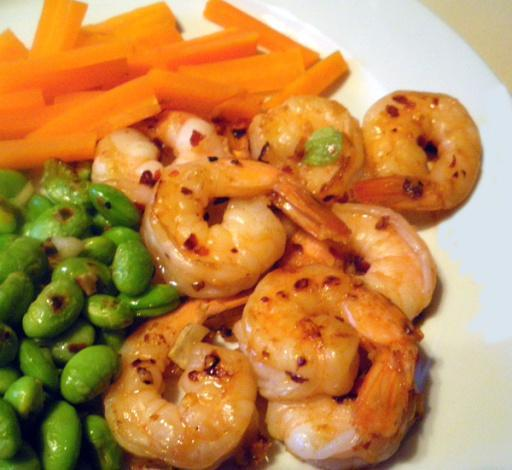
\includegraphics[width=0.24\linewidth]{figures/FoodSeg103_examples/img1.jpg} &
            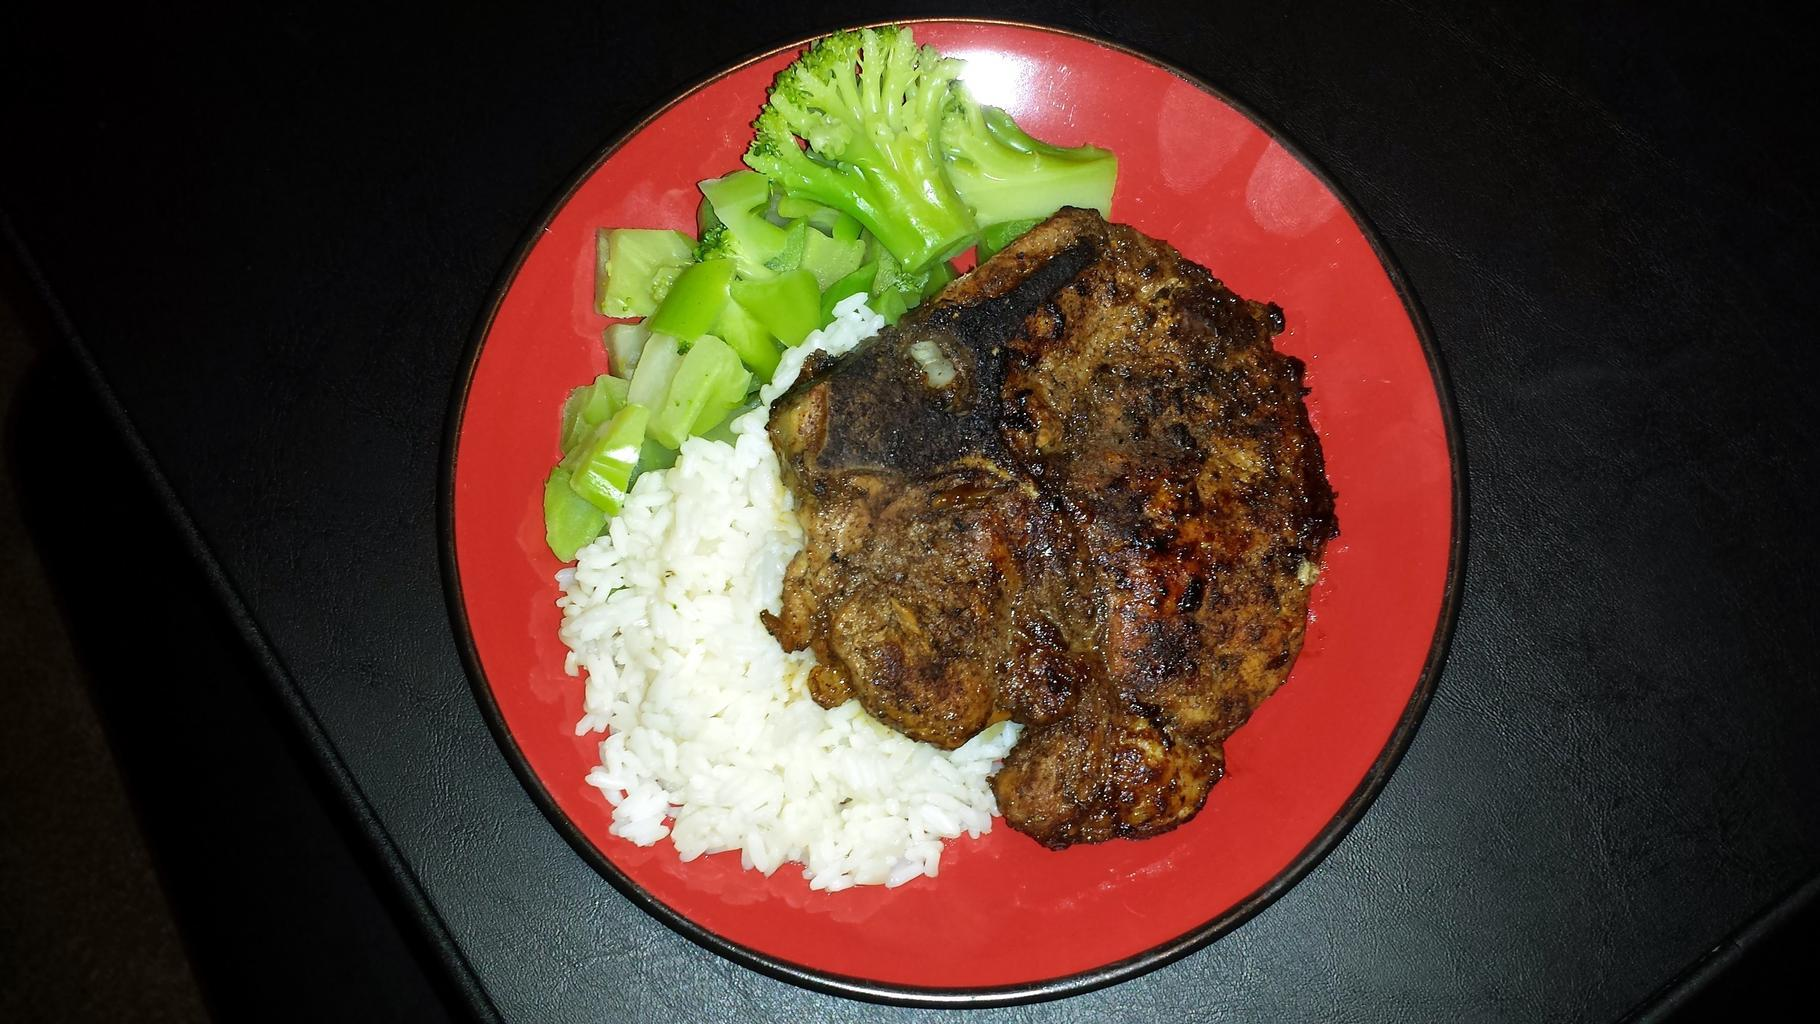
\includegraphics[trim={12.5cm 0cm 12.5cm 0cm},clip, width=0.24\linewidth]{figures/FoodSeg103_examples/img2.jpg} &
            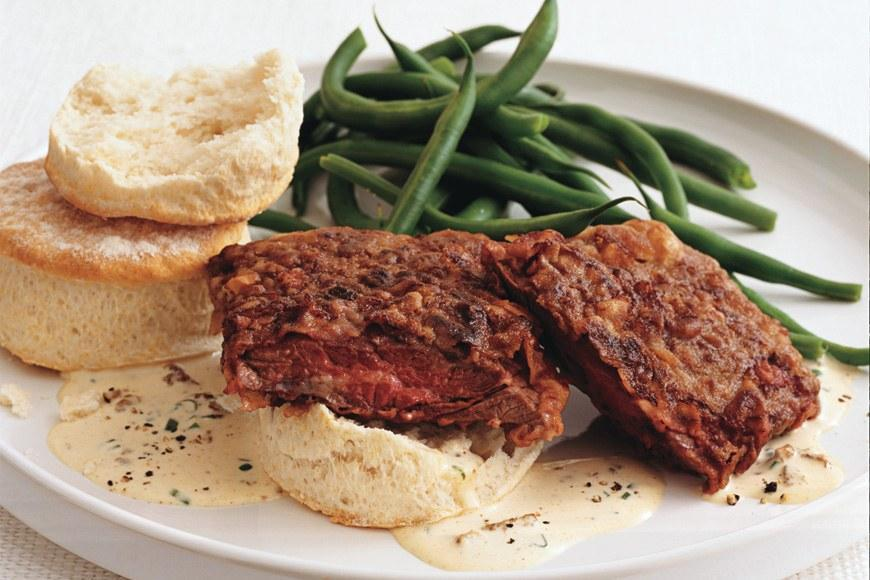
\includegraphics[trim={4.2cm 0cm 4.2cm 0cm},clip, width=0.24\linewidth]{figures/FoodSeg103_examples/img3.jpg} &
            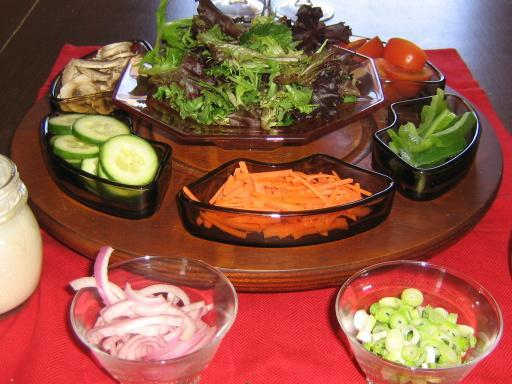
\includegraphics[trim={1.7cm 0cm 1.7cm 0cm},clip, width=0.24\linewidth]{figures/FoodSeg103_examples/img4.jpg} \\
            
\includegraphics[width=0.24\linewidth]{figures/FoodSeg103_examples/img1_mask.jpg} &
            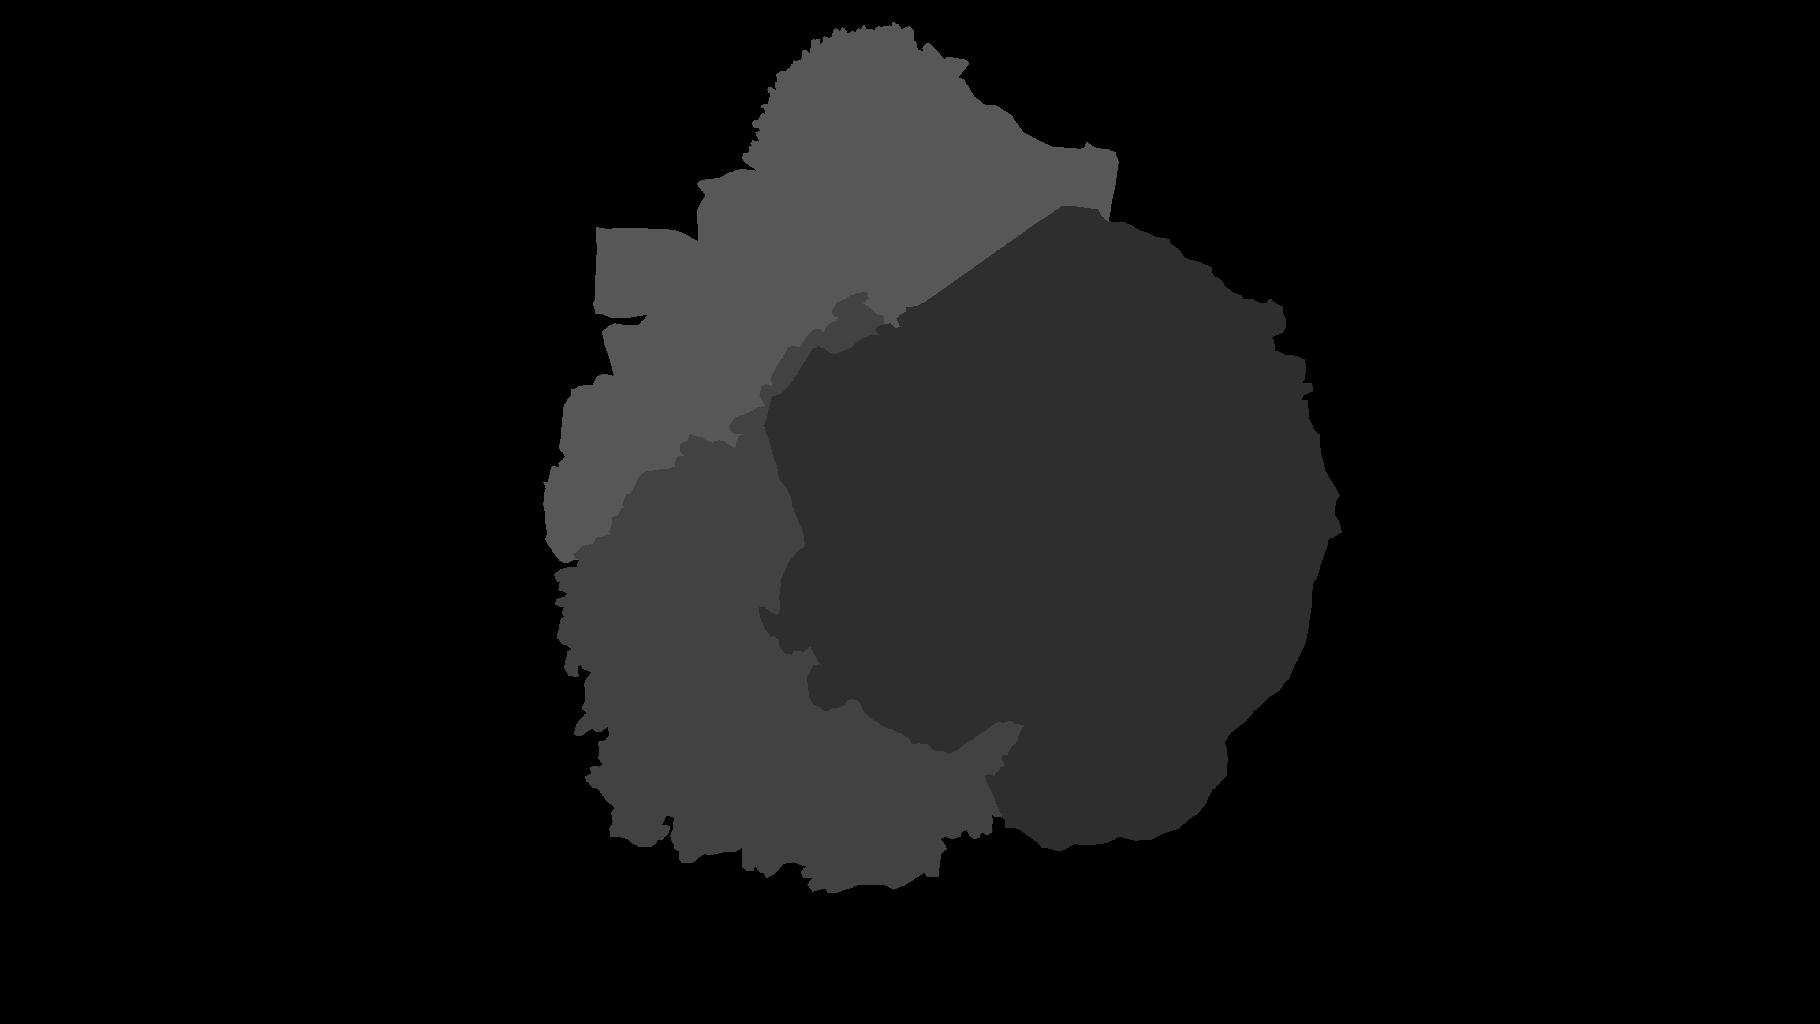
\includegraphics[trim={12.5cm 0cm 12.5cm 0cm},clip, width=0.24\linewidth]{figures/FoodSeg103_examples/img2_mask.jpg} &
            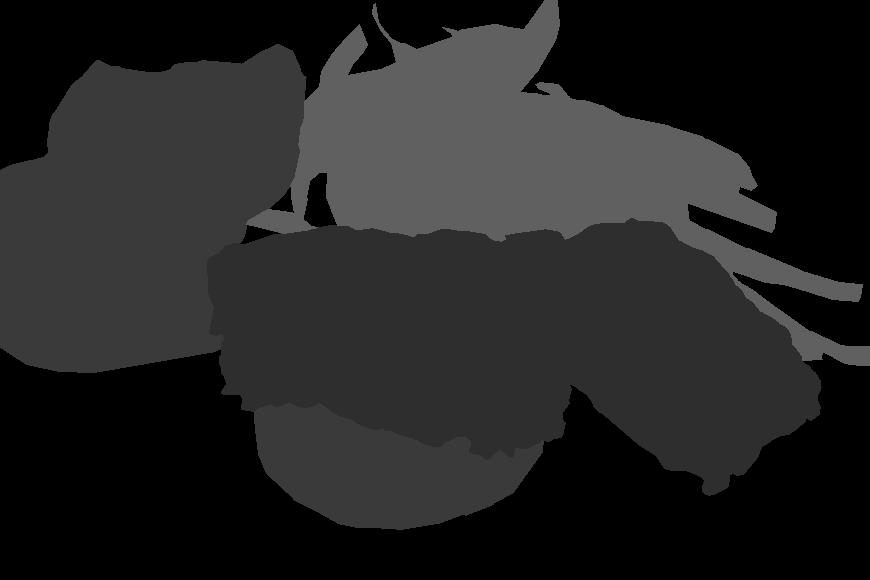
\includegraphics[trim={4.2cm 0cm 4.2cm 0cm},clip, width=0.24\linewidth]{figures/FoodSeg103_examples/img3_mask.jpg} &
            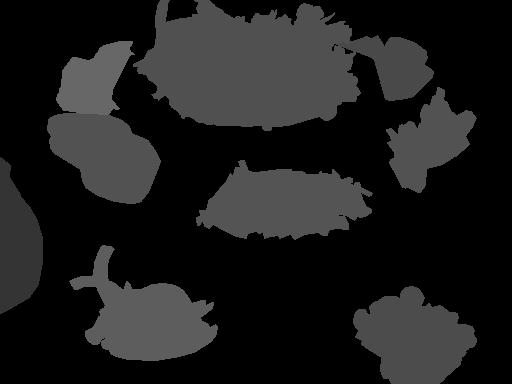
\includegraphics[trim={1.7cm 0cm 1.7cm 0cm},clip, width=0.24\linewidth]{figures/FoodSeg103_examples/img4_mask.jpg} \\
            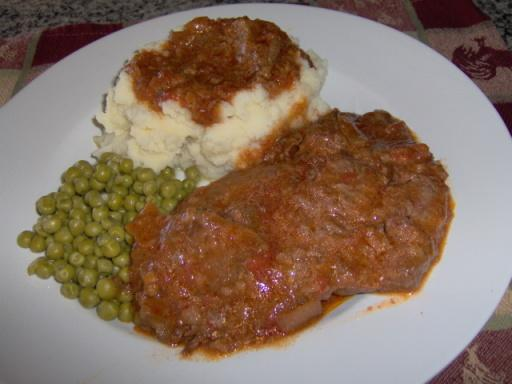
\includegraphics[width=0.24\linewidth]{figures/FoodSeg103_examples/img5.jpg} &
            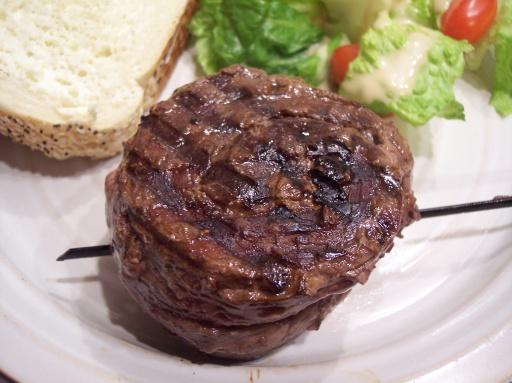
\includegraphics[width=0.24\linewidth]{figures/FoodSeg103_examples/img6.jpg} &
            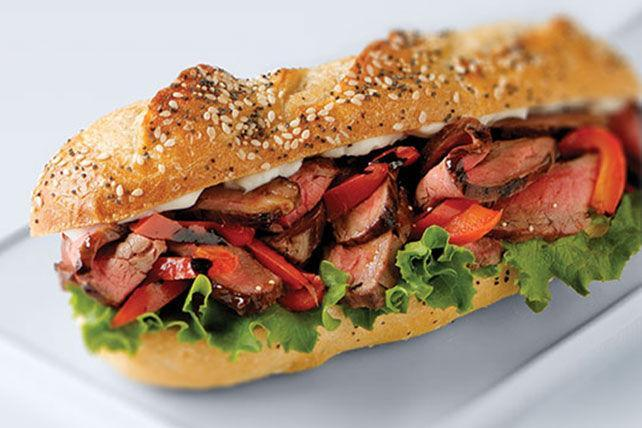
\includegraphics[trim={1.3cm 0cm 1.3cm 0cm},clip, width=0.24\linewidth]{figures/FoodSeg103_examples/img7.jpg} &
            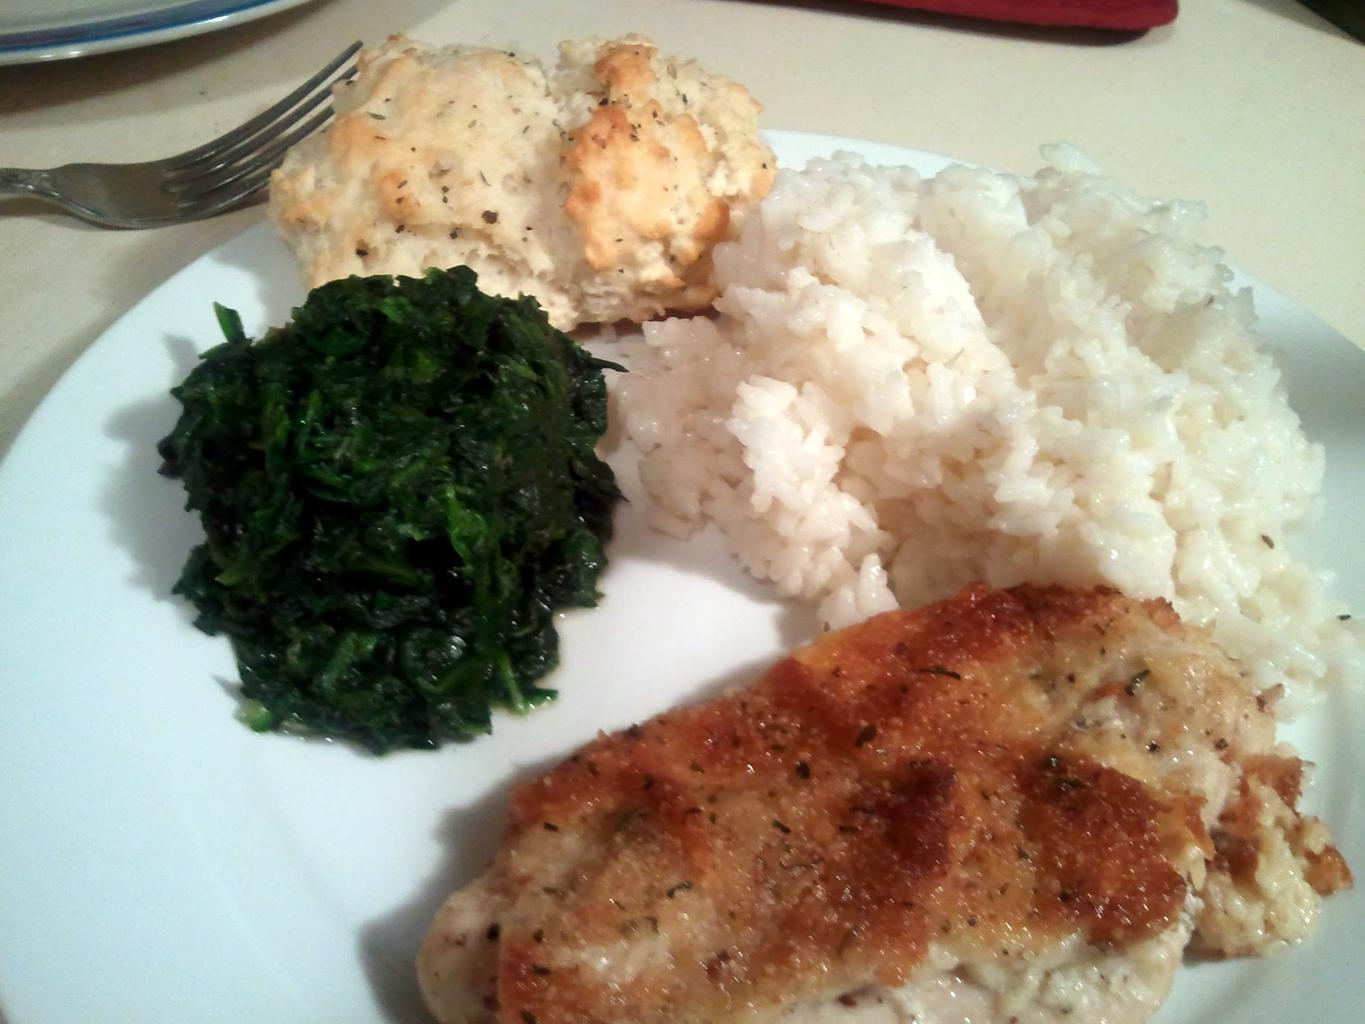
\includegraphics[width=0.24\linewidth]{figures/FoodSeg103_examples/img8.jpg} \\
            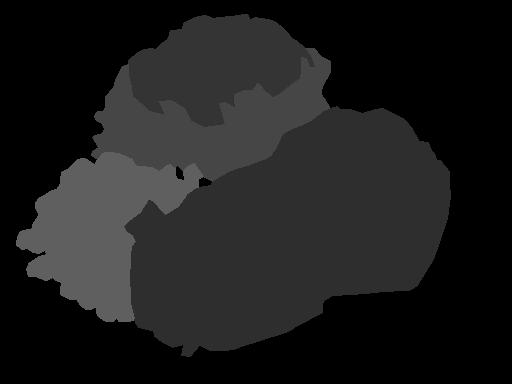
\includegraphics[width=0.24\linewidth]{figures/FoodSeg103_examples/img5_mask.jpg} &
            
\includegraphics[width=0.24\linewidth]{figures/FoodSeg103_examples/img6_mask.jpg} &
            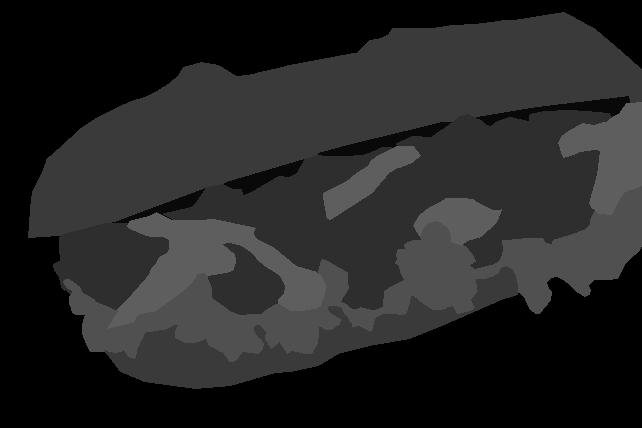
\includegraphics[trim={1.3cm 0cm 1.3cm 0cm},clip, width=0.24\linewidth]{figures/FoodSeg103_examples/img7_mask.jpg} &
            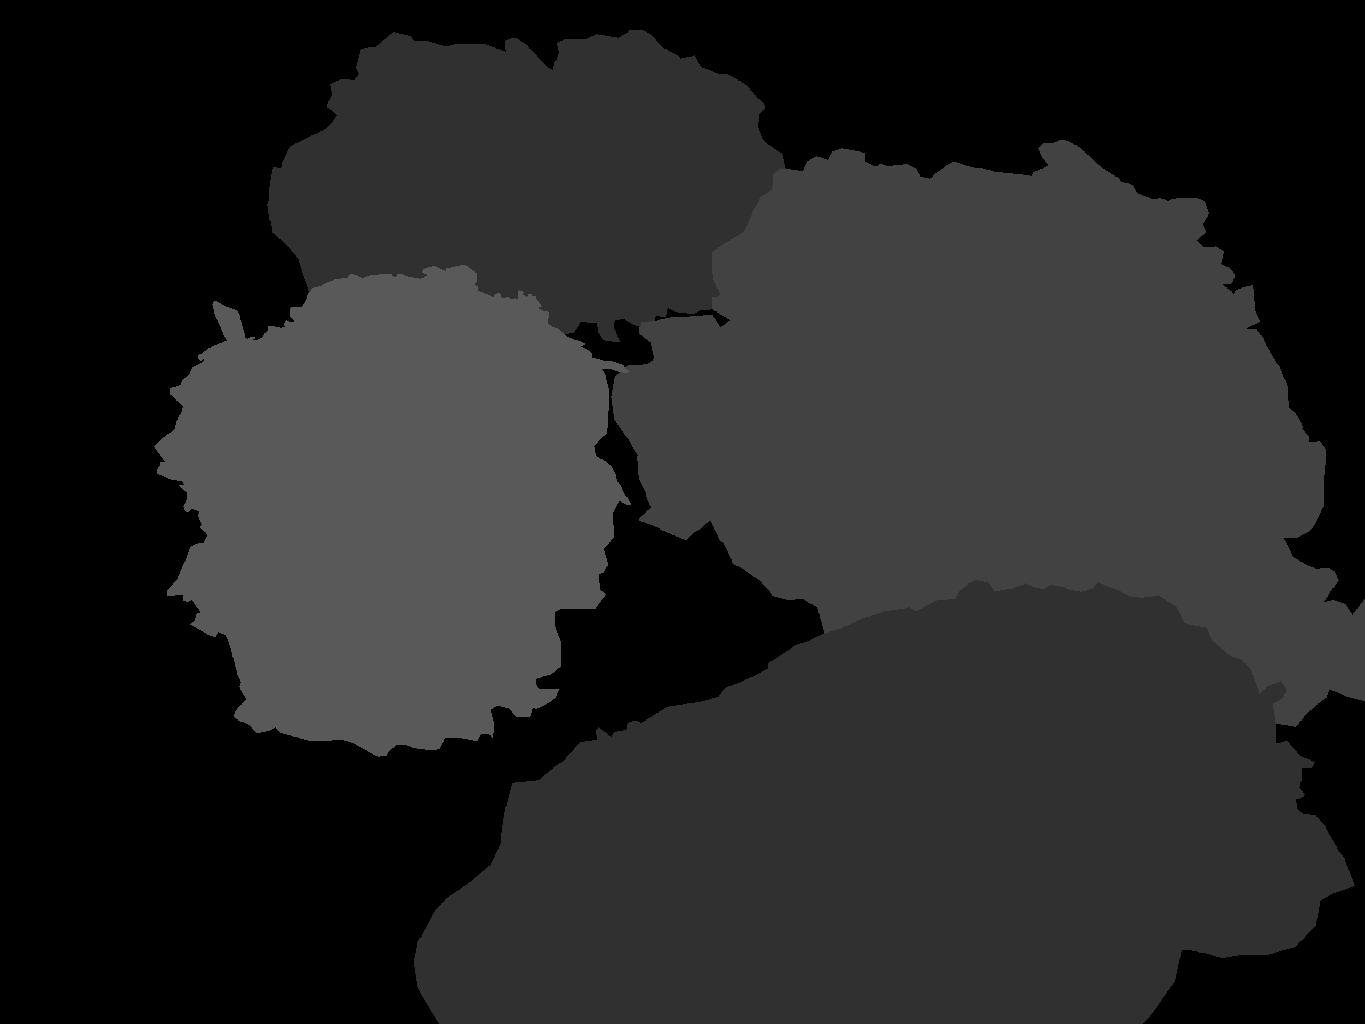
\includegraphics[width=0.24\linewidth]{figures/FoodSeg103_examples/img8_mask.jpg} \\
            \end{tabular}
            % TODO: Ni jasno katera maska pripada kateri sliki
            \caption{Primeri vzorcev in pripadajočih segmentacijskih mask iz podatkovne zbirke FoodSeg103~\cite{src:wu2021large}. Na maskah sivinska vrednost piksla predstavlja indeks razreda, ki mu piksel pripada.}
            \label{fig:foodseg103vzorci}
        \end{figure}

        % Statistične lastnosti, porazdelitev
        Zbirke slik hrane so praviloma močno neuravnotežene. Posamezni razredi sestavin oziroma jedi so bistveno pogostejši od drugih, na porazdelitev pa vplivajo tudi pristranskosti pri sestavljanju podatkovnih zbirk~\cite{src:wu2021large}. Tudi FoodSeg103 izkazuje izrazito nesimetrično porazdelitev v desno (angl. \textit{long-tailed distribution}). Najmanj pogosti razredi se pojavijo le na nekaj deset slikah, najpogostejši pa na več kot 2000 slikah, tj. skoraj tretjini zbirke. Izvorna porazdelitev je prikazana v prilogi~\ref{sct:appendixA}. Na razred je v povprečju na voljo zgolj $252$ slik. Najpogostejši razred (\emph{kruh}) se pojavi v 1402 vzorcih, najredkejši (\emph{alge}, angl. \textit{kelp}) pa v zgolj 74 vzorcih.
        Na posamezni sliki je v povprečju prisotnih $4{,}7$ razredov, porazdelitev števila razredov pa je prikazana na sliki~\ref{fig:foodseg103_orig_num_classes_per_image}.
        
        \begin{figure*}[h]
            \centering
            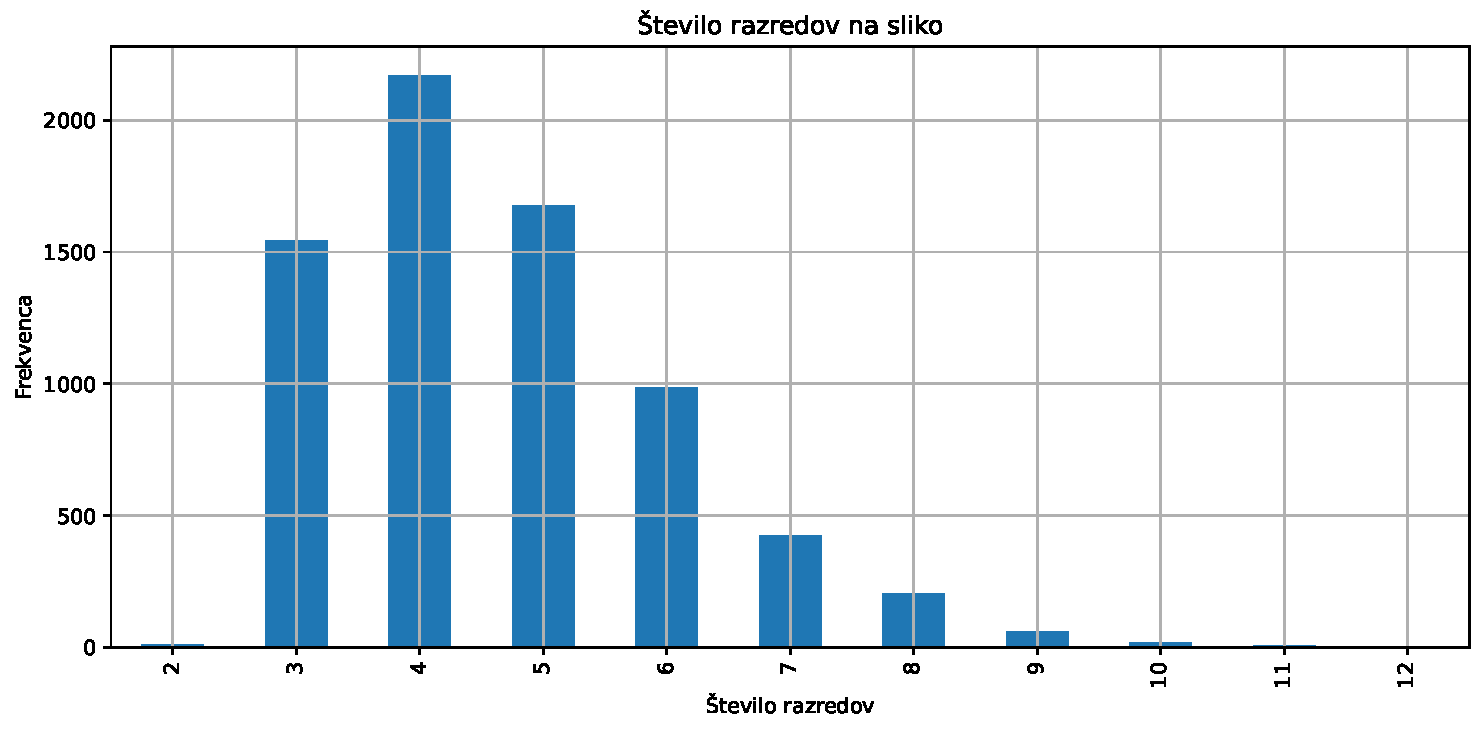
\includegraphics[width=\linewidth]{figures/num_classes_per_image.pdf}
            % TODO: preveri odmik med opisom in sliko
            \caption{Prikaz števila razredov na posamezno sliko v izvorni FoodSeg103 zbirki.}
            \label{fig:foodseg103_orig_num_classes_per_image}
        \end{figure*}
    
        % TODO: Ekstra statistika?

        % Težavnost, izhodiščni rezultati
        Avtorji na FoodSeg103 z modelom DeepLabV3+~\cite{src:chen2017deeplab} dosegajo uspešnost do 34{,}2~\% po metriki mIoU. Na zbirkah UECFoodPix~\cite{src:ege2019new} in UECFoodPix Complete~\cite{src:okamoto2021uec} isti model doseže $41{,}6\,\%$ oziroma $55{,}5\,\%$ po metriki mIoU, na zbirki Cityscapes~\cite{src:cordts2016cityscapes} pa 79{,}0~\% po metriki mIoU.
        Avtorji so na FoodSeg103 učili tudi druge modele, s katerimi so dosegli do 43{,}9~\% po metriki mIoU.
        V kasnejših delih, ki se ukvarjajo s FoodSeg103, poročajo o nekoliko višjih vrednostih, na primer 46{,}4~\%~\cite{src:lan2023foodsam} z modelom FoodSAM in 48{,}7~\%~\cite{src:chen2024ingredsam} z modelom IngredSAM.
        Navedeni rezultati nakazujejo, da je FoodSeg103 zahtevna zbirka.
        K težavnosti prispevata neuravnoteženost razredov in velika znotrajrazredna varianca zaradi različnih načinov priprave hrane. Dodatno so razredi med seboj pogosto vizualno podobni, zato je medrazredna varianca nižja. To je tipična lastnost podatkovnih zbirk hrane in sestavin~\cite{src:wu2021large}.

        % Na kak način smo jo poenostavili
        \subsection{Poenostavitev} \label{sct:eir-podatkovnazbirka-poenostavitev}

            % 1. splošno zmanjšanje kompleksnosti
            Zaradi zahtevnosti zbirke smo želeli kompleksnost zbirke zmanjšati. Poenostavitve je možno uvesti na različne načine. V nadaljevanju naštejemo nekatere izmed pristopov na voljo.
            \begin{itemize}
                \item Na ravni mask lahko dvignemo prag za zelo majhne regije in premajhne segmente ignoriramo. Uvedemo lahko tudi morfološke operacije (odpiranje, zapiranje), ki zgladijo meje in zmanjšajo šum.
                \item Na ravni slik lahko omejimo izbiro na primere z manjšim številom hkrati prisotnih razredov. S tem zmanjšamo prekrivanja in modelu olajšamo nalogo.
                \item Na ravni oznak lahko združimo razdrobljene kategorije v širše nadrazrede na podlagi videza in funkcionalnih lastnosti. Primer bi bili razredi \emph{piščanec}, \emph{svinjina}, \emph{govedina} in \emph{riba}, ki jih lahko združimo v kategorijo \emph{meso}.
                \item Ohranimo le najpogostejše razrede, zelo redke (npr. \emph{alge}, \emph{bambusovi kalčki}) pa odstranimo iz učenja in evalvacije.
            \end{itemize}

            Združevanje v širše kategorije je smiselno, saj pri tem ne zmanjšamo velikosti podatkovne zbirke, vendar je potrebno jasno določiti, katere kategorije so si po lastnostih dovolj podobne, da jih lahko združimo.
            % 2. Zmanjšanje števila razredov
            Zaradi enostavnosti smo raje izbrali zadnjo možnost, torej poenostavitev z ohranitvijo le najpogostejših razredov. Tako skrajšamo rep porazdelitve, zmanjšamo neuravnoteženost in povečamo število učnih primerov za najmanj pogoste izmed ohranjenih razredov. Hkrati zmanjšamo skupno število razredov, kar poenostavi končni model. Kot kriterij smo uporabili prisotnost razredov v podatkovni zbirki (glej prilogo~\ref{sct:appendixA}).

            % 3. Odstranjevanje razredov
            Na večini slik je prisotnih več razredov hkrati, zato obstaja več pristopov za odstranjevanje izbranih razredov. Ena izmed možnost je, da maske neželenih razredov prepišemo v ozadje. Druga možnost je, da odstranimo vse slike, ki vsebujejo katerikoli neželeni razred.
            Izbrali smo slednjega, saj bolje ohrani kakovost podatkovne zbirke. % V kolikor maske neželenih razredov prepišemo v ozadje, ...
            % Smo tu naredili kak eksperiment?

            % 4. Koliko razredov odstranimo
            Kje torej v porazdelitvi izvesti rez? Če ohranimo 30 razredov, kar predstavlja 29~\% vseh razredov, zmanjšamo velikost zbirke za 60{,}4~\%, na skupno $2815$ vzorcev. Povprečno število vzorcev na razred postane $323 \pm 189$. Iz porazdelitve na sliki~\ref{fig:class_freq_30} je razvidno, da je najmanj zastopan razred prisoten na $79$ slikah, najbolj zastopan pa na $705$.

            Če ohranimo zgolj 20 razredov, to je 19~\% vseh razredov, se velikost zbirke zmanjša za 77~\%, na skupno $1634$ vzorcev. Povprečno število vzorcev na razred tako postane $261 \pm 108$. Iz porazdelitve na sliki~\ref{fig:class_freq_20} je razvidno, da je najmanj zastopan razred prisoten na $122$ slikah, najbolj zastopan pa na $481$.

            Večje število ohranjenih razredov pomeni večjo podatkovno zbirko za učenje, hkrati pa tudi zahtevnejšo nalogo za model. Za nadaljnje eksperimente smo zato ohranili 30 najpogostejših razredov in tako oblikovali poenostavljeno različico zbirke FoodSeg103.
            % Tu lahko dodamo graf, ki povezuje število izbranih razredov z velikostjo dataseta, in ponazori zakaj smo se odločili za ravno 30 razredov.
            % Dodatne lastnosti poenostavljene podatkovne zbirke?

            \begin{figure*}[h]
                \centering
                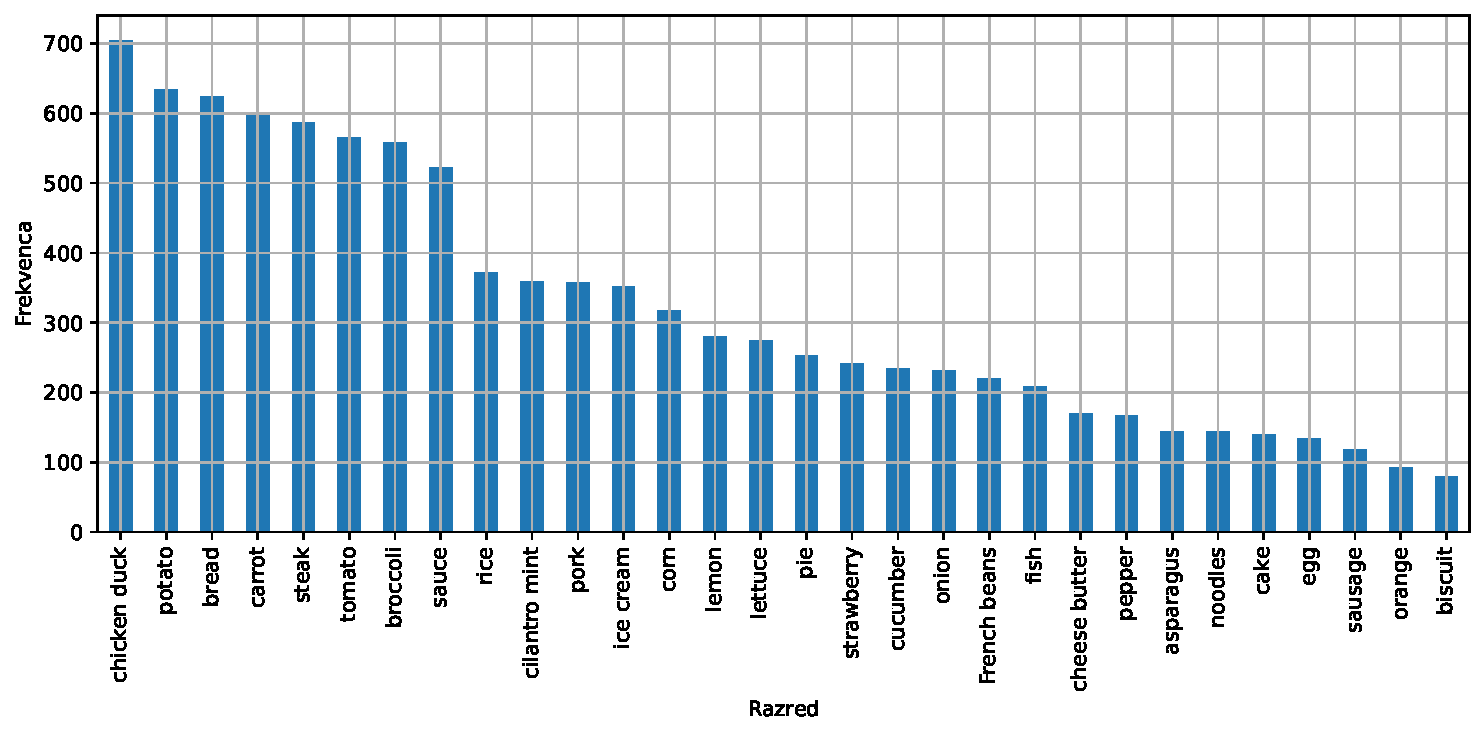
\includegraphics[width=\linewidth]{figures/class_frequency_trimmed_30.pdf}
                % TODO: Prevelik odmik med opisom in sliko
                \caption{Distribucija razredov v zbirki FoodSeg103, poenostavljeni na 30 razredov.}
                \label{fig:class_freq_30}
            \end{figure*}
            
            \begin{figure*}[h]
                \centering
                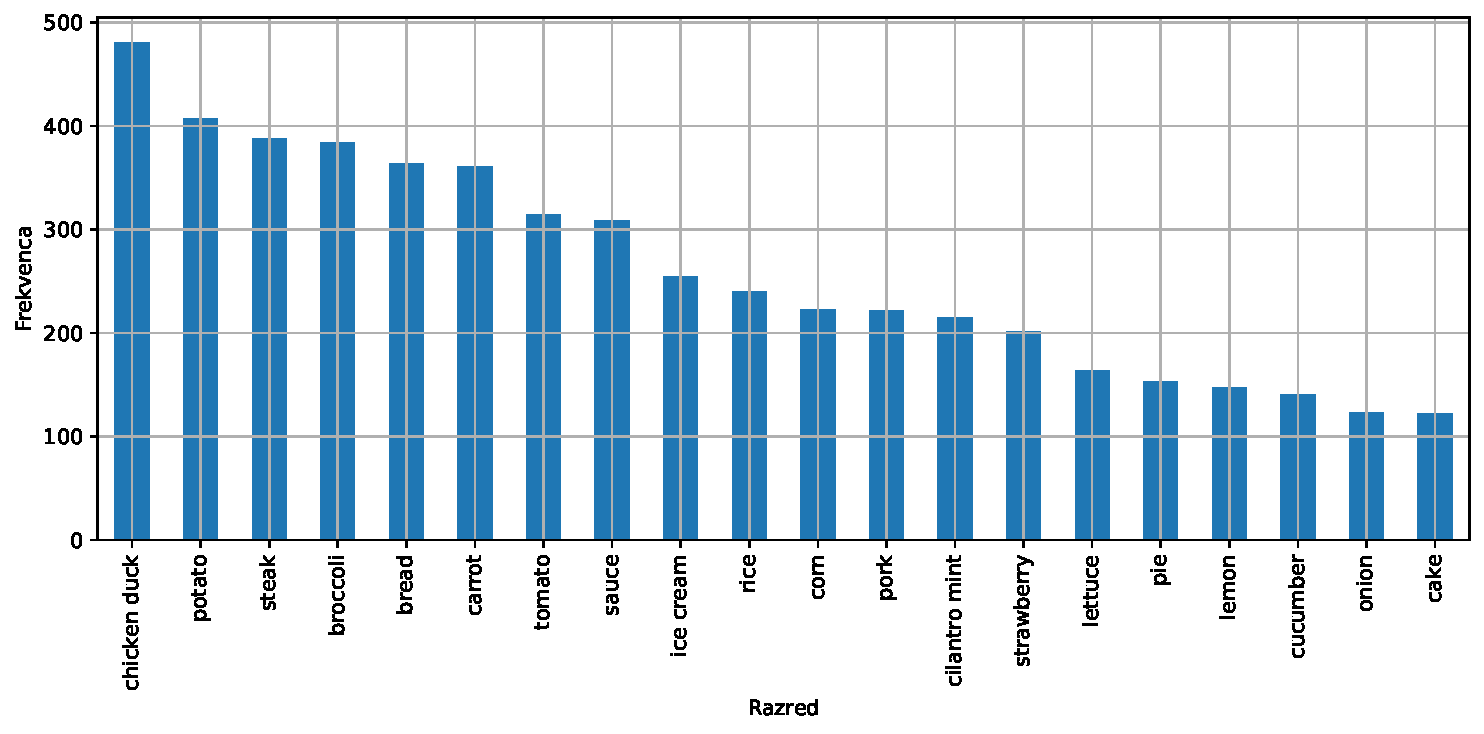
\includegraphics[width=\linewidth]{figures/class_frequency_trimmed_20.pdf}
                % TODO: Prevelik odmik med opisom in sliko
                \caption{Distribucija razredov v zbirki FoodSeg103, poenostavljeni na 20 razredov.}
                \label{fig:class_freq_20}
            \end{figure*}
        
            % TODO: Evalvacija dataseta z neželenimi razredi danimi v ozadje - konkretni rezultati (poberi iz zapiskov eksperimentov)
            % TODO: Evalvacija dataseta z odstranjenimi vzorci - primerjava različnega števila ohranjenih razredov? Sem sploh naredil te eksperimente? Dam to raje pod FOMO eksperimente?

    % Izbrane metrike - performance measures. Mogoče lahko omeniš tut originalne metrike (centroid scoring).
    \section{Izbrane metrike} \label{sct:eir-metrike}

        % TODO: Uvod
        V poglavju \ref{sct:eir-metrike-izvorna} podamo opis metrik, uporabljenih v izvorni implementaciji modela FOMO. Ker v tem delu ne uporabljamo pristopa s središči, smo pristop prilagodili, kot je opisano v poglavju \ref{sct:eir-metrike-prilagojena}.
        % - Izvorne metrike, arugment zakaj jih ne uporabljamo
        % - Prilagojena implementacija metrik
        
        % Opis splošnih metrik, torej P, R, F1, IoU in mIoU. prestavi definicije iz izvorne implementacije.
        Splošne metrike, ki jih uporabljamo v tem delu, so natančnost (angl. \textit{precision}, enačba~\ref{eq:prec}), ki meri delež pravilnih pozitivnih napovedi med vsemi pozitivnimi napovedmi, priklic (angl. \textit{recall}, enačba~\ref{eq:recall}), ki meri delež pravilno zaznanih pozitivnih primerov med vsemi dejanskimi pozitivnimi, in mera F1 (enačba~\ref{eq:f1}), ki je harmonična sredina natančnosti in priklica.
        V kontekstu segmentacije uporabljamo še presek nad unijo (angl. \textit{intersection over union}, IoU, enačba~\ref{eq:iou}) kot standardno segmentacijsko metriko.

        \begin{equation}
            P = \frac{TP}{TP + FP}
            \label{eq:prec}
        \end{equation}
        \begin{equation}
            R = \frac{TP}{TP + FN}
            \label{eq:recall}
        \end{equation}
        \begin{equation}
            F1 = \frac{2 P R}{P + R}
            \label{eq:f1}
        \end{equation}
        \begin{equation}
            \operatorname{IoU}(A,B) = \frac{|A \cap B|}{|A \cup B|}
            \label{eq:iou}
        \end{equation}

        \paragraph{Povprečenje večrazrednih metrik} \label{sct:eir-metrike-povprecenje}
        
            % Uporabili smo makro povprečenje. Uporabili scikit learn implementacijo, ker keras/tf implementacija ni podpirala izbire načina povprečenja. Dodaj definicije za mikro in makro povprečenje, kaj je namen obeh in zakaj smo izbrali makro.
            Pri večrazrednih nalogah je več načinov, kako z eno skalarno mero povzeti uspešnost čez vse razrede. V tej nalogi za natančnost, priklic in mero F1 uporabljamo pristop makro povprečenja. Pri tem metriko najprej izračunamo za vsak razred, nato pa vzamemo neuteženo povprečje po razredih, kot je prikazano v enačbah \ref{eq:prec_macro}, \ref{eq:recall_macro} in \ref{eq:f1_macro}.
            Podobno pri metriki IoU uporabljamo srednjo vrednost preseka nad unijo (angl. mean intersection over union, mIoU). Najprej izračunamo IoU za vsak razred, nato pa vzamemo neuteženo povprečje po razredih.

            % Vse v nadaljevanju navedene metrike so povprečene čez vse razrede, razen če je navedeno drugače.

            \begin{equation}
                P_{\text{makro}} = \frac{1}{N}\sum_{i=1}^N P_{i}
                \label{eq:prec_macro}
            \end{equation}
            \begin{equation}
                R_{\text{makro}} = \frac{1}{N}\sum_{i=1}^N R_{i}
                \label{eq:recall_macro}
            \end{equation}
            \begin{equation}
                F1_{\text{makro}} = \frac{1}{N}\sum_{i=1}^N F1_{i}
                \label{eq:f1_macro}
            \end{equation}

        % Originalne FOMO metrike (centroid scoring)
        \subsection{Izvorna implementacija} \label{sct:eir-metrike-izvorna}

            V nadaljevanju povzamemo, kako so avtorji FOMO izvorno implementirali metrike, v naslednjem poglavju pa opišemo še spremembe, ki smo jih uvedli v kontekstu tega dela.

            % To sem dal na začetek pod splošen opis
            % Med učenjem se na validacijskem naboru poročajo natančnost (angl. \textit{precision}, enačba~\ref{eq:prec}), ki meri delež pravilnih pozitivnih napovedi med vsemi pozitivnimi napovedmi, priklic (angl. \textit{recall}, enačba~\ref{eq:recall}), ki meri delež pravilno zaznanih pozitivnih primerov med vsemi dejanskimi pozitivnimi, in mera F1 (enačba~\ref{eq:f1}), ki je harmonična sredina natančnosti in priklica.
            Kot je opisano v poglavju~\ref{sct:fomo_orig_postprocessing}, je obdelan izhod izvorne implementacije modela nabor središč razpoznanih rojev, vsakemu središču pa je pripisan razpoznan razred.
            Avtorji za izračun metrik podatkovno zbirko obdelajo tako, da vsakemu prisotnemu objektu določijo njegovo referenčno središče. Nato za vsako središče, ki ga je napovedal model, najdejo najbližje referenčno središče in ju primerjajo. V kolikor je razdalja med njima manjša od izbrane mejne vrednosti in se predviden razred roja ujema z referenčnim, se objekt smatra za pravilno razpoznan.

            Iz teh ujemanj za posamezen razred oblikujejo konfuzijsko matriko ter izpeljejo vrednosti TP, FP, TN in FN, na podlagi teh pa izračunajo končne metrike natančnosti, priklica in F1. \mbox{Razred ozadja}, tipično označen z indeksom 0, je izločen iz metrik. Ker v tem delu ne uporabljamo pristopa s središči, smo postopek izračuna metrik prilagodili in vrednosti v konfuzijski matriki izračunali brez uporabe središč rojev.

        \subsection{Prilagojena implementacija} \label{sct:eir-metrike-prilagojena}

            V nadaljnih eksperimentih smo izbrali dva pristopa k implementaciji
            metrik: \textbf{metrike na ravni pikslov} in \textbf{metrike na
            ravni prisotnosti razredov}. Razred ozadja je v vseh primerih
            izključen iz izračunov. V
            poglavju~\ref{sct:fomo_custom_postprocessing}
            smo uvedli praga $\tau$ in $\nu$, slednjega pa lahko v spodaj opisanih pristopih uporabimo za
            uravnavanje razmerja med natančnostjo in priklicem. Višji prag tako
            zmanjšuje število lažnih pozitivnih primerov, nižji prag pa število
            spregledanih pozitivnih primerov.

            \paragraph{Metrike prisotnosti razredov}
            
            % Class presence P, R, F1
            
            %Metrike na ravni pikslov upoštevajo informacijo o lokalizaciji, ki
            %za naš končni problem ni ključna. Zato elemente konfuzijske matrike
            %izračunamo tudi na alternativen način, in sicer na ravni
            %prisotnosti razredov na sliki. Tak pristop obravnava nalogo kot
            %večoznačno klasifikacijo.
            Pri tem pristopu uporabimo modificirano naknadno obdelavo, kot je opisana v \ref{sct:metodologija-fomo-processing}. Model tako izvaja večoznačno razvrščanje (angl. multi-label classification) in ne ohranja informacije o lokaciji.
            % Kaj točno se dogaja
            %Podobno kot pri pristopu na ravni pikslov najprej za vsak izhodni piksel določimo razred na podlagi verjetnostne porazdelitve in praga \(\tau\).
            %V naknadni obdelavi smo uvedli prag $\tau$ in Uvedemo še prag \(\nu \in \mathbb{N}_0\), ki določa minimalno število pikslov, da razred štejemo kot prisoten. Za vsak razred preštejemo število napovedanih pikslov in če je to število vsaj \(\nu\), razred označimo kot prisoten.
            Končni izhod je binarni vektor prisotnosti razredov na sliki, pri čemer razred ozadja izključimo pri izračunu metrik.
            % Zakaj ne merimo metrik za razred ozadja? Zato ker nas ne zanima kako dobro model zna razpoznat ozadje.

            Nato za vsak razred sestavimo konfuzijsko matriko velikosti
            \(2\times 2\) (skupaj \(n\) takih matrik). Iz njih izračunamo
            natančnost $P_r$, priklic $R_r$ in mero $F1_r$ po
            definicijah~\ref{eq:prec},~\ref{eq:recall}
            in~\ref{eq:f1}.
            Tak pristop meri uspešnost v obliki, ki jo zahteva naš problem, torej prisotnost sestavine na sliki brez upoštevanja lokacije.
            % TODO: To bi verjetn moglo it v diskusijo...
            % Ker je rezultat razdeljen na več konfuzijskih matrik, je manj neposredno viden vzorec zamenjav med razredi.
            
            % TODO: Slika ki ponazarja class presence postopek


            \paragraph{Metrike na ravni pikslov.} \label{sct:eir-metrike-pixel}

            Ta pristop izračuna elemente konfuzijske matrike na ravni
            slikovnih elementov.
            % Navezi se na naknadno obdelavo
            %Za vsak slikovni element v napovedani maski vzamemo predikcije verjetnosti razredov in določimo razred z največjo verjetnostjo. Če noben razred ne preseže praga $\tau$, pikslu pripišemo ozadje.
            Uporabimo nizkoločjivostno segmentacijsko masko, ki je rezultat 2. koraka v modificirani naknadni obdelavi, opisani v \ref{sct:fomo_custom_postprocessing}.
            S primerjanjem istoležnih celic med predikcijo in referenčno masko dobimo za vsak razred število pravilnih pozitivnih, napačnih pozitivnih, spregledanih pozitivnih in pravilnih negativnih predikcij.
            Iz teh vrednosti sestavimo konfuzijsko matriko velikosti \(n\times n\), kjer \(n\) označuje število obravnavanih razredov brez ozadja. Na podlagi te matrike nato izračunamo natančnost $P_p$, priklic $R_p$ in mero $F1_p$.

            % Motivacija, zakaj bi to hotel
            Ta pristop zaradi primerjave istoležnih pikslov mask evalvira tudi
            lokalizacijsko sposobnost modela. Čeprav je ta informacija za naš
            končni problem nepomembna, nam nastala konfuzijska matrika omogoča
            dober vpogled v lastnosti modela in izpostavi tipične napake ter
            šibkejše razrede.

            % TODO: Slika, ki ponazarja per-pixel postopek. Lahko screenshot iz
            % tensorboarda, urejen v inkscapu. Omeni tudi, da je ground truth
            % downscalan na isto nizko resolucijo, mogoče celo povej katero
            % interpolacijo si uporabil. Caption: Tako dobljeno gosto kodiranje
            % primerjamo z referenčno masko na isti ločljivosti. Ker FOMO vrača
            % nizkoločljivostne izhode, tipično \(8\times 8\) ali \(16\times
            % 16\), pred začetkom umerimo tudi referenčne maske na isto mrežo.

            % TODO: Mogoče polinkaj na primer kakšne konfuzijske matrike, če ga imaš.

            % To sem dal malo višje, pod splošen opis
            %Ker v tem pristopu izhod modela obravnavamo kot segmentacijsko
            %masko, v nekaterih primerih poročamo še \textbf{presek nad unijo}
            %(angl. \textit{intersection over union}, IoU, enačba~\ref{eq:iou})
            %kot standardno segmentacijsko metriko.
            Poleg izračuna metrik $P_p$, $R_p$ in $F1_p$ lahko s primerjanjem
            predikcijske in referenčne maske izračunamo metriko IoU.
            Uporaba te metrike nam omogoči neposredno primerjavo z rezultati,
            ki so jih druge študije dosegle na isti podatkovni zbirki, vendar
            je uporaba pri grobi segmentacijski maski problematična za manjše
            objekte. FOMO vrača nizkoločljivostne izhode, tipično \(8\times 8\)
            ali \(16\times 16\), kar pomeni, da pred začetkom tudi referenčne
            maske pretvorimo na isto ločljivost, posamezen piksel pa
            predstavlja odsek vhodne slike. V kolikor objekt v referenci
            zavzame en sam piksel, lahko IoU za ta razred zavzame zgolj $0{,}0$
            ali $1{,}0$, kar je izrazito nezvezno.

    \section{Eksperimenti} \label{sct:eir-eksperimenti}
    
        % TODO: kratek opis kaj imamo v tem poglavju
        
        \subsection{Model FOMO} \label{sct:eksperimenti-fomo}
            
            % TODO: kratek opis kaj imamo v tem poglavju
        
            \paragraph{Validacija okolja z namernim prenaučenjem} \label{sct:eir-eksperimenti-validacija}
                % Single batch overfit eksperiment
                
                Kot začetni preizkus korektnosti učnega okolja izvedemo namerno prenaučenje na zelo majhnem naboru podatkov~\cite{src:karpathy2019recipe}. Mreža se uči in evalvira na zelo majhnem naboru vzorcev, iste podatke uporabimo v vseh epohah. Pričakovani izid je, da se učna izguba približa ničli, napovedi pa se poravnajo z oznakami. Evalvacija in testiranje v tem preizkusu potekata nad istimi vzorci kot učenje, saj preverjamo delovanje podatkovnega cevovoda in učnega okolja. Tak pregled hitro razkrije skrite napake in potrdi, da model in učno okolje lahko sploh učinkovito učita.

                Med tem eksperimentom začasno onemogočimo močne augmentacije ter regularizacijo, nato pa učimo na zelo omejenem naboru podatkov, dokler vrednost kriterijske funkcije ne pade na 0. Če do minimizacije izgube ne pride, to pogosto nakazuje na napako v pripravi podatkov, definiciji izgube ali posodabljanju uteži, zato napako odpravimo pred nadaljnjimi eksperimenti.

                Rezultati na~\ref{fig:overfit_one_batch_plots} in~\ref{fig:overfit_one_batch_example} nakazujejo, da učno okolje uspešno reši majhen nabor podatkov.

                \begin{figure}[t]
                  \centering
                  \setlength{\tabcolsep}{2pt} % space between columns
                  \renewcommand{\arraystretch}{1} % no extra row padding
                  \begin{tabular}{@{}cc@{}}
                  
                        \begin{tikzpicture}
                            \begin{axis}[
                              width=0.5\linewidth,
                              height=0.5\linewidth,
                              xlabel=Epohe,
                              ylabel=Krit. funkcija,
                              grid=both,
                              ymin=0,
                              %legend pos=north east,
                              %legend style={draw=none, fill=none, font=\small}
                              legend style={font=\small}
                            ]
                                \addplot+[thick, mark=none] table [x=Step, y=Value, col sep=comma] {figures/single_batch_test/loss_train_alpha_1.0.csv};
                                \addplot+[thick, mark=none] table [x=Step, y=Value, col sep=comma] {figures/single_batch_test/loss_val_alpha_1.0.csv};
                            \end{axis}
                        \end{tikzpicture}
                  
                        \begin{tikzpicture}
                            \begin{axis}[
                              width=0.5\linewidth,
                              height=0.5\linewidth,
                              xlabel=Epohe,
                              ylabel=F1,
                              grid=both,
                              ymin=0,
                              legend pos=south east,
                              %legend style={draw=none, fill=none, font=\small}
                              legend style={font=\small}
                            ]
                                \addplot+[thick, mark=none] table [x=Step, y=Value, col sep=comma] {figures/single_batch_test/f1_train_alpha_1.0.csv};
                                \addlegendentry{Učna};
                                \addplot+[thick, mark=none] table [x=Step, y=Value, col sep=comma] {figures/single_batch_test/f1_val_alpha_1.0.csv};
                                \addlegendentry{Validacijska};
                            \end{axis}
                        \end{tikzpicture}
                        
                  \end{tabular}
                  % TODO: vsak graf na sliki mora biti enoznačno označen kot npr. (a) (b). Oznake moraš potem uporabiti v opisu slike.
                  \caption{Potek kriterijske funkcije in metrike $F1_r$ skozi namerno prenaučenje z namenom validacije učnega okolja.}
                  \label{fig:overfit_one_batch_plots}
                \end{figure}

                \begin{figure}[h]
                    \centering
                    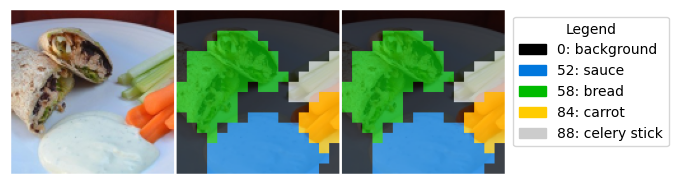
\includegraphics[width=\linewidth]{figures/single_batch_test/overfit_one_batch_example.png}
                    % TODO: preveri odmik med opisom in sliko
                    % TODO: vsak graf na sliki mora biti enoznačno označen kot npr. (a) (b). Oznake moraš potem uporabiti v opisu slike.
                    \caption{Primer inference na modelu, namenjenemu validaciji okolja z namernim prenaučenjem. Od leve proti desni: vhodna slika, izhod modela in referenčna maska.}
                    \label{fig:overfit_one_batch_example}
                \end{figure}
            
            \paragraph{Določanje optimalnih vrednosti za stopnjo učenja} \label{sct:eir-eksperimenti-dolocanje-learning-rate}

                Za določanje stopnje učenja (\textit{learning rate}) uporabimo pristop iz~\cite{src:smith2017cyclical}. V kratkem preizkusu stopnjo učenja enakomerno povečujemo po korakih, od zelo nizke do visoke vrednosti, ter sproti beležimo vrednost kriterijske funkcije. Na dobljenem grafu poiščemo območje največjega izboljševanja, torej točko z najstrmejšim upadom izgube. To točko uporabimo kot začetno stopnjo učenja. V nadaljevanju uporabljamo običajen razpored zniževanja stopnje učenja (npr. zniževanje ob platoju \footnote{Primer takšnega orodja: \url{https://keras.io/api/callbacks/reduce_lr_on_plateau/}}), ki stopnjo postopoma zmanjšuje proti območju, kjer se izboljševanje upočasni. 

                Tak preizkus bistveno zmanjša ugibanje pri izbiri hiperparametra in pogosto skrajša čas učenja. Priporočljivo ga je ponoviti ob vsaki spremembi podatkovne zbirke, arhitekture, velikosti paketa ali kriterijske funkcije. Alternativno lahko dobljeni spodnjo in zgornjo mejo uporabimo tudi pri cikličnem razporedu stopenj učenja~\cite{src:smith2017cyclical}.

                Na sliki~\ref{fig:lr_finder_plots} sta prikazana takšna eksperimenta, prvi za $\alpha=0.35$, drugi pa za $\alpha=1.0$. Oba modela uporabljata izhodno plast za 30 razredov sestavin. Vidimo, da je  najbolj ustrezna začetna stopnja učenja $\eta_0$ v razponu okrog $[5\cdot10^{-4},\,\ 10^{-2}]$, za končno pa je ustrezna okrog $\eta_k = 10^{-5}$. Razvidno je še, da parameter $\alpha$ v razponu $[0.35, 1.0]$ ne vpliva bistveno na primerno vrednost $\eta$.

                \begin{figure}[t]
                  \centering
                  \setlength{\tabcolsep}{2pt} % space between columns
                  \renewcommand{\arraystretch}{1} % no extra row padding
                  \begin{tabular}{@{}cc@{}}
                  
                        \begin{tikzpicture}
                            \begin{axis}[
                              width=0.9\linewidth,
                              height=0.7\linewidth,
                              xlabel=$\eta$,
                              ylabel=Krit. funkcija,
                              grid=both,
                              xmode=log,
                              legend pos=north east,
                              %legend style={draw=none, fill=none, font=\small}
                              legend style={font=\small}
                            ]
                                \addplot+[thick, mark=none] table [x=lrs, y=losses, col sep=comma] {figures/lr_finder/alpha_0.35.csv};
                                \addlegendentry{$\alpha=0.35$}
                                \addplot+[thick, mark=none] table [x=lrs, y=losses, col sep=comma] {figures/lr_finder/alpha_1.0.csv};
                                \addlegendentry{$\alpha=1.0$}
                            \end{axis}
                        \end{tikzpicture}
                        
                  \end{tabular}
                  \caption{Potek kriterijske funkcije skozi spreminjajoč se faktor učenja $\eta$. Iz slike je razvidno, da se model najbolje uči pri faktorju $\eta_0$ okrog $10^{-3}$.}
                  \label{fig:lr_finder_plots}
                \end{figure}
                
            
            \paragraph{Učenje na izvirni FoodSeg103 zbirki} \label{sct:eir-ucenje-na-izvirnem-datasetu}

                V tem eksperimentu ocenimo delovanje modela na izvorni, nepoenostavljeni podatkovni zbirki. Preizkusimo dva načina uteževanja. Prvi je enakomerno uteževanje razredov s faktorjem \(100\), kot ga predlagajo avtorji~\cite{src:fomodocs}, pri čemer je ozadje uteženo s faktorjem \(1\). Drugi pristop temelji na frekvenci razredov v zbirki: za vsak razred določimo relativno frekvenco \(f_i\) in vzamemo njen inverz kot utež, tj.\ \(w_i=\tfrac{1}{f_i}\). Na primer, če je \(f_i=0{,}227\), potem je \(w_i=\tfrac{1}{0{,}227}=4{,}405\). Ker je ozadje prisotno na vseh vzorcih, je njegova utež \(w_{\mathrm{bg}}=1{,}0\).

                Za večjo kapaciteto modela nastavimo parameter \(\alpha\) na \(1{,}0\). Prag \(\tau\) nastavimo na \(0{,}2\), prag \(\nu\) pa na \(3\). Vhodno ločljivost nastavimo na \(128 \times 128\) pikslov, izhodno masko pa pomanjšamo za faktor $16$, kar pomeni ločljivost \(8 \times 8\) pikslov. V predprocesiranju uporabimo knjižnico Albumentations\footnote{\url{https://explore.albumentations.ai/}} za augmentacije naključnega obrezovanja (\emph{random resized crop}), naključno vodoravno in navpično zrcaljenje, naključno rotacijo do \(15^{\circ}\) ter naključno spremembo svetlosti in kontrasta. Model učimo v celoti po vseh plasteh (angl. \emph{end-to-end}).

                % Grafi kriterijske funkcije
                \begin{figure}[t]
                  \centering
                  \setlength{\tabcolsep}{2pt} % space between columns
                  \renewcommand{\arraystretch}{1} % no extra row padding
                  \begin{tabular}{@{}cc@{}}
                  
                        \begin{tikzpicture}
                            \begin{axis}[
                              width=0.5\linewidth,
                              height=0.5\linewidth,
                              xlabel=Epohe,
                              ylabel=Krit. funkcija,
                              grid=both,
                              ymin=0,
                              %legend pos=north east,
                              %legend style={draw=none, fill=none, font=\small}
                              legend style={font=\small}
                            ]
                                \addplot+[thick, mark=none] table [x=Step, y=Value, col sep=comma] {figures/full_foodseg103_dataset/uniform_weights/loss_train.csv};
                                \addplot+[thick, mark=none] table [x=Step, y=Value, col sep=comma] {figures/full_foodseg103_dataset/uniform_weights/loss_val.csv};
                            \end{axis}
                        \end{tikzpicture}
                  
                        \begin{tikzpicture}
                            \begin{axis}[
                              width=0.5\linewidth,
                              height=0.5\linewidth,
                              xlabel=Epohe,
                              % ylabel=Krit. funkcija,
                              grid=both,
                              ymin=0,
                              legend pos=south east,
                              %legend style={draw=none, fill=none, font=\small}
                              legend style={font=\small}
                            ]
                                \addplot+[thick, mark=none] table [x=Step, y=Value, col sep=comma] {figures/full_foodseg103_dataset/weights_from_stats/loss_train.csv};
                                \addlegendentry{Učna};
                                \addplot+[thick, mark=none] table [x=Step, y=Value, col sep=comma] {figures/full_foodseg103_dataset/weights_from_stats/loss_val.csv};
                                \addlegendentry{Validacijska};
                            \end{axis}
                        \end{tikzpicture}
                        
                  \end{tabular}
                  \caption{Spreminjanje kriterijske funkcije tekom učenja na izvirni, nepoenostavljeni zbirki FoodSeg103. Levo je izvedba z uniformno uteženimi razredi, desno pa z utežmi na podlagi frekvence razredov.}
                  \label{fig:experiment_full_foodseg103_dataset_loss}
                \end{figure}

                % Kvalitativno
                \begin{figure*}[h!]
                    \centering
                    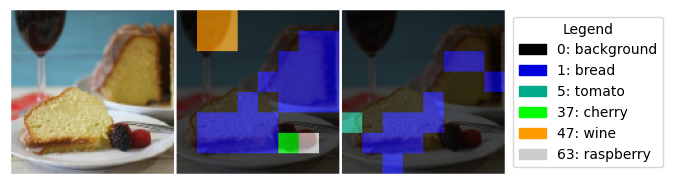
\includegraphics[width=0.8\linewidth]{figures/full_foodseg103_dataset/uniform_weights/example1.png}
                    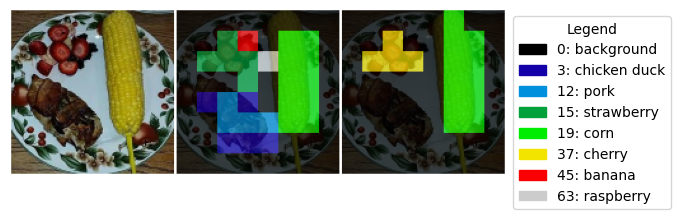
\includegraphics[width=0.8\linewidth]{figures/full_foodseg103_dataset/uniform_weights/example2.png}
                    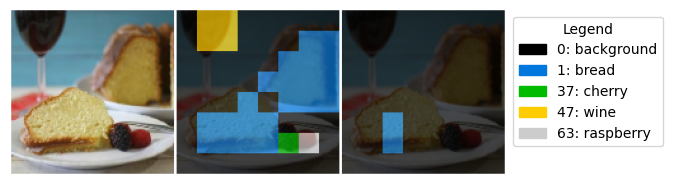
\includegraphics[width=0.8\linewidth]{figures/full_foodseg103_dataset/weights_from_stats/example1.png}
                    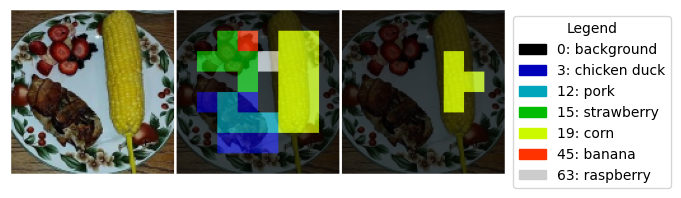
\includegraphics[width=0.8\linewidth]{figures/full_foodseg103_dataset/weights_from_stats/example2.png}
                    % TODO: Manjkajo reference posamezne grafike, uporabi a b c d
                    \caption{Kvalitativni rezultati na izvirni, nepoenostavljeni zbirki FoodSeg103. Od leve proti desni: vhodna slika, referenčna maska, predikcija modela. Zgornji dve sliki sta rezultat izvedbe z uniformnimi utežmi, spodnji dve pa rezultat izvedbe na podlagi frekvence razredov.}
                    \label{fig:experiment_full_foodseg103_dataset_qualitative}
                \end{figure*}
                
                % Tabela rezultatov (f1 class presence, f1 per pixel, iou)
                \begin{table}[t]
                    \centering
                    \begin{tabular}{lccc}
                        \toprule
                        \textbf{Izvedba uteži $w$} & \textbf{F1$_r$} & \textbf{F1$_p$} & \textbf{IoU} \\
                        \midrule
                        Uniformno          & 13{,}8 & 9{,}8 & 6{,}0 \\
                        Frekvenca razredov & 11{,}4 & 7{,}6 & 4{,}3 \\
                        \bottomrule
                    \end{tabular}
                    \caption{Rezultati učenja na polni FoodSeg103 zbirki.}
                    \label{tab:experiment_full_foodseg103_dataset_table}
                \end{table}
                % TODO: Tabela je takoj za sliko

                Namen eksperimenta je določiti izhodiščne vrednosti mer F1 in IoU na izvorni podatkovni zbirki ter oceniti vpliv različnih pristopov uteževanja pri izrazito neuravnoteženi porazdelitvi razredov. Rezultati so prikazani na sliki~\ref{fig:experiment_full_foodseg103_dataset_loss} in v tabeli~\ref{tab:experiment_full_foodseg103_dataset_table}.
                Obe izvedbi izkazujeta slabe rezultate. Pri izvedbi z uteževanjem glede na frekvenco razredov se prenaučenje pojavi bistveno prej, hkrati pa so rezultati na testni množici slabši.
                Kvalitativne vizualizacije na sliki~\ref{fig:experiment_full_foodseg103_dataset_qualitative} so skladne s številčnimi izidi. Izvedba z uteževanjem po frekvenci v večini primerov napove zgolj ozadje, medtem ko enakomerno utežena izvedba da vsaj nekaj napovedi, čeprav so te večinoma nepravilne.

                
            \paragraph{Učenje na poenostavljeni zbirki in primerjava pristopov uteževanja} \label{sct:eir-fomo-simplified-experiments}

                V nadaljnjih eksperimentih uporabimo poenostavljeno podatkovno zbirko in znova preizkusimo dva načina uteževanja razredov. Konfiguracija parametrov ostane podobna kot v odseku~\ref{sct:ucenje-na-izvirnem-datasetu}: \(\alpha=1{,}0\), \(\tau=0{,}2\) in \(\nu=3\). Vhodna ločljivost je \(128 \times 128\) pikslov, izhodna maska pa ima ločljivost \(8 \times 8\) pikslov. V predprocesiranju uporabimo isti nabor augmentacij kot v navedenem odseku.

                % Namen eksperimenta + opis rezultatov objektivno
                Rezultati so prikazani na sliki~\ref{fig:experiment_simplified_foodseg103_dataset_loss} in v tabeli~\ref{tab:experiment_simplified_foodseg103_dataset_table}. V primerjavi z rezultati v poglavju~\ref{sct:ucenje-na-izvirnem-datasetu} doseže ta eksperiment izrazito boljše rezultate, različna uteževanja pa na pridobljene rezultate nimajo izrazitega vpliva.

                % Grafi kriterijske funkcije
                \begin{figure*}[t]
                  \centering
                  \setlength{\tabcolsep}{2pt} % space between columns
                  \renewcommand{\arraystretch}{1} % no extra row padding
                  \begin{tabular}{@{}cc@{}}
                  
                        \begin{tikzpicture}
                            \begin{axis}[
                              width=0.5\linewidth,
                              height=0.5\linewidth,
                              xlabel=Epohe,
                              ylabel=Krit. funkcija,
                              grid=both,
                              ymin=0,
                              %legend pos=north east,
                              %legend style={draw=none, fill=none, font=\small}
                              legend style={font=\small}
                            ]
                                \addplot+[thick, mark=none] table [x=Step, y=Value, col sep=comma] {figures/simplified_foodseg103_dataset/uniform_weights/loss_train.csv};
                                %\addlegendentry{Učna};
                                \addplot+[thick, mark=none] table [x=Step, y=Value, col sep=comma] {figures/simplified_foodseg103_dataset/uniform_weights/loss_val.csv};
                                %\addlegendentry{Validacijska};
                            \end{axis}
                        \end{tikzpicture}
                  
                        \begin{tikzpicture}
                            \begin{axis}[
                              width=0.5\linewidth,
                              height=0.5\linewidth,
                              xlabel=Epohe,
                              % ylabel=Krit. funkcija,
                              grid=both,
                              ymin=0,
                              legend pos=north east,
                              %legend style={draw=none, fill=none, font=\small}
                              legend style={font=\small}
                            ]
                                \addplot+[thick, mark=none] table [x=Step, y=Value, col sep=comma] {figures/simplified_foodseg103_dataset/weights_from_stats/loss_train.csv};
                                \addlegendentry{Učna};
                                \addplot+[thick, mark=none] table [x=Step, y=Value, col sep=comma] {figures/simplified_foodseg103_dataset/weights_from_stats/loss_val.csv};
                                \addlegendentry{Validacijska};
                            \end{axis}
                        \end{tikzpicture}

                  \end{tabular}
                  % TODO: Manjkajo reference na posamezno sliko. Verjetno lahko uporabis abcd oznake
                  \caption{Spreminjanje kriterijske funkcije tekom učenja modela FOMO na poenostavljeni zbirki FoodSeg103. Levo je izvedba z uniformno uteženimi razredi, desno pa z utežmi na podlagi frekvence razredov.}
                  \label{fig:experiment_simplified_foodseg103_dataset_loss}
                \end{figure*}

                % Tabela rezultatov (f1 class presence, f1 per pixel, iou)
                \begin{table}[t]
                    \centering
                    \begin{tabular}{lccc}
                        \toprule
                        \textbf{Izvedba uteži $w$} & \textbf{F1$_r$} & \textbf{F1$_p$} & \textbf{IoU} \\
                        \midrule
                        Uniformno          & 38{,}1 & 27{,}7  & 17{,}6  \\
                        Frekvenca razredov & 37{,}1 & 28{,}3  & 18{,}0  \\
                        \bottomrule
                    \end{tabular}
                    \caption{Rezultati učenja na poenostavljeni FoodSeg103 zbirki.}
                    \label{tab:experiment_simplified_foodseg103_dataset_table}
                \end{table}
                % TODO: Tabela je takoj za sliko

                
            
            \paragraph{Primerjava različnih kombinacij resolucij} \label{sct:eir-primerjava-resolucij}
                
                V odseku~\ref{sct:glava_modela} smo navedli, da ima glava modela prilagodljivo velikost jedra in koraka, kar določa skupni faktor zmanjšanja prostorske ločljivosti na izhodu. Definirali smo dve izvedbi glave s faktorjema zmanjšanja \(8\) in \(16\).
                V tem odseku ocenimo vpliv različnih vhodnih ločljivosti v kombinaciji s tema faktorjema. Konfiguracija učenja sledi odseku~\ref{sct:fomo-simplified-experiments}: ohranimo enak podatkovni cevovod, enake hiperparametre in uteževanje po frekvenci razredov. Namen primerjave je ugotoviti, ali povečanje vhodne ločljivosti in/ali izbira manjšega faktorja zmanjšanja prinese občutno izboljšanje metrik glede na dodatno računsko zahtevnost.
                
                Izbrane kombinacije ločljivosti in pripadajoči rezultati so zbrani v tabeli~\ref{tab:res-combos}. 
                
                \begin{table}[t]
                    \centering
                    \begin{tabular}{lccccc}
                        \toprule
                        \textbf{Vhod} & \textbf{Izhod} & \textbf{Faktor} & \textbf{F1$_r$} & \textbf{F1$_p$} & \textbf{IoU} \\
                        \midrule
                        96x96   & 12x12 & 8   &  \textbf{38{,}0} & 29{,}2 & 18{,}6 \\
                        96x96   & 6x6   & 16  &  29{,}4 & 22{,}7 & 13{,}8 \\
                        128x128 & 16x16 & 8   &  37{,}5 & \textbf{31{,}0} & \textbf{20{,}1} \\
                        128x128 & 8x8   & 16  &  37{,}1 & 28{,}3 & 18{,}0 \\
                        224x224 & 28x28 & 8   &  31{,}7 & 30{,}5 & 19{,}8 \\
                        224x224 & 14x14 & 16  &  34{,}2 & 27{,}9 & 17{,}7 \\
                        \bottomrule
                    \end{tabular}
                    \caption{Primerjava različnih kombinacij vhodne ločljivosti in faktorja zmanjšanja v glavi modela.}
                    \label{tab:res-combos}
                \end{table}

            \paragraph{Primerjava različnih strategij učenja} \label{sct:eir-primerjava-strategij-ucenja}


                V tem odseku primerjamo dve strategiji učenja. Obe izvedbi inicializiramo z utežmi, prednaučenimi na ImageNet. Ker ta zbirka le omejeno pokriva živila in sestavine, je odprto vprašanje, kolikšen del prenesenega znanja je v tej domeni dejansko uporaben.
                Prva strategija je učenje po vseh plasteh (\emph{end-to-end}), kjer celoten model fino prilagodimo na ciljni podatkovni zbirki. Druga strategija je učenje z zamrznjenim izluščevalnikom značilk, pri čemer učimo samo glavo modela, izluščevalnik značilk pa ohranimo nespremenjen (angl. \textit{transfer learning}). Slednji pristop načeloma bolje ohrani prednaučeno znanje.
                
                Za \textbf{referenco} vzamemo standardni FOMO model iz odseka~\ref{sct:eir-fomo-simplified-experiments} s parametrom \(\alpha=1{,}0\) in uteževanjem na podlagi frekvence razredov. V obeh strategijah uporabimo enak podatkovni cevovod, enake augmentacije in enake evalvacijske metrike.

                \begin{table}[t]
                    \centering
                    \begin{tabular}{lccc}
                        \toprule
                        \textbf{Izvedba}                 & \textbf{F1\textsubscript{r}} & \textbf{F1\textsubscript{p}} & \textbf{IoU} \\
                        \midrule
                        Učenje celotnega modela & 37{,}1 & 28{,}3 & 18{,}0 \\
                        Učenje glave            & 20{,}6 & 12{,}0 &  7{,}0 \\
                        \bottomrule
                    \end{tabular}
                    \caption{Primerjava strategij učenja na poenostavljeni zbirki.}
                    \label{tab:strategije-ucenja}
                \end{table}
                % TODO: Tabela je takoj za tabelo

                Rezultati so prikazani v tabeli~\ref{tab:eir-strategije-ucenja}. Razvidno je, da učenje celotnega modela vrne boljše rezultate v vseh metrikah.

                
            \paragraph{Specializirani modeli po posameznih razredih} \label{sct:eir-specializirani-modeli}

                %Namen in zasnova
                Namen tega eksperimenta je preveriti, ali pristop s specializiranimi modeli po posameznih razredih (angl. \emph{mixture of experts}) izboljša delovanje v primerjavi z referenčno izvedbo, ki hkrati razpoznava več razredov. Izbran je pristop na ravni razredov: za vsak izbran razred učimo ločen FOMO model, ki razlikuje zgolj med ozadjem in tem razredom.
                
                Zavoljo enostavnosti se omejimo na zgolj tri razrede z različnimi lastnostmi: \emph{broccoli}, ki je načeloma dobro rešen v referenci, \emph{chicken duck}, ki je solidno rešen vendar s pogostimi zamenjavami s sorodnimi razredi, ter \emph{cake}, ki je načeloma slabo rešen v referenci.
                
                %\paragraph{Referenca}
                Za \textbf{referenco} uporabimo standarden FOMO model iz eksperimentov v odseku~\ref{sct:fomo-simplified-experiments} s parametrom $\alpha=1{,}0$ in uteževanjem na podlagi frekvence.
                
                %\paragraph{Specializirani enorazredni modeli}
                Za vsak od treh razredov učimo ločen \textbf{specializiran enorazredni model} na podatkovni množici z dvema razredoma: \textit{background} in ciljni razred.
                Zbirko lahko obdelamo na več načinov, kakor opisano v odseku~\ref{sct:foodseg103-poenostavitev}. Za ta eksperiment obdržimo vse vzorce, vendar obdržimo maske zgolj željenega razreda, ostale maske pa pretvorimo v ozadje.
                
                Rezultati so prikazani v tabeli~\ref{tab:moe-results}. V tem eksperimentu uporabljamo metrike za specifičen razred, ne pa makro povprečja iz odseka~\ref{sct:povprecenje-metrik}. Iz rezultatov je razvidno, da specializirani modeli ne presegajo referenčne izvedbe in ne prinesejo opaznega izboljšanja.
                
                \begin{table}[t]
                    \centering
                    \begin{tabular}{lcccc}
                        \toprule
                        \multirow{2}{*}{\textbf{Razred}} & \multicolumn{2}{c}{\textbf{Referenca (30 razredov)}} & \multicolumn{2}{c}{\textbf{Enorazredni model}} \\
                         & \textbf{F1\textsubscript{p}} & \textbf{F1\textsubscript{r}} & \textbf{F1\textsubscript{p}} & \textbf{F1\textsubscript{r}} \\
                        \midrule
                        Chicken duck & 0{,}21 & 0{,}51 & 0{,}32 & 0{,}46 \\
                        Broccoli     & 0{,}71 & 0{,}75 & 0{,}73 & 0{,}68 \\
                        Cake         & 0{,}10 & 0{,}17 & 0{,}08 & 0{,}22 \\
                        \bottomrule
                    \end{tabular}
                    \caption{Primerjava referenčnega modela in specializiranih enorazrednih FOMO modelov po dveh metrikah.}
                    \label{tab:moe-results}
                \end{table}
                

            \paragraph{Kvantizacija modela} \label{sct:eir-kvantizacija}

                V nadaljevanju preverimo vpliv parametra \(\alpha\) na uspešnost modela, nato pa izbrane modele še kvantiziramo z izbrano strategijo in poročamo o končni uspešnosti, velikostih ter porabi pomnilnika. Parameter \(\alpha\) v MobileNetV2 predstavlja faktor širine in določa število kanalov v konvolucijskih plasteh, s čimer neposredno vpliva na velikost modela in zahteve po RAM pomnilniku. V eksperimentih uporabimo vrednosti \(\alpha \in \{0{,}35, 0{,}5, 1{,}0\}\). Na podlagi rezultatov v~\ref{tab:res-combos} uporabimo vhodno ločljivost \(128 \times 128\), izhodno ločljivost \(16 \times 16\), pri uteževanju pa se držimo frekvenčnega pristopa. Višjih vrednosti $\alpha$ ne uporabimo, saj za izbrano ločljivost ni na voljo prednaučenih uteži\footnote{\url{https://github.com/JonathanCMitchell/mobilenet_v2_keras/releases/tag/v1.1}}.
                
                Po učenju izvedemo kvantizacijo modela. Uporabimo kvantizacijo po učenju (PTQ): uteži in pragove predstavimo z manjšo bitno širino, pri polni kvantizaciji pa kvantiziramo tudi vmesne medpomnilnike (aktivacije) med inferenco. TensorFlow Lite podpira več načinov kvantizacije\footnote{\url{https://ai.google.dev/edge/litert/models/post_training_quantization\#full_integer_quantization_of_weights_and_activations}}; v našem primeru uporabimo polno celoštevilsko kvantizacijo (\emph{full integer quantization}). To pomeni, da so kvantizirane vse uteži in aktivacije.
                
                Velikost modela in porabo RAM ocenimo v okolju STM32CubeIDE\footnote{\url{https://www.st.com/en/development-tools/stm32cubeide.html}} s pomočjo vmesnika X-CUBE-AI\footnote{\url{https://www.st.com/en/embedded-software/x-cube-ai.html}}, ki omogoča generiranje in profiliranje izvedbe na krmilnikih STM32 ter podpira vnos v obliki \textit{TFLite}.

                V spodnjih tabelah poročamo o uspešnosti ter velikostih za izbrane vrednosti \(\alpha\), tako za nekvantiziran kot za kvantiziran model. Ker smo za kvantizacijo uporabili PTQ in ne QAT, lahko pričakujemo opazen padec v metrikah modela~\cite{src:Nikodinovska_2024}.
                
                % TODO: Odstrani vertikalne in horizontalne crte al pa jih dodaj vsepovsod.
                \begin{table}[t]
                    \centering
                    \begin{tabular}{|l|ccc|ccc|}
                        \toprule
                        \multirow{2}{*}{\textbf{$\alpha$}} & \multicolumn{3}{c|}{\textbf{Pred kvantizacijo}} & \multicolumn{3}{c|}{\textbf{PTQ}} \\
                        \cline{2-4}\cline{5-7}
                        & \textbf{F1\textsubscript{r}} & \textbf{F1\textsubscript{p}} & \textbf{IoU} & \textbf{F1\textsubscript{r}} & \textbf{F1\textsubscript{p}} & \textbf{IoU} \\
                        \midrule
                        0{,}35 & 29{,}6 & 19{,}8 & 12{,}1 & 28{,}9 & 19{,}5 & 11{,}9 \\
                        0{,}5  & 32{,}2 & 23{,}8 & 14{,}8 & 32{,}1 & 22{,}7 & 14{,}1 \\
                        1{,}0  & \textbf{37{,}6} & \textbf{31{,}1} & \textbf{20{,}1} & \textbf{36{,}9} & \textbf{29{,}7} & \textbf{19{,}1} \\
                        \bottomrule
                    \end{tabular}
                    \caption{Uspešnost glede na \(\alpha\) pred in po kvantizaciji.}
                    \label{tab:alpha-perf-ptq}
                \end{table}
                
                \begin{table}[t]
                    \centering
                    \begin{tabular}{|l|cc|cc|}
                        \toprule
                        \multirow{2}{*}{\textbf{$\alpha$}} & \multicolumn{2}{c|}{\textbf{Pred kvantizacijo}} & \multicolumn{2}{c|}{\textbf{PTQ}} \\
                        \cline{2-3} \cline{4-5}
                        & \textbf{Velikost} & \textbf{RAM} & \textbf{Velikost} & \textbf{RAM} \\
                        \midrule
                        0{,}35 & 97{,}9 & 808{,}6 & 62{,}6  &  236{,}5  \\
                        0{,}5  & 120{,}1 & 808{,}6 & 69{,}8  &  236{,}5  \\
                        1{,}0  & 286{,}2 & 1643{,}4 & 118{,}1  &  418{,}1  \\
                        \bottomrule
                    \end{tabular}
                    \caption{Velikost modela in poraba RAM pomnilnika v kB glede na \(\alpha\) pred in po kvantizaciji.}
                    \label{tab:alpha-size-ram}
                \end{table}

        \subsection{Model YOLOv11n-seg} \label{sct:rezultati-yolov11}

            Za ocenjevanje uporabljamo metriko mIoU, enako kot pri modelu FOMO v odseku~\ref{sct:fomo-metrics-pixel}. S tem lahko rezultate neposredno primerjamo z ostalimi pristopi, ki uporabljajo isto podatkovno zbirko.
            Uporabimo podatkovno zbirko FoodSeg103, pripravljeno enako kot v eksperimentih z modelom FOMO. Najprej izvedemo poskuse na izvirni zbirki s 103 razredi, nato še na poenostavljeni različici s 30 razredi.
            
            V eksperimentih preizkusimo dve izvedbi modela YOLOv11-seg. Različica \emph{nano} (YOLOv11n-seg) ima 2,8 milijona parametrov, različica \emph{extra large} (YOLOv11x-seg) pa 62 milijonov parametrov. Vhodna ločljivost je \(480 \times 480\) pikslov, ostale nastavitve ostanejo privzete.
            Potek kriterijske funkcije med učenjem je prikazan na sliki~\ref{fig:yolo11-loss}. Končne vrednosti mIoU so zbrane v tabeli~\ref{tab:yolo11-iou-table}. Na sliki~\ref{fig:yolo11-bars} je prikazana porazdelitev doseženih vrednosti IoU po razredih za obe izvedbi modela.

            % Slika: potek učenja 103 razredov, 30 razredov
            \begin{figure}[h]
            \centering
            \setlength{\tabcolsep}{2pt} % space between columns
            \renewcommand{\arraystretch}{1} % no extra row padding
            \begin{tabular}{@{}cc@{}}
                        
                    \begin{tikzpicture}
                        \begin{axis}[
                        width=0.5\linewidth,
                        height=0.5\linewidth,
                        xlabel=Epohe,
                        % ylabel=Krit. funkcija,
                        grid=both,
                        ymin=0,
                        legend pos=north east,
                        %legend style={draw=none, fill=none, font=\small}
                        legend style={font=\small}
                        ]
                            \addplot+[thick, mark=none] table [x=epoch, y=train_seg_loss, col sep=comma] {figures/yolov11/yolo11n_103classess_loss.csv};
                            %\addlegendentry{Učna};
                            \addplot+[thick, mark=none] table [x=epoch, y=val_seg_loss, col sep=comma] {figures/yolov11/yolo11n_103classess_loss.csv};
                            %\addlegendentry{Validacijska};
                        \end{axis}
                    \end{tikzpicture}
                    
                    \begin{tikzpicture}
                        \begin{axis}[
                        width=0.5\linewidth,
                        height=0.5\linewidth,
                        xlabel=Epohe,
                        ylabel=Krit. funkcija,
                        grid=both,
                        ymin=0,
                        %legend pos=north east,
                        %legend style={draw=none, fill=none, font=\small}
                        legend style={font=\small}
                        ]
                            \addplot+[thick, mark=none] table [x=epoch, y=train_seg_loss, col sep=comma] {figures/yolov11/yolo11n_30classess_loss.csv};
                            %\addlegendentry{Učna};
                            \addplot+[thick, mark=none] table [x=epoch, y=val_seg_loss, col sep=comma] {figures/yolov11/yolo11n_30classess_loss.csv};
                            %\addlegendentry{Validacijska};
                        \end{axis}
                    \end{tikzpicture}

                    \\

                    \begin{tikzpicture}
                        \begin{axis}[
                        width=0.5\linewidth,
                        height=0.5\linewidth,
                        xlabel=Epohe,
                        % ylabel=Krit. funkcija,
                        grid=both,
                        ymin=0,
                        legend pos=north east,
                        %legend style={draw=none, fill=none, font=\small}
                        legend style={font=\small}
                        ]
                            \addplot+[thick, mark=none] table [x=epoch, y=train_seg_loss, col sep=comma] {figures/yolov11/yolo11x_103classess_loss.csv};
                            %\addlegendentry{Učna};
                            \addplot+[thick, mark=none] table [x=epoch, y=val_seg_loss, col sep=comma] {figures/yolov11/yolo11x_103classess_loss.csv};
                            %\addlegendentry{Validacijska};
                        \end{axis}
                    \end{tikzpicture}
                    
                    \begin{tikzpicture}
                        \begin{axis}[
                        width=0.5\linewidth,
                        height=0.5\linewidth,
                        xlabel=Epohe,
                        ylabel=Krit. funkcija,
                        grid=both,
                        ymin=0,
                        %legend pos=north east,
                        %legend style={draw=none, fill=none, font=\small}
                        legend style={font=\small}
                        ]
                            \addplot+[thick, mark=none] table [x=epoch, y=train_seg_loss, col sep=comma] {figures/yolov11/yolo11x_30classess_loss.csv};
                            \addlegendentry{Učna};
                            \addplot+[thick, mark=none] table [x=epoch, y=val_seg_loss, col sep=comma] {figures/yolov11/yolo11x_30classess_loss.csv};
                            \addlegendentry{Validacijska};
                        \end{axis}
                    \end{tikzpicture}
                    
                \end{tabular}
                % TODO: Dodaj reference na posamezne grafike, mogoce uporabi abcd
                \caption{Spreminjanje kriterijske funkcije tekom učenja YOLO11-seg na FoodSeg103. Levo je učenje na izvirni zbirki s 103 razredi, desno pa na poenostavljeni s 30 razredi. Zgornja vrsta predstavlja različico \mbox{\textit{nano}}, spodnja pa različico \mbox{\textit{extra large}}.}
                \label{fig:yolo11-loss}
            \end{figure}
                
            % Tabela: IOU za 30 in 103 razrede, za nano in x model
            \begin{table}[h]
                \centering
                \begin{tabular}{lcc}
                    \toprule
                    \textbf{Različica} & \textbf{mIoU@103} & \textbf{mIoU@30} \\
                    \midrule
                    YOLOv11n-seg & 22{,}4 & 38{,}4 \\
                    YOLOv11x-seg & 28{,}4 & 44{,}2 \\
                    \bottomrule
                \end{tabular}
                \caption{Dosežene mIoU metrike modelov YOLOv11-seg, za izviren FoodSeg103 s 103 razredi ter poenostavljeno različico s 30 razredi.}
                \label{tab:yolo11-iou-table}
            \end{table}

            % TODO: Konfuzijska matrika za 30 razredov?

            % Histogram IOU po razredih, za obe varianti modelov in obe varianti FoodSeg103.
            \begin{figure}[h]
                \centering
                \begin{tikzpicture}[]
                    \begin{axis}[
                    width=\linewidth,
                    height=0.4\linewidth,
                    scale only axis,
                    ybar,
                    ymin=0, ymax=1,
                    xlabel={Razred (indeks)},
                    ylabel={IoU},
                    grid=both,
                    legend pos=north east,
                    legend style={draw=none, fill=none, font=\small},
                    bar width=3pt,            % širina stolpcev
                    enlarge x limits=0.01,    % nekaj prostora levo/desno
                    xtick distance=1,         % kljukica na vsako celo x vrednost (če so class_id cela števila)
                    x tick label style={rotate=90, anchor=east}, % odkomentiraj, če je veliko razredov
                    unbounded coords=discard  % ignoriraj NaN/prazne vrednosti
                    ]
                    
                    % Serija 1
                    \addplot+[
                    bar shift=-2pt
                    ] table [x=class_id, y=iou, col sep=comma]
                    {figures/yolov11/test_iou_results_yolov11n_30classes.csv};
                    \addlegendentry{YOLOv11n}
                    
                    % Serija 2
                    \addplot+[
                    bar shift=+2pt
                    ] table [x=class_id, y=iou, col sep=comma]
                    {figures/yolov11/test_iou_results_yolov11x_30classes.csv};
                    \addlegendentry{YOLOv11x}
                    
                    \end{axis}
                \end{tikzpicture}

                \begin{tikzpicture}[]
                    \begin{axis}[
                    width=\linewidth,
                    height=0.4\linewidth,
                    scale only axis,
                    ybar,
                    ymin=0, ymax=1,
                    xlabel={Razred (indeks)},
                    ylabel={IoU},
                    grid=both,
                    legend pos=north east,
                    legend style={draw=none, fill=none, font=\small},
                    bar width=1pt,            % širina stolpcev
                    enlarge x limits=0.01,    % nekaj prostora levo/desno
                    xtick distance=5,         % kljukica na vsako celo x vrednost (če so class_id cela števila)
                    x tick label style={rotate=90, anchor=east}, % odkomentiraj, če je veliko razredov
                    unbounded coords=discard  % ignoriraj NaN/prazne vrednosti
                    ]
                    
                    % Serija 1
                    \addplot+[
                    bar shift=-1pt
                    ] table [x=class_id, y=iou, col sep=comma]
                    {figures/yolov11/test_iou_results_yolov11n_103classes.csv};
                    \addlegendentry{YOLOv11n}
                    
                    % Serija 2
                    \addplot+[
                    bar shift=+1pt
                    ] table [x=class_id, y=iou, col sep=comma]
                    {figures/yolov11/test_iou_results_yolov11x_103classes.csv};
                    \addlegendentry{YOLOv11x}
                    
                    \end{axis}
                \end{tikzpicture}
                
                % TODO: Manjkajo reference na posamezno grafiko
                \caption{Primerjava med \textit{nano} in \textit{extra large} izvedbo modela YOLO11-seg po posameznih razredih. Zgoraj je prikazan model za poenostavljen FoodSeg103 s 30 razredi, spodaj pa model za izviren FoodSeg103 z vsemi 103 razredi.}
                \label{fig:yolo11-bars}
            \end{figure}

        \subsection{Model SAM} \label{sct:rezultati-sam}
            
            V tem odseku preverimo, v kolikšni meri lahko z modeloma FastSAM in MobileSAM olajšamo pretvorbo anotacij iz semantičnih segmentacijskih mask v instančne maske, nato pa v okvirje (\emph{bounding box}), ki bi jih lahko uporabili za učenje standardnih detekcijskih modelov. Namen je oceniti izvedljivost takšnega postopka v praksi.
            
            Evalvacija takih postopkov je zahtevna, saj zahtevajo natančno definicijo instanc ter jasen kriterij ujemanja med generiranimi in referenčnimi obrobi. Zato se v tej fazi omejimo na kvalitativno presojo z vizualizacijami.
            
            Kot poziv (\emph{prompt}) najprej uporabimo mrežo točk, ki označujejo ospredje, kot je ponazorjeno na sliki~\ref{fig:mobilesam}. Mrežo generiramo iz semantičnih mask zbirke, naloga modela pa je iz teh točk razločiti posamezne instance in zanje ustvariti ustrezne segmente. Pri FastSAM dodatno uporabimo tudi točke ozadja, s katerimi modelu podamo negativne primere in mu olajšamo ločevanje med objekti.
            
            Za dodatno presojo v kasnejših eksperimentih uporabimo še pozive v obliki okvirjev, ki jih generiramo z enostavnim pristopom iz odseka~\ref{sct:enostavnapretvorba}. Ti okvirji služijo kot nadomestek instančnih oznak in omogočajo oceno, kako dobro se segmenti, ustvarjeni iz pozivov, prekrivajo z grobimi prostorskimi pozivi.
            

            \paragraph{MobileSAM} \label{sct:mobilesam}

                Za model MobileSAM paketa Ultralytics\footnote{\url{https://docs.ultralytics.com/models/mobile-sam/}} se je izkazalo, da mreža točk ni ustrezen vhodni poziv. Ta model namreč generira toliko instančnih mask, kolikor dobi vhodnih točk. Ker ne moremo določiti instanc objektov na semantični segmentacijski maska, torej koliko točk naj podamo in kam naj jih postavimo, s tem pristopom nismo nadaljevali. Primer je prikazan na sliki~\ref{fig:mobilesam}.
                
                \begin{figure}
                    \centering
                    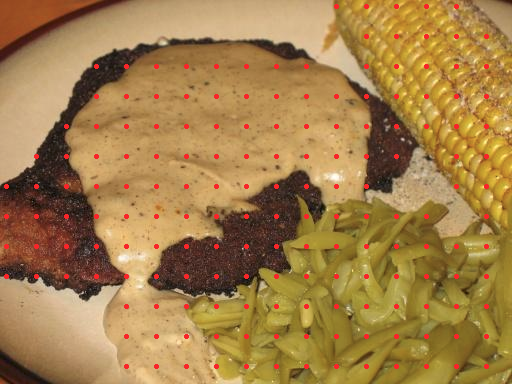
\includegraphics[width=0.45\linewidth]{figures//mobilesam/input.png}
                    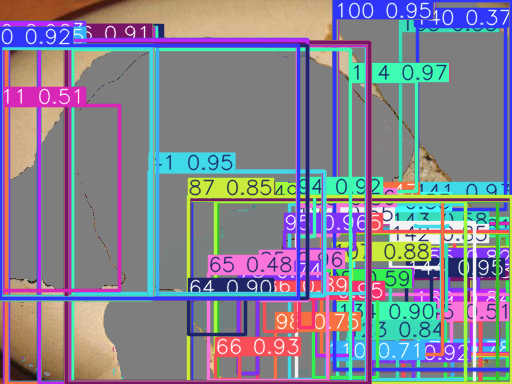
\includegraphics[width=0.45\linewidth]{figures//mobilesam/output.png}
                    % TODO: Manjkajo reference na posamezno sliko
                    \caption{Vhodna slika z mrežo točk ospredja ter izhod modela MobileSAM. MobileSAM vrne toliko instanc objektov, kolikor dobi vhodnih točk, zato za naš pristop ni ustrezen.}
                    \label{fig:mobilesam}
                \end{figure}
                
            \paragraph{FastSAM} \label{sct:fastsam}

                V nadaljevanju izvedemo eksperimente s FastSAM, kjer za poziv najprej uporabimo mrežo točk, ki označujejo zgolj ospredje. Nabor rezultatov je prikazan na sliki~\ref{fig:fastsam-points-fg}. V naslednjem preizkusu uporabimo mrežo točk za ospredje in ozadje; rezultati so na sliki~\ref{fig:fastsam-points-fg-bg}. V zadnjem eksperimentu kot poziv uporabimo okvirje, določene z enostavno pretvorbo iz odseka~\ref{sct:enostavnapretvorba}, kar je prikazano na sliki~\ref{fig:fastsam-bbox}.

                Ker FastSAM izvaja le segmentacijo brez razvrščanja objektov, so vse napovedi označene z razredom \emph{object}. Ker so vhodne slike različnih ločljivosti, razmik med točkami pa je podan v pikslih, se skupno število točk med posameznimi vzorci razlikuje.
                
                % Point based approach - foreground only
                \begin{figure}
                    \centering
                    \setlength{\tabcolsep}{2pt} % space between columns
                    \renewcommand{\arraystretch}{1} % no extra row padding
                    \begin{tabular}{@{}cccc@{}}
                    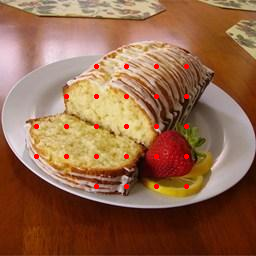
\includegraphics[width=0.24\linewidth]{figures/fastsam/points_fg/11.png} &
                    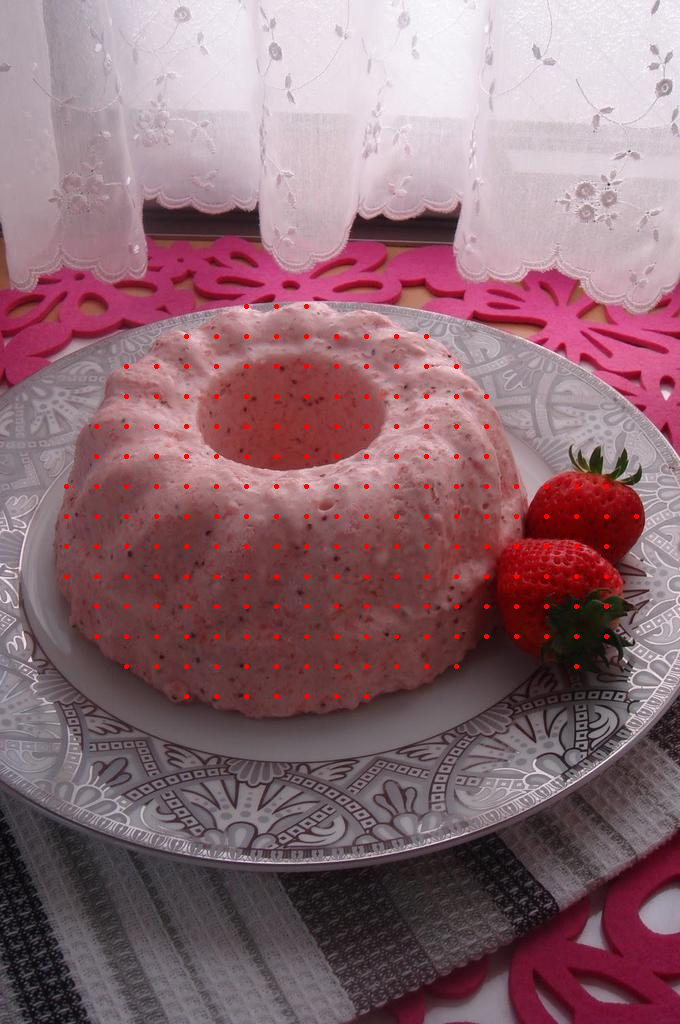
\includegraphics[trim={0.0cm 6.0cm 0.0cm 6.0cm},clip, width=0.24\linewidth]{figures/fastsam/points_fg/114.png} &
                    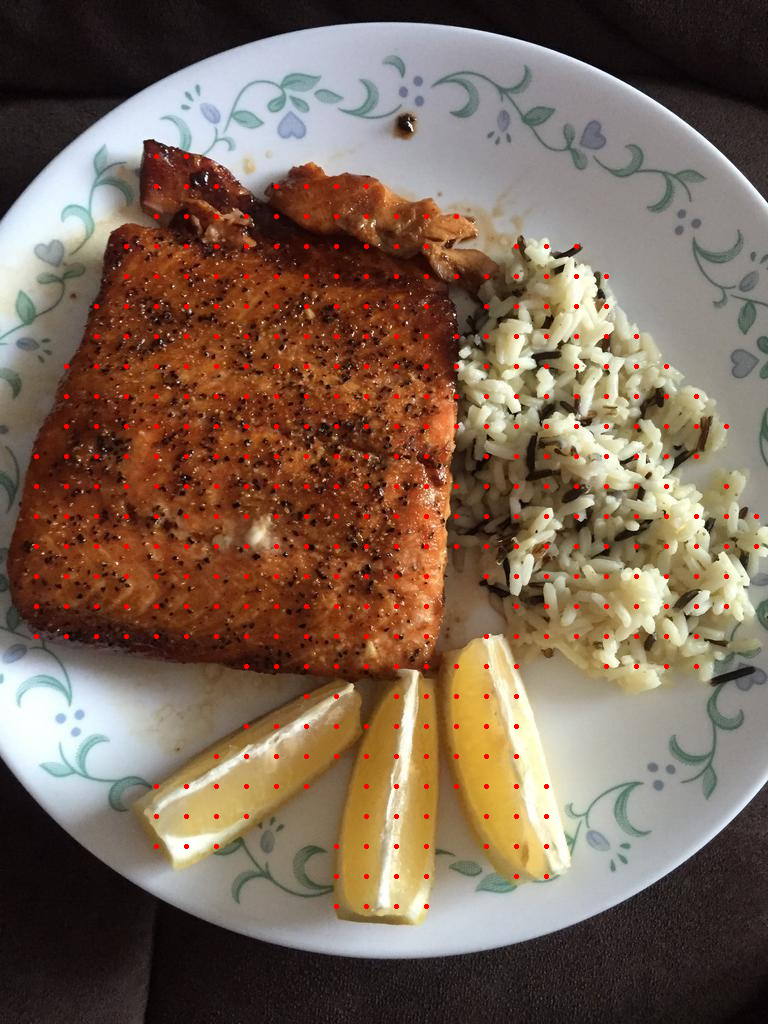
\includegraphics[trim={0.0cm 4.5cm 0.0cm 4.5cm},clip, width=0.24\linewidth]{figures/fastsam/points_fg/131.png} &
                    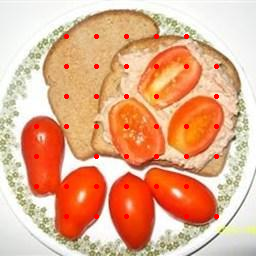
\includegraphics[width=0.24\linewidth]{figures/fastsam/points_fg/145.png} \\
                    
                    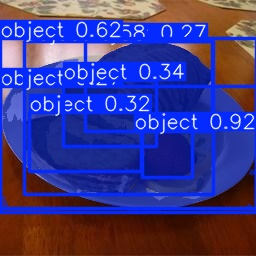
\includegraphics[width=0.24\linewidth]{figures/fastsam/points_fg/11_mask.png} &
                    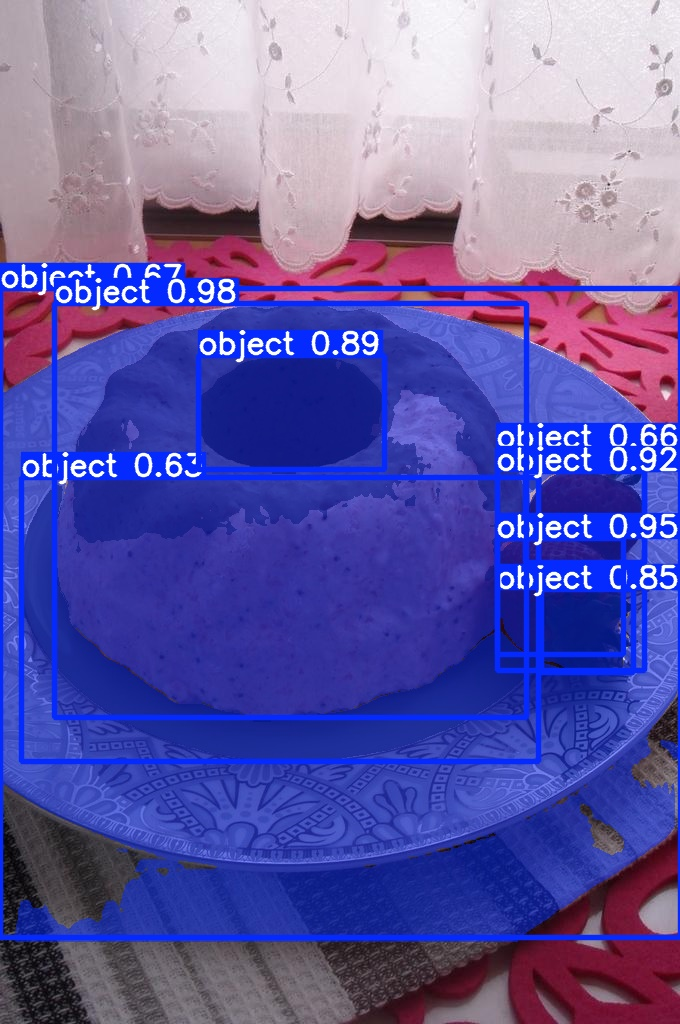
\includegraphics[trim={0.0cm 6.0cm 0.0cm 6.0cm},clip, width=0.24\linewidth]{figures/fastsam/points_fg/114_mask.png} &
                    \includegraphics[trim={0.0cm 4.5cm 0.0cm 4.5cm},clip, width=0.24\linewidth]{figures/fastsam/points_fg/131_mask.png} &
                    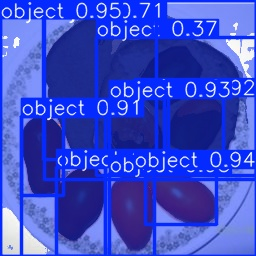
\includegraphics[width=0.24\linewidth]{figures/fastsam/points_fg/145_mask.png} \\

                    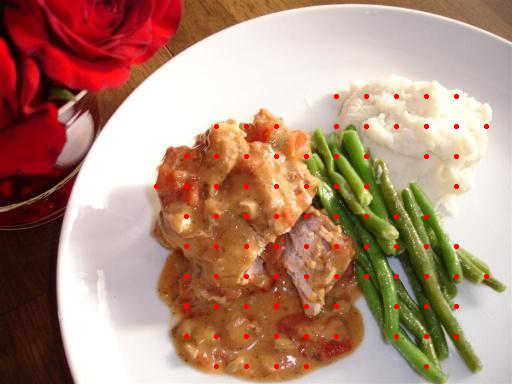
\includegraphics[width=0.24\linewidth]{figures/fastsam/points_fg/160.png} &
                    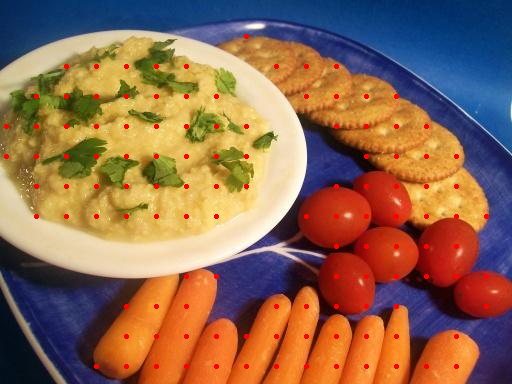
\includegraphics[width=0.24\linewidth]{figures/fastsam/points_fg/203.png} &
                    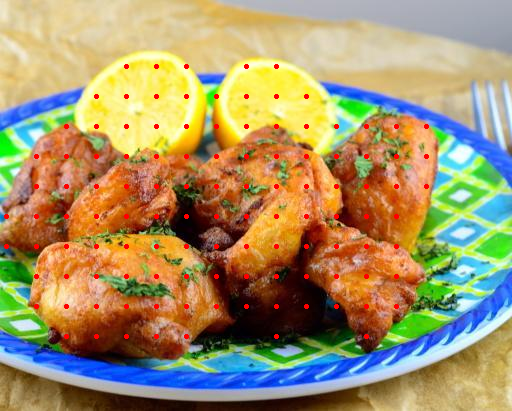
\includegraphics[trim={0.0cm 0.5cm 0.0cm 0.5cm},clip, width=0.24\linewidth]{figures/fastsam/points_fg/248.png} &
                    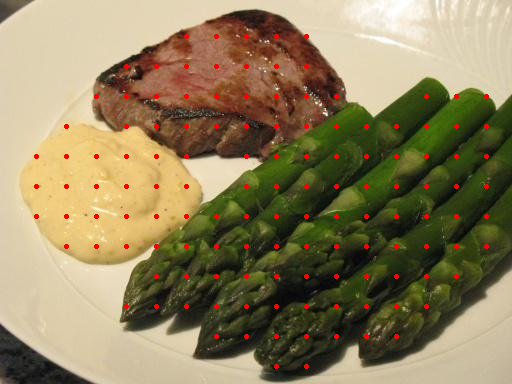
\includegraphics[width=0.24\linewidth]{figures/fastsam/points_fg/306.png} \\
                    
                    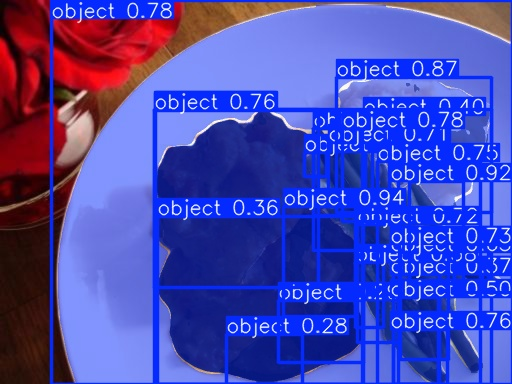
\includegraphics[width=0.24\linewidth]{figures/fastsam/points_fg/160_mask.png} &
                    \includegraphics[width=0.24\linewidth]{figures/fastsam/points_fg/203_mask.png} &
                    \includegraphics[trim={0.0cm 0.5cm 0.0cm 0.5cm},clip, width=0.24\linewidth]{figures/fastsam/points_fg/248_mask.png} &
                    \includegraphics[width=0.24\linewidth]{figures/fastsam/points_fg/306_mask.png} \\
                    \end{tabular}
                    % TODO: Oblika - katere slike sodijo skupaj?
                    \caption{Vzorec rezultatov segmentacije z modelom FastSAM in pozivom v obliki točk, ki označijo ospredje. Vrstici z modrimi maskami predstavljata izhod modela.}
                    \label{fig:fastsam-points-fg}
                \end{figure}

                % Point based approach - fg and bg
                \begin{figure}
                    \centering
                    \setlength{\tabcolsep}{2pt} % space between columns
                    \renewcommand{\arraystretch}{1} % no extra row padding
                    \begin{tabular}{@{}cccc@{}}
                    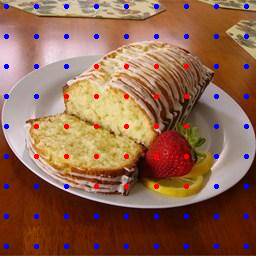
\includegraphics[width=0.24\linewidth]{figures/fastsam/points_fg_bg/11.png} &
                    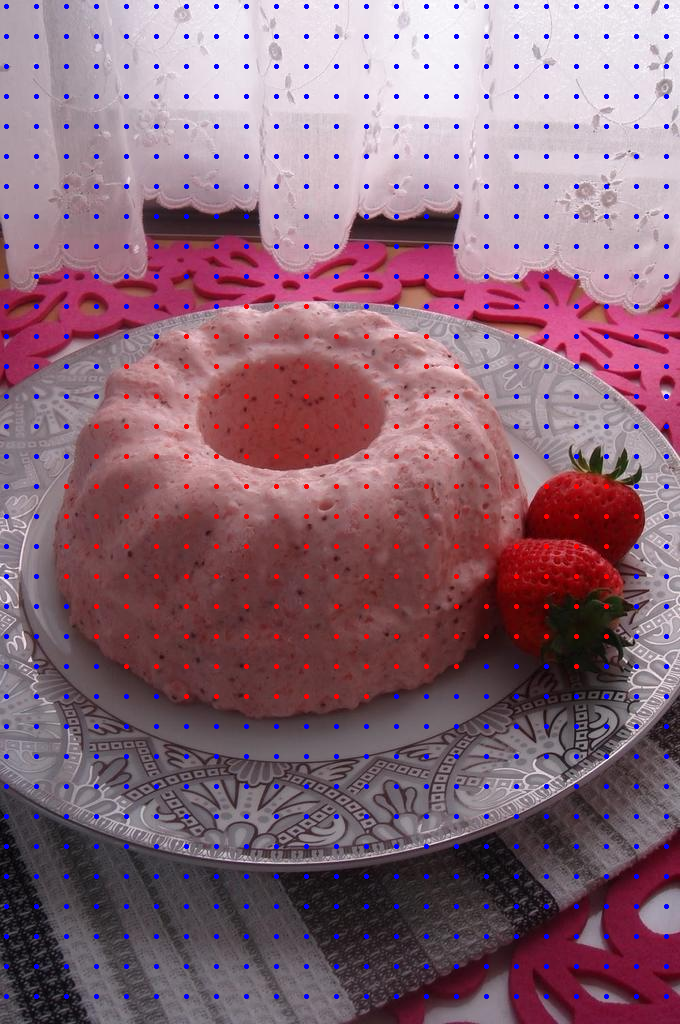
\includegraphics[trim={0.0cm 6.0cm 0.0cm 6.0cm},clip, width=0.24\linewidth]{figures/fastsam/points_fg_bg/114.png} &
                    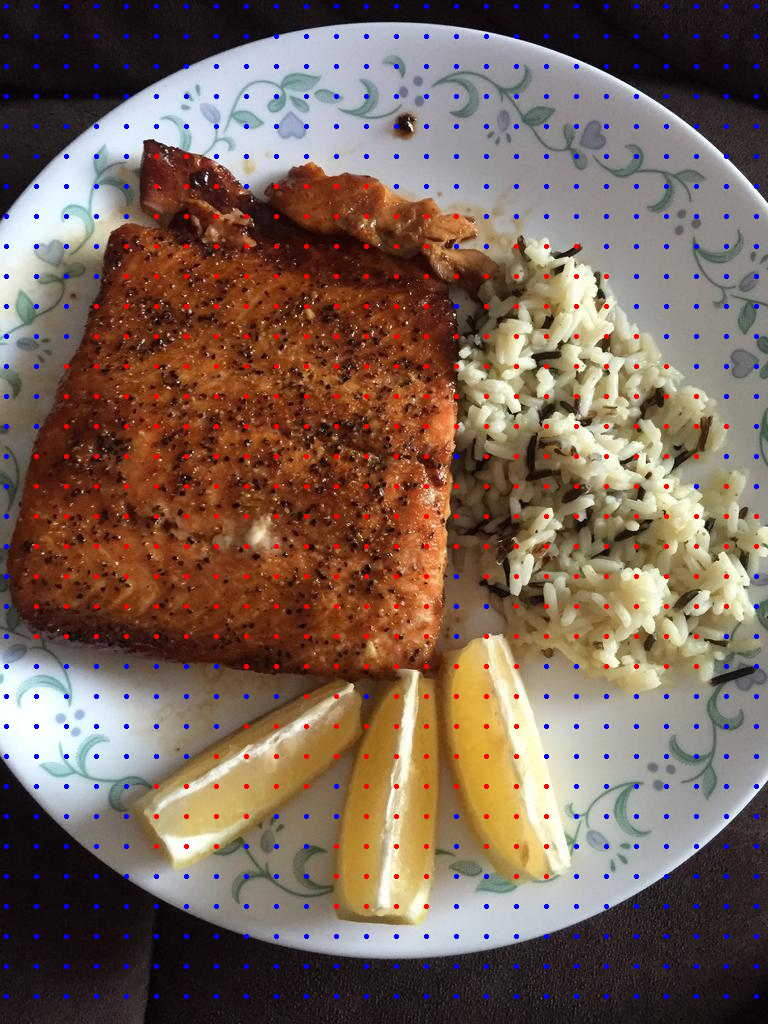
\includegraphics[trim={0.0cm 4.5cm 0.0cm 4.5cm},clip, width=0.24\linewidth]{figures/fastsam/points_fg_bg/131.png} &
                    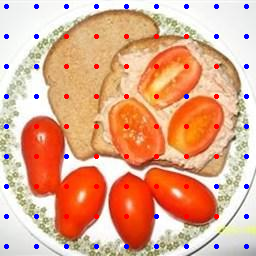
\includegraphics[width=0.24\linewidth]{figures/fastsam/points_fg_bg/145.png} \\
                    
                    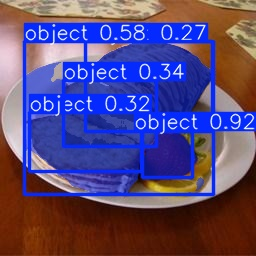
\includegraphics[width=0.24\linewidth]{figures/fastsam/points_fg_bg/11_mask.png} &
                    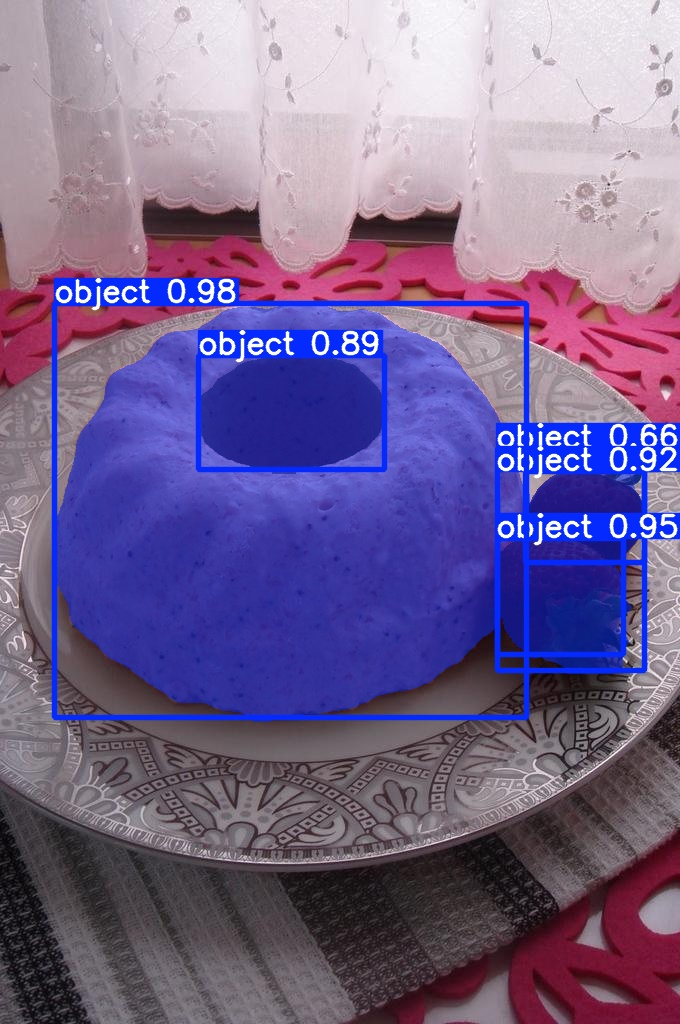
\includegraphics[trim={0.0cm 6.0cm 0.0cm 6.0cm},clip, width=0.24\linewidth]{figures/fastsam/points_fg_bg/114_mask.png} &
                    \includegraphics[trim={0.0cm 4.5cm 0.0cm 4.5cm},clip, width=0.24\linewidth]{figures/fastsam/points_fg_bg/131_mask.png} &
                    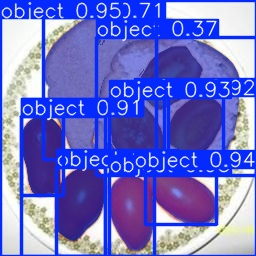
\includegraphics[width=0.24\linewidth]{figures/fastsam/points_fg_bg/145_mask.png} \\

                    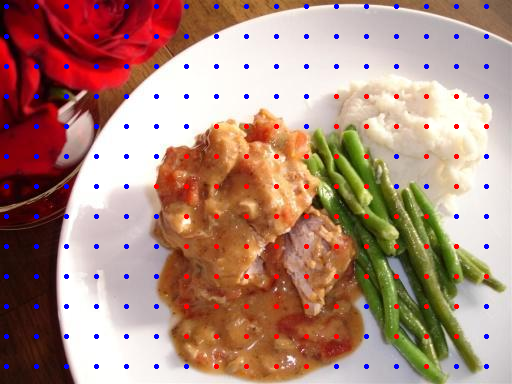
\includegraphics[width=0.24\linewidth]{figures/fastsam/points_fg_bg/160.png} &
                    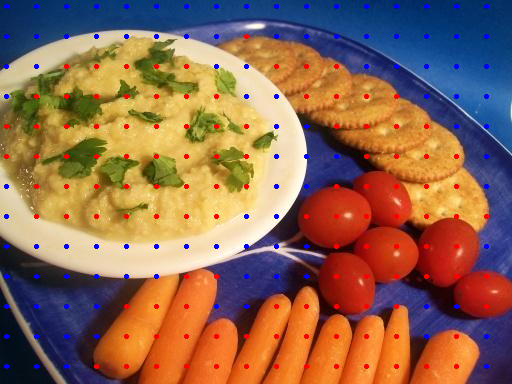
\includegraphics[width=0.24\linewidth]{figures/fastsam/points_fg_bg/203.png} &
                    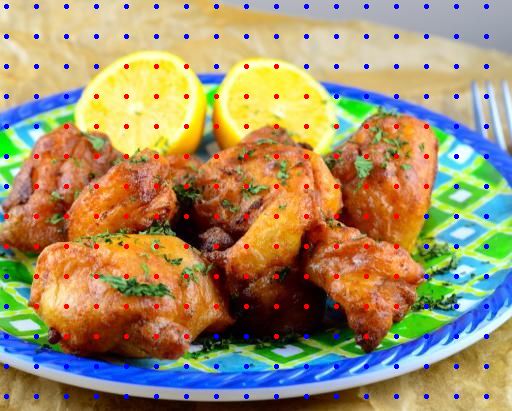
\includegraphics[trim={0.0cm 0.5cm 0.0cm 0.5cm},clip, width=0.24\linewidth]{figures/fastsam/points_fg_bg/248.png} &
                    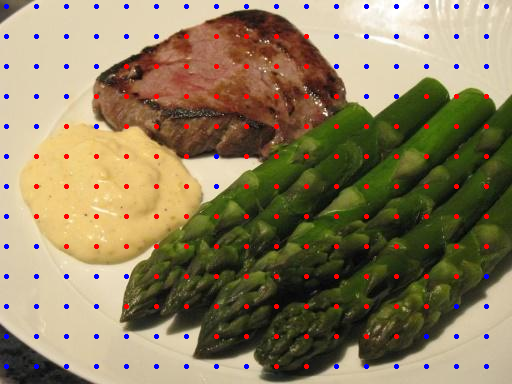
\includegraphics[width=0.24\linewidth]{figures/fastsam/points_fg_bg/306.png} \\
                    
                    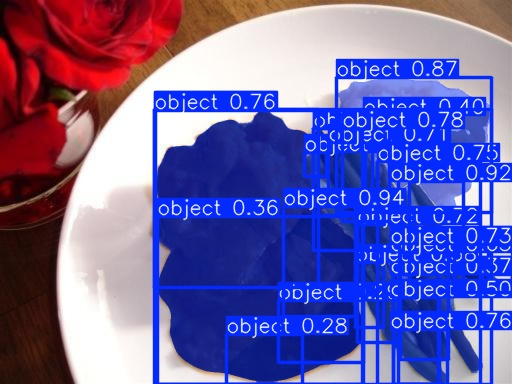
\includegraphics[width=0.24\linewidth]{figures/fastsam/points_fg_bg/160_mask.png} &
                    \includegraphics[width=0.24\linewidth]{figures/fastsam/points_fg_bg/203_mask.png} &
                    \includegraphics[trim={0.0cm 0.5cm 0.0cm 0.5cm},clip, width=0.24\linewidth]{figures/fastsam/points_fg_bg/248_mask.png} &
                    \includegraphics[width=0.24\linewidth]{figures/fastsam/points_fg_bg/306_mask.png} \\
                    \end{tabular}
                    % TODO: Oblika - katere slike sodijo skupaj?
                    \caption{Vzorec rezultatov segmentacije z modelom FastSAM in pozivom v obliki točk, ki označijo ospredje (rdeče) in ozadje (modro). Vrstici z modrimi maskami predstavljata izhod modela FastSAM.}
                    \label{fig:fastsam-points-fg-bg}
                \end{figure}

                % Bbox based approach
                \begin{figure}
                    \centering
                    \setlength{\tabcolsep}{2pt} % space between columns
                    \renewcommand{\arraystretch}{1} % no extra row padding
                    \begin{tabular}{@{}cccc@{}}
                    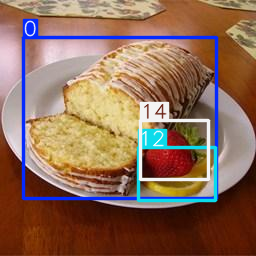
\includegraphics[width=0.24\linewidth]{figures/fastsam/bbox/11.png} &
                    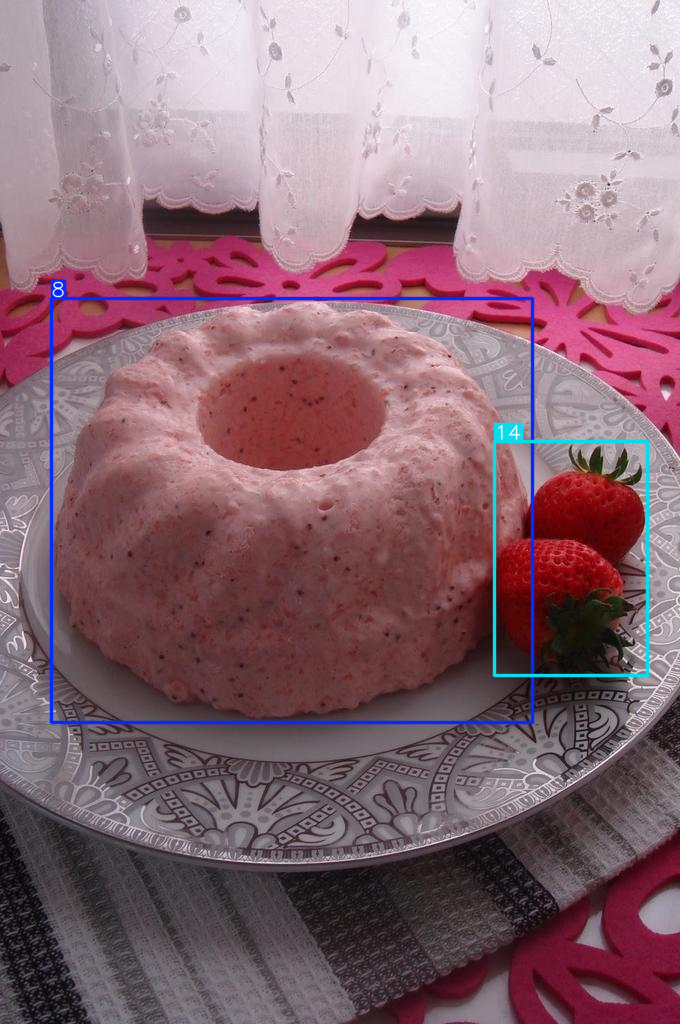
\includegraphics[trim={0.0cm 6.0cm 0.0cm 6.0cm},clip, width=0.24\linewidth]{figures/fastsam/bbox/114.png} &
                    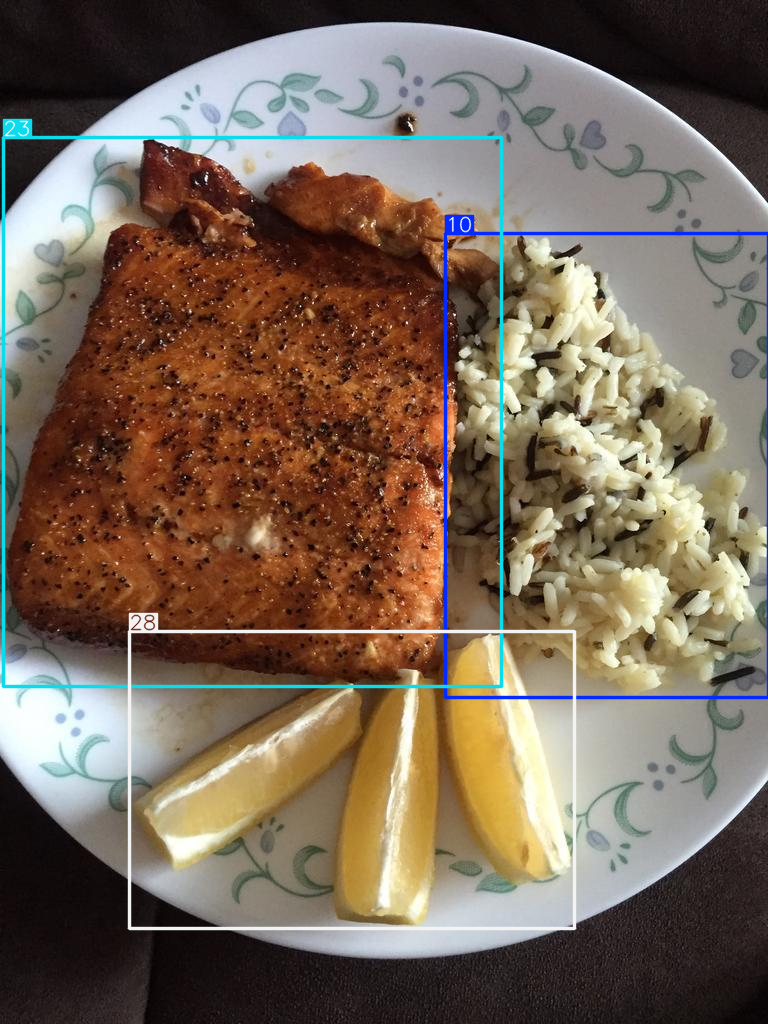
\includegraphics[trim={0.0cm 4.5cm 0.0cm 4.5cm},clip, width=0.24\linewidth]{figures/fastsam/bbox/131.png} &
                    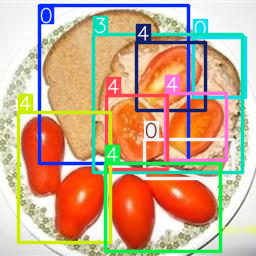
\includegraphics[width=0.24\linewidth]{figures/fastsam/bbox/145.png} \\
                    
                    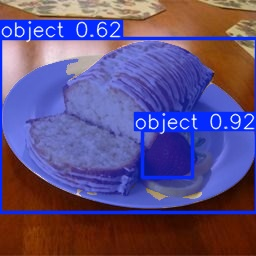
\includegraphics[width=0.24\linewidth]{figures/fastsam/bbox/11_mask.png} &
                    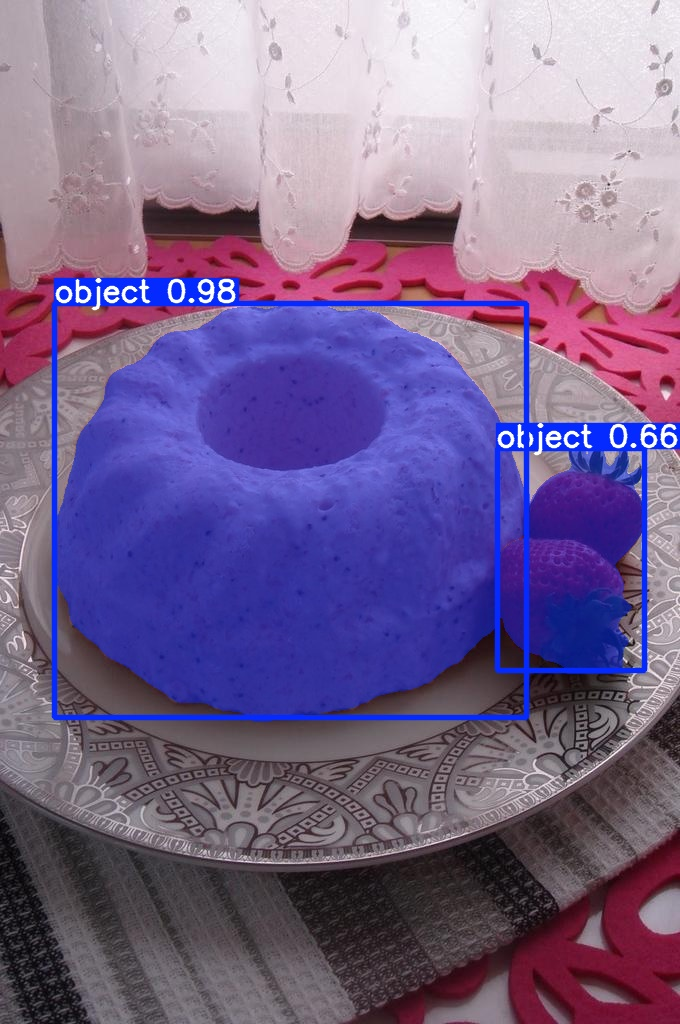
\includegraphics[trim={0.0cm 6.0cm 0.0cm 6.0cm},clip, width=0.24\linewidth]{figures/fastsam/bbox/114_mask.png} &
                    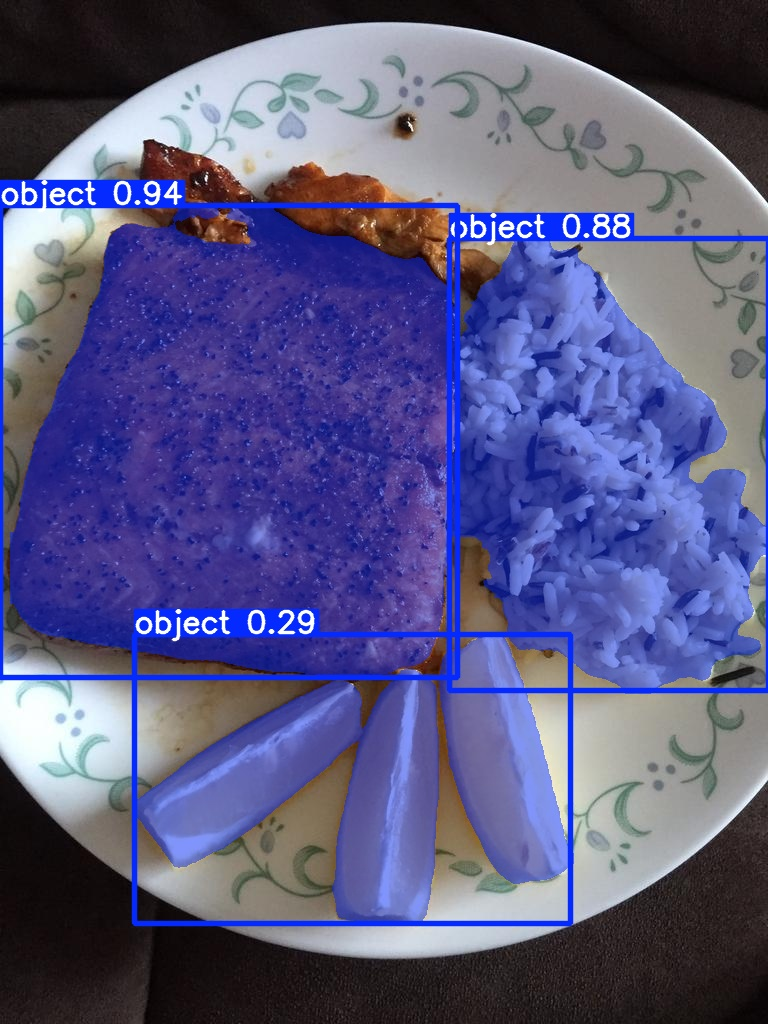
\includegraphics[trim={0.0cm 4.5cm 0.0cm 4.5cm},clip, width=0.24\linewidth]{figures/fastsam/bbox/131_mask.png} &
                    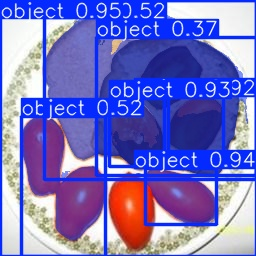
\includegraphics[width=0.24\linewidth]{figures/fastsam/bbox/145_mask.png} \\

                    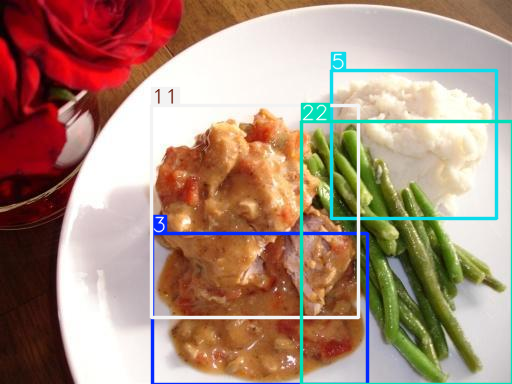
\includegraphics[width=0.24\linewidth]{figures/fastsam/bbox/160.png} &
                    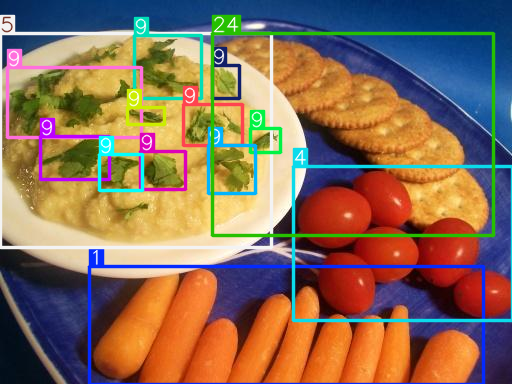
\includegraphics[width=0.24\linewidth]{figures/fastsam/bbox/203.png} &
                    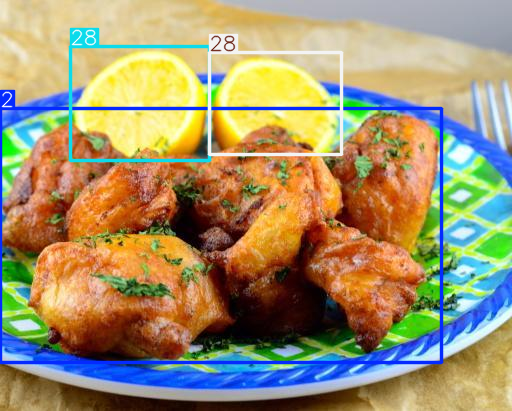
\includegraphics[trim={0.0cm 0.5cm 0.0cm 0.5cm},clip, width=0.24\linewidth]{figures/fastsam/bbox/248.png} &
                    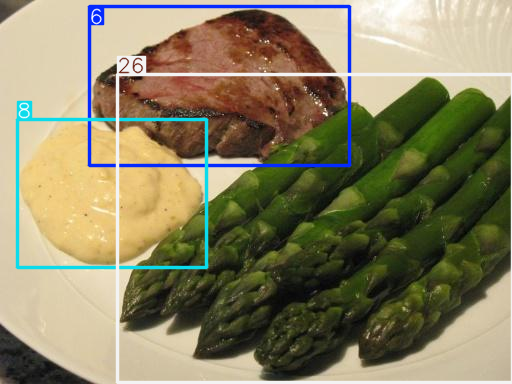
\includegraphics[width=0.24\linewidth]{figures/fastsam/bbox/306.png} \\
                    
                    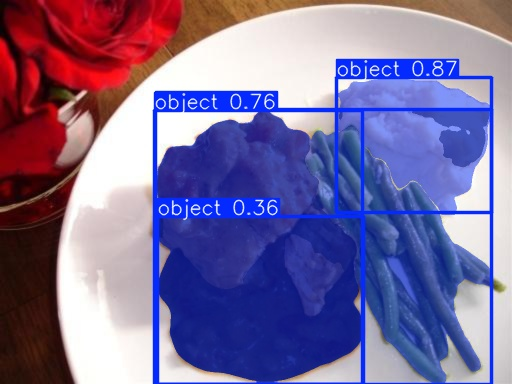
\includegraphics[width=0.24\linewidth]{figures/fastsam/bbox/160_mask.png} &
                    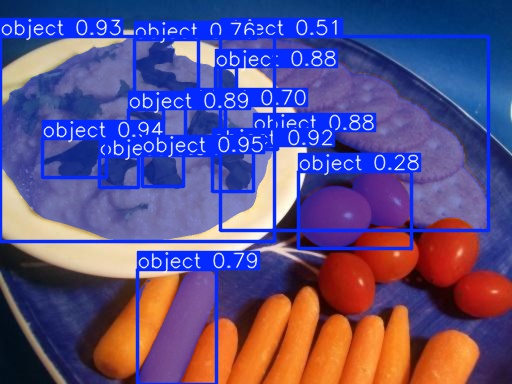
\includegraphics[width=0.24\linewidth]{figures/fastsam/bbox/203_mask.png} &
                    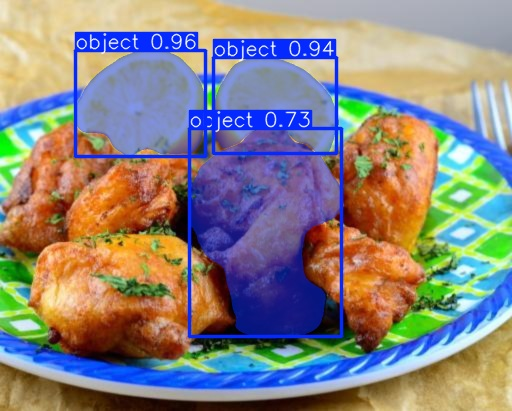
\includegraphics[trim={0.0cm 0.5cm 0.0cm 0.5cm},clip, width=0.24\linewidth]{figures/fastsam/bbox/248_mask.png} &
                    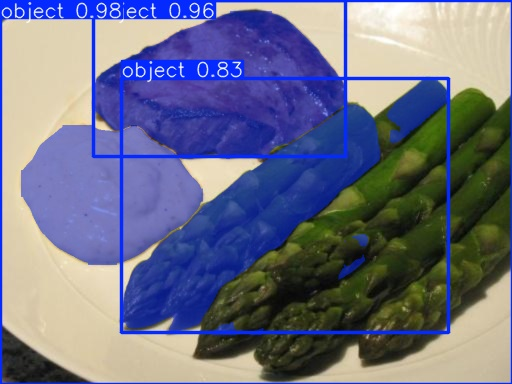
\includegraphics[width=0.24\linewidth]{figures/fastsam/bbox/306_mask.png} \\
                    \end{tabular}
                    % TODO: Oblika - katere slike sodijo skupaj?
                    \caption{Vzorec rezultatov segmentacije z modelom FastSAM in pozivom v obliki okvirjev, pridobljenih z enostavno pretvorbo iz izvirnih segmentacijskih mask. Vrstici z modrimi maskami predstavljata izhod modela FastSAM.}
                    \label{fig:fastsam-bbox}
                \end{figure}
    
    \section{Rezultati} \label{sct:rezultati}

        \subsection{Model FOMO}

        \subsection{Model YOLOv11n-seg}

        \subsection{Model SAM}

\chapter{Diskusija} \label{sct:diskusija}

    \section{Cilji in raziskovalna vprašanja}
        V tem poglavju povzamemo ugotovitve o poenostavitvi podatkovne zbirke FoodSeg103, metrikah in njihovi interpretaciji, obnašanju FOMO v primerjavi z YOLOv11-seg, izvedljivosti metod SAM ter učinku kvantizacije na izvajanje na mikrokrmilnikih.

    \section{Izbrana podatkovna zbirka in vpliv poenostavitve}
    
        Porazdelitev podatkov je izrazito problematična, saj najredkejši razredi vsebujejo le nekaj deset slik, zato zanje težko pričakujemo dobre rezultate. Dodatno težavnost prinaša narava zbirk s sestavinami hrane z visoko znotrajrazredno variabilnostjo in nizko medrazredno diferenciacijo. Tudi najboljši objavljeni pristopi na tej zbirki praviloma dosegajo okoli 50~\% mIoU, kar potrjuje zahtevnost problema. V naših poskusih z YOLOv11x-seg smo dosegli 28{,}4~\% mIoU. V kontekstu omejitev mikrokrmilniških modelov to nakazuje, da je zbirka v izvorni obliki za naš primer uporabe zelo zahtevna in precej neustrezna.
    
        Zato smo se lotili poenostavitve zbirke. Poenostavitev je skrajšala rep porazdelitve in povečala povprečno število primerov na razred, hkrati pa znižala pokritost redkih razredov in skupni obseg podatkov. Nastane jasen kompromis: premalo odstranjevanja pusti premalo podatkov na repu in slabše rezultate na teh razredih; preveč odstranjevanja zmanjša nabor do mere, ko kakovostno učenje ni več mogoče. V različici s 30 razredi je povprečno število slik na razred \(322{,}9 \pm 188{,}5\); dodatno se učinkovita količina učnih podatkov zmanjša, ker del nabora namenimo validaciji in testu.
    
        Če bi delo nadaljevali z zbirko FoodSeg103, bi bilo smiselno razmisliti o drugačnem načinu poenostavitve. V odseku~\ref{sct:foodseg103-poenostavitev} smo obravnavali več pristopov. Prepisovanje mask neželenih razredov v ozadje se ne izkaže kot ustrezno, saj poveča varianco ozadja, ki pogosto vsebuje segmente hrane, in s tem oteži učenje odločitvenih mej. Perspektivnejša možnost je združevanje sorodnih razredov v širše, semantično koherentne kategorije, kar ohranja velikost nabora in znižuje neuravnoteženost, vendar zahteva premišljeno definicijo nadrazredov in dodatno urejanje oznak.

    \section{Ustreznost izbranih metrik}

        Izbor metrik na ravni pikslov in metrik prisotnosti razredov daje vpogled tako v lokalizirano klasifikacijo kot v uporabnost za končni cilj. Metrika mIoU do neke mere omogoča primerljivost z literaturo. Razred ozadje pri metrikah praviloma izključimo, ker nas zanimajo sestavine. Pri metrikah prisotnosti razredov je ozadje še posebej nerelevantno, saj je prisotno na vsakem vzorcu.
        
        Uporaba metrike mIoU je v našem okolju problematična zaradi zelo nizke ločljivosti izhodnih mask. Če objekt na maski zavzame le nekaj pikslov, je vrednost IoU izrazito nezvezna in lahko preskakuje med skrajnimi vrednostmi. To oteži zanesljivo primerjavo med modeli, zlasti pri majhnih in delno vidnih objektih. Metrika je bolj relevantna za primerjavo modela YOLOv11-seg, ker ima tista izhodna maska višjo ločljivost.
        
        Metrike na ravni pikslov \(F1_p\) povedo, kako model lokalizira razrede, kar ni neposreden cilj naloge, je pa koristno pri analizi napak. Z njimi lažje prepoznamo, katere razrede model zamenjuje med seboj, saj je za tak vpogled potrebna tudi informacija o lokaciji. Vsekakor pa jo težko uporabimo za primerjavo z ostalimi deli.
        
        Metrika prisotnosti razredov \(F1_r\) je v kontekstu naše naloge najbolj relevantna. Občutljiva je na prag minimalnega števila zaplat \(\nu\), ki je izbran hevristično, in opira se na naknadno obdelavo, ki preoblikuje izhod modela. Ta dodatna kompleksnost lahko slabša stabilnost rezultata. Ena od možnosti za izboljšavo je zamenjava naknadne obdelave z gosto izhodno plastjo in obravnava modela kot večoznačnega klasifikatorja prisotnosti razredov. Tak pristop bi bolje sledil cilju naloge, a modela ne bi neposredno silil v pravilno lokalizacijo.
    
    \section{Ključne ugotovitve in omejitve modela FOMO}
    
        FOMO omogoča izredno hitro učenje in nizko računsko zahtevnost, vendar je omejen z nizkoločljivostnim izhodom in majhnim receptivnim poljem.

        % Komentar na eksperimente
        
        \subsection{Učenje na izvirni FoodSeg103 zbirki}
        
            Najprej smo v odseku~\ref{sct:ucenje-na-izvirnem-datasetu} model FOMO učili na izvirni, nepoenostavljeni zbirki FoodSeg103, rezultati pa so zbrani v tabeli~\ref{tab:experiment_full_foodseg103_dataset_table}. Po metriki mIoU je dosežena uspešnost v primerjavi z najboljšimi pristopi zanemarljiva. K temu verjetno prispevajo majhna kapaciteta modela, nizkoločljivostna izhodna maska (npr. \(8 \times 8\) ali \(16 \times 16\)), nestabilnost IoU pri zelo majhnih objektih in sama zahtevnost podatkovne zbirke.
            
            Rezultati \(F1_r\)  so zelo slabi. Konfuzijska matrika kaže vedenje, ki je blizu naključnemu ugibanju. Posebej problematični so zelo redki razredi, kot je \emph{kelp}, za katere konfuzijska matrika nakazuje, da imajo praktično nič referenčnih pikslov. Pri nizki izhodni ločljivosti se ti razredi pogosto izgubijo pri zmanjševanju maske, kar pomeni, da predprocesiranje pomembno spremeni statistične lastnosti podatkov.
            
            Uniformno uteževanje nepoenostavljene podatkovne zbirke je dalo malenkost boljše rezultate, kot pa uteževanje po frekvenci razredov.
            Slednje se je po analizi izkazalo za problematično. Najredkejši razredi dobijo zelo visoke uteži, tudi do faktorja \(\sim 4000\), medtem ko je ozadje uteženo z \(1\). Na sliki~\ref{fig:experiment_full_foodseg103_dataset_loss} je razvidno, da pri uteževanju po frekvenci validacijska krivulja hitreje kaže znake prenaučenja. Deloma je to pričakovano, saj večje uteži pospešijo učenje teh razredov. Dodatno pa na obliko krivulje vpliva sama definicija kriterijske funkcije. V odseku~\ref{sct:fomo-ucenje} smo opisali, da je izgubna funkcija utežena po razredih, zato imajo napake visoko uteženih in hkrati slabo zastopanih razredov nesorazmerno velik vpliv na skupno izgubo, zaradi česar se prenaučenje teh razredov pokaže prej.
            

        \subsection{Učenje na poenostavljeni zbirki}
            
            Zaradi izrazito slabih rezultatov in problematike zelo redkih razredov smo zato zbirko poenostavili in odstranili najslabše zastopane razrede. Eksperimenti so predstavljeni v odseku~\ref{sct:fomo-simplified-experiments}.

            % Primerjava rezultatov z nepoenostavljeno zbirko. A so rezultati uporabni?
            V tabeli~\ref{tab:experiment_simplified_foodseg103_dataset_table} prikažemo, da dosežemo do 24 odstotkov boljše rezultate v metriki $F1_r$ v primerjavi z eksperimenti na nepoenostavljeni zbirki. Vsekakor so rezultati izrazito boljši, vendar so še vedno prenizki, da bi lahko rekli, da model zanesljivo reši podatkovno zbirko.
            % Komentar na mIoU, da ga lahko primerjamo samo z našim YOLO eksperimentom, ker smo spremenili dataset.
            Tudi metriki $F1_p$ in mIoU se izrazito izboljšata za 19 oziroma 12 odstotkov, vendar so vrednosti še vedno prenizke za zanesljivo delovanje.

            % Primerjava različnih načinov uteževanja.
            Uteževanje v tem primeru nima tako bistvenega vpliva kot pri nepoenostavljeni zbirki. Razlika v metrikah znaša največ en odstotek.
            % Komentar na grafe kriterijske funkcije, ni več take razlike med različnimi uteževanji, ker ni več razredov z izjemno velikimi utežmi
            Tudi kriterijski funkciji na sliki~\ref{fig:experiment_simplified_foodseg103_dataset_loss} sta si precej bolj podobni, saj je distribucija razredov precej bolj enakomerna, tako da ni več razredov z izjemno velikimi utežmi, ki bi potencialno destabilizirali učenje.

        \subsection{Učenje na poenostavljeni zbirki}

            Zaradi slabih rezultatov na izvirni zbirki in izrazitega vpliva zelo redkih razredov smo zbirko poenostavili ter odstranili najslabše zastopane razrede. Eksperimente s poenostavljeno različico predstavljamo v odseku~\ref{sct:fomo-simplified-experiments}.
            
            V tabeli~\ref{tab:experiment_simplified_foodseg103_dataset_table} pokažemo, da se metrika \(F1_r\) glede na učenje na izvirni zbirki izboljša tudi za 24~\%. Rezultati so občutno boljši, vendar še vedno niso dovolj visoki za zanesljivo uporabo modela. Metriki \(F1_p\) in mIoU se prav tako izboljšata, in sicer za približno 19~\% oziroma 12~\%. Pri mIoU opozorimo, da je neposredna primerjava z literaturo neustrezna, saj je zbirka precej poenostavljena. Smiselna je predvsem primerjava z našimi lastnimi referencami na YOLOv11-seg na isti različici podatkov.
            
            Vpliv uteževanja razredov je po poenostavitvi zbirke bistveno manjši. Razlike v metrikah so največ okoli en odstotek. Krivulji kriterijske funkcije sta si pri različnih uteževanjih precej podobni, ker je porazdelitev razredov bolj enakomerna in ni več razredov z izjemno velikimi utežmi, ki bi potencialno destabilizirale učenje. Poenostavitev torej pomaga pri stabilnosti in doseženih metrikah, a rešuje zgolj problem neuravnovešenosti podatkovne zbirke, ostale omejitve pa ostajajo.
    
            % TODO
            % Metrike kažejo praktično isti performance. Kaj pa konfuzijske matrike? Je uteževanje na podlagi frekvence boljše? Je to morda posledica neuglašenega parametra \tau?

        % Primerjava resolucij
        \subsection{Primerjava različnih kombinacij resolucij}
            V odseku~\ref{sct:primerjava-resolucij} primerjamo različne kombinacije vhodne in izhodne ločljivosti, saj te skupaj s faktorjem zmanjšanja močno vplivajo na delovanje modela.

            Najboljše vrednosti \(F1_p\) in mIoU dosežemo pri kombinaciji \mbox{\(128 \times 128 \rightarrow 16 \times 16\)}. Po metriki \(F1_r\) je ta nastavitev primerljiva z \mbox{\(96 \times 96 \rightarrow 12 \times 12\)}. Obe navedeni nastavitvi sta se izkazali kot zanesljivi, zadovoljive rezultate pa daje tudi kombinacija \mbox{\(128 \times 128 \rightarrow 8 \times 8\)}. Najslabše rezultate opazimo pri najmanjši izhodni ločljivosti \mbox{\(6 \times 6\)}. Tudi pretirano velike izhodne ločljivosti se pri dani kapaciteti modela niso izkazale kot koristne.

            Nizke izhodne ločljivosti so lahko problematične, ker se pri zmanjševanju ločljivosti maske majhni objekti pogosto izgubijo, informacija v posamezni zaplati pa postane preveč groba, kar zniža kakovost učinkovitih anotacij in oteži učenje.
            % Mogoče je to odvisno od izhodne resolucije, ampak težko argumentiram.
            Na podlagi teh ugotovitev smo se v nadaljevanju omejili na ločljivost \mbox{\(128 \times 128 \rightarrow 16 \times 16\)}.

        \subsection{Primerjava strategij učenja}
        
            V odseku~\ref{sct:primerjava-strategij-ucenja} primerjamo učenje celotnega modela (\emph{end-to-end}) z učenjem zgolj glave z zamrznjeno hrbtenico. Hrbtenica je v obeh primerih prednaučena na zbirki ImageNet. Iz rezultatov v tabeli~\ref{tab:strategije-ucenja} je razvidno, da \emph{end-to-end} učenje doseže občutno boljše vrednosti metrik kakor učenje samo glave. Razlogov je lahko več. Eden izmed potencialnih razlogov je, da prednaučene uteži na ImageNet niso domensko povsem ustrezne za razpoznavo sestavin hrane, zaradi česar je prenos znanja omejen. Mogoče bi bila bolj primerna hrbtenica, prednaučena na zbirki, kot recimo Food-101, ki poglavitno vsebuje slike hrane. Drug razlog bi lahko bil, da pri gradnji FOMO hrbtenice MobileNetV2 preveč odrežemo, zaradi tako velike arhitekturne spremembe pa prednaučene uteži niso več dovolj relevantne.

        \subsection{Specializirani modeli po posameznih razredih}

            Izbrani model je v primerjavi s SOTA pristopi zelo majhen, zato smo v odseku~\ref{sct:specializirani-modeli} preizkusili idejo specializacije: namesto enega modela, ki pokriva vse razrede, učimo ločen model za vsak posamezen razred. Za referenco uporabimo FOMO iz odseka~\ref{sct:fomo-simplified-experiments} z enakomernim uteževanjem ter poročamo metriki \(F1_r\) in \(F1_p\) brez povprečenja, torej po razredih. Eksperiment zavoljo enostavnosti izvedemo na zgolj treh razredih: \emph{broccoli} (najbolje rešen v referenci), \emph{chicken duck} in \emph{cake} (najslabše rešen v referenci).
            
            Rezultati v tabeli~\ref{tab:moe-results} ne kažejo prednosti specializiranih modelov pred referenco. Pri \emph{chicken duck} se \(F1_p\) nekoliko izboljša, a \(F1_r\) pade; \emph{broccoli} ostane približno na ravni reference, \emph{cake} pa ostaja izrazito slabo rešen.
            
            Verjeten razlog je priprava podatkov: z združevanjem vseh drugih razredov v ozadje povečamo varianco razreda ozadje, ki tako pogosto vsebuje dele hrane. Model zato še vedno rešuje težko diskriminacijsko nalogo “ciljni razred proti raznolikemu ozadju”, kjer se mora še vedno močno zanašati na teksturo in barvo po zaplatah. Ob uporabljeni kapaciteti (\(\alpha=1{,}0\)) specializacija sama po sebi tako ne zniža zahtevnosti naloge dovolj, da bi prinesla opazno izboljšanje.

        \subsection{Parameter $\alpha$}

            V odseku~\ref{sct:kvantizacija} preverimo tudi vpliv parametra $\alpha$ na dosežene metrike. $\alpha$ je parameter širine modela, in je specifičen za MobileNetV2. Načeloma vpliva na kapaciteto modela, saj z dodajanjem parametrov povečujemo opisno zmožnost modela. V tabeli~\ref{tab:alpha-perf-ptq} so prikazane dosežene metrike za tri izbrane vrednosti $\alpha$. Kot je pričakovano, večja vrednost $\alpha$ in posledično večja kapaciteta parametrov vodi k znatno boljšim rezultatom v metrikah. 
            To nakazuje, da je kapaciteta do neke mere ena izmed omejitev, ki jih srečujemo pri tem problemu, in da bi povečanje kapacitete potencialno pomenilo doseganje boljših rezultatov.

        \subsection{Kritična ocena modela} \label{sct:fomo-diskusija-kriticen-pogled}
            
            Model se v promocijskih materialih pogosto predstavi kot zelo nov pristop~\cite{src:fomodocs}, vendar iz vidika znanstvene primerljivosti ostajajo odprta vprašanja. Manjkajo sistematične primerjave na uveljavljenih zbirkah in z uveljavljenimi metrikami, dodatno pa izhod v obliki centroidov oteži neposredno primerjavo s klasičnimi detekcijskimi metrikami. Glavna praktična prednost je preprostost uporabe v ekosistemu Edge Impulse (enostaven zajem in obdelava podatkov ter izvoz na robne naprave), ne pa nujno preboj v samem modeliranju. Tudi nekatera druga dela so kritična glede modela FOMO~\cite{src:boyle2024dsort}.
            
            % Kaj pravijo drugi viri o FOMO (brez citatov tu, samo napotek kam kasneje v referencah); poudari, da je glavna prednost enostavnost uporabe.
            
            Arhitekturno je model omejen z majhnim receptivnim poljem in nizkoločljivostnim izhodom. Posamezne zaplate se klasificirajo skoraj neodvisno, zato se model primarno opira na lokalne teksturne in barvne pozive znotraj zaplate. To pojasni dobre rezultate pri razredih z izrazito teksturo in barvo (npr.\ \emph{broccoli}) ter težave pri razredih z vizualno podobnimi teksturami, kjer je za razlikovanje potrebna informacija oblike (npr.\ \emph{pork} proti \emph{chicken duck}). Kratka hrbtenica dodatno omeji kapaciteto: v našem izrezu ohranimo le 4{,}8~\% parametrov in 36{,}6~\% plasti iz izvornega MobileNetV2 (glej~\ref{sct:fomo-ekstraktor-znacilk}). Prednost tako majhne arhitekture je sicer lahka izvedba na robnih napravah, slabost pa je nižja zgornja meja natančnosti. Rezultati z različnimi nastavitvami \(\alpha\) (glej~\ref{sct:kvantizacija}) kažejo, da dodatna kapaciteta praviloma pomaga in je potencialna smer nadgradnje modela. To lahko primarno dosežemo s povečanjem parametra $\alpha$ ali pa z arhitekturnimi spremembami hrbtenice.
            
            Pomemben vpliv ima tudi naknadna obdelava izhoda. Zasnova kot nizkoločljivostna segmentacija model sili v pravilno lokalizacijo, toda prisotnost razredov na sliki izrazimo šele v naknadni obdelavi, pri čemer se del informacije zavrže in temelji na pravilih in dveh hiperparametrih \(\tau\) in \(\nu\). Ta nista optimizirana med učenjem, temveč izbrana hevristično. Alternativno bi lahko namesto tega uporabili gosto povezano izhodno plast in model obravnavali kot večoznačni klasifikator prisotnosti razredov; parametri bi se učili skupaj z ostalimi utežmi. Kompromis takšnega pristopa je izguba neposredne zahteve po lokalizaciji. Možna vmesna rešitev je dvostopenjski postopek: najprej naučiti nizkoločljivostno segmentacijo, nato hrbtenico zamrzniti ter dodati in naučiti gosto plast, ki neposredno napove prisotne razrede. Tako bi ohranili naučeno lokalizacijsko znanje, hkrati pa bi metrika prisotnosti postala del učnega cilja, ne naknadne obdelave.
    
    \section{Primerjava z YOLOv11-seg}
        
        S tem eksperimentom smo pridobili lastno referenco o tem, kako dobro večji sodoben segmentacijski model reši FoodSeg103, ter dodatno potrditev zahtevnosti naloge. Rezultati so zbrani v tabeli~\ref{tab:yolo11-iou-table}. YOLOv11-seg nudi višjo ločljivost mask in doseže višje mIoU, vendar je bistveno večji in zahtevnejši za izvajanje. FOMO ostaja primernejši za preprostejše naloge in tam, kjer sta ključni nizka latenca in majhen pomnilniški odtis.
        
        \paragraph{Primerjava s FOMO.}
        V primerjavi s FOMO (tabele~\ref{tab:experiment_full_foodseg103_dataset_table} in~\ref{tab:experiment_simplified_foodseg103_dataset_table}) opazimo izrazit porast mIoU, kar potrjuje, da YOLOv11-seg v tem pogledu deluje bolje, kar je glede na velikost in arhitekturno zasnovo pričakovano. Poenostavljena različica zbirke FoodSeg103 je za YOLO očitno lažja od izvirne, kar je skladno tudi z opažanji pri FOMO. Kljub temu absolutne mIoU vrednosti ostajajo zmerne, kar ponovno kaže na zahtevnost izbrane zbirke.
        
        \paragraph{\emph{Nano} proti \emph{extra large}.}
        Iz histogramov na sliki~\ref{fig:yolo11-bars} je razvidno, kateri razredi so problematični za YOLO modele. Manj pogosti razredi so izrazito slabše rešeni, pri čemer razlika med različicama \emph{nano} in \emph{extra large} pride najbolj do izraza prav na repu porazdelitve. Tabela~\ref{tab:yolo11-iou-table} in slika~\ref{fig:yolo11-bars} dodatno nakazujeta, da poenostavitev nabora pomaga: odstranitev najredkejših razredov dvigne mIoU. Na podlagi porazdelitve IoU po razredih histogram okvirno nakazuje, da bi bila lahko potrebna poenostavitev celo manj obsežna (npr. odstranitev približno 30 najslabše zastopanih razredov), vendar tak sklep zahteva dodatne preizkuse.
        
        \paragraph{Opomba o kvantizaciji in izvozu.}
        Okolje Ultralytics dobro podpira kvantizacijo in izvoz v format TFLite, vendar se je pri segmentacijskem modelu izkazalo, da pretvorba ni popolna: izvajanje prek STMCube.AI MCU okolja je bilo problematično, okolje Tensorflow Lite Micro prav tako, saj slednje še ne podpira hibridnih modelov (mešanih podatkovnih tipov). Glede na število parametrov lahko ocenimo, da bi kvantizirana \emph{nano} izvedba (\textit{int8} uteži) imela najmanj približno \(2{,}8\)\ MB uteži; dejanska velikost in poraba RAM pa sta odvisni od vmesnih tenzorjev in podpore operacij. \textit{Float32} izvedbo smo lahko zagnali in izmerili porabo, vendar se točni podatki razlikujejo glede na okolje in različico orodij, zato jih v tem poglavju ne navajamo.
        % TODO: Mogoče probaj dejansko izmerit
        Ugotovitev ostaja, da novejši segmentacijski modeli z optimizacijami niso nujno daleč od praktične uporabe na robnih napravah, saj omejitve vse bolj izvirajo iz podpore orodij in operatorjev, ne zgolj iz velikosti modela.

    \section{Vloga metod SAM}
    
        V odseku~\ref{sct:rezultati-sam} smo predstavili eksperimente z MobileSAM in FastSAM, kjer smo kvalitativno ocenjevali, v kolikšni meri bi lahko s pozivi pretvorili semantične segmentacijske maske najprej v instančne, nato pa še v okvirje za učenje detekcijskih modelov. Preizkusili smo različne oblike pozivov (mreža točk ospredja, mreža točk ospredja in ozadja, ter okvirji) in rezultate primerjali na izbranih primerih.
        
        Ugotovitev je, da so metode SAM uporabne predvsem kot generatorji predlogov segmentov, ki lahko pospešijo ročno anotiranje ali popravljanje anotacij. Težko pa iz njih brez dodatnega preverjanja in ročnega posega dobimo konsistentne, kakovostne instančne maske. SAM torej ni \emph{end-to-end} rešitev za našo nalogo, lahko pa poenostavi najzahtevnejši del - risanje mask na objekt.
        
        \paragraph{MobileSAM.}
        MobileSAM se v našem kontekstu ne izkaže kot primeren za pozive z mrežo točk, saj vrne toliko instanc, kolikor je vhodnih točk. To je razvidno na sliki~\ref{fig:mobilesam}. Ker želimo, da metoda sama določi tudi število instanc, je tak izhod povsem neprimeren za naš cilj.
        
        \paragraph{FastSAM.}
        FastSAM nima omenjene omejitve. Rezultati z mrežo zgolj točk ospredja so prikazani na sliki~\ref{fig:fastsam-points-fg}, z dodanimi točkami ozadja pa na sliki~\ref{fig:fastsam-points-fg-bg}. V preprostih prizorih, kjer so objekti jasno ločeni, doseže sprejemljive segmente, v kompleksnejših pa pogosto odpove. Dodajanje točk ozadja praviloma izboljša rezultate, saj model dobi jasnejšo informacijo, kaj naj obravnava kot ozadje; posledično je na sliki~\ref{fig:fastsam-points-fg-bg} manj napak (npr. segmentirani krožniki, ki bi morali biti del ozadja). Preverili smo tudi pozive v obliki okvirjev (slika~\ref{fig:fastsam-bbox}); ta pristop se je izkazal za manj ustreznega, kar je pričakovano, saj okvir nosi manj informacij kot mreža točk, in številni objekti ostanejo nesegmentirani.
        
        \paragraph{Praktična uporabnost.} % Overall sentiment
        V praksi FastSAM marsikdaj generira slabše okvirje, kot jih že imamo; včasih so boljši pozivi s točkami, drugič z okvirji. Ključna pomanjkljivost je, da pri uporabi FastSAM izgubimo informacijo o razredu objekta, zato tak potek dela za naš namen ni posebej koristen in z njim nismo nadaljevali.
        
        \paragraph{Težava definicije objektov.}
        Še bolj bistvena, temeljna ovira je definicija, kaj šteje kot posamezen objekt. Pri nalogah, kot so “osebe” ali “vozila”, je ta odločitev običajno jasnejša; pri sestavinah hrane je pogosto nejasno, ali je ustrezneje združiti več delov v eno instanco ali jih obravnavati ločeno. To je razvidno že na rezultatih s točkami ospredja in ozadja (slika~\ref{fig:fastsam-points-fg-bg}) in je podrobneje obravnavano v~\cite{src:koporec2020cognitive}. Tudi če bi se kot avtorji zbirke odločili za specifična pravila združevanja, bi uporabniki te zbirke lahko pričakovali drugačno razmejitev za njihovo specifično aplikacijo. Robustno določitev pravil bi bilo težko doseči brez  vključitve več anotatorjev in namenska evalvacija. Zaradi navedenega ter dodatnega potrebnega dela, da bi anotacije spravili v konsistentno celoto, pristopa SAM v tej fazi nismo nadaljevali.
    
    \section{Kvantizacija in izvedba na mikrokrmilnikih}

        Model kvantiziramo s kvantizacijo po učenju (PTQ). Končne velikosti so zbrane v tabeli~\ref{tab:alpha-size-ram}, dosežene metrike pred in po kvantizaciji pa v tabeli~\ref{tab:alpha-perf-ptq}. Meritve velikosti in porabe pomnilnika izvedemo prek vmesnika X-CUBE-AI z izvajanjem v STM32Cube.AI MCU izvajalnem okolju. Povzetek ugotovitev je, da PTQ občutno zmanjša velikost modela in porabo RAM, padec metrik pa ostane zmeren. Vpliv parametra širine \(\alpha\) na velikost, pomnilnik in metrike je izrazit.

        % Padec v metrikah zaradi kvantizacije
        Padec metrik zaradi kvantizacije v naših poskusih ne preseže 1{,}4~\%. Učenje s sprotno kvantizacijo (QAT) praviloma še zmanjša ta padec, saj kvantizacijo upošteva že med učenjem, vendar ob tako majhnem poslabšanju QAT ni tako nujen. Drugje poročajo tudi do 9~\% padca F1 po PTQ, medtem ko QAT uspešnost ohrani ali celo izboljša~\cite{src:Nikodinovska_2024}. Odločitev za QAT oteži še dodatna izvedbena kompleksnost, saj TensorFlow Model Optimization Toolkit\footnote{\url{https://github.com/tensorflow/model-optimization}} trenutno zahteva starejše različice orodij TensorFlow, Keras in ostalih podpornih knjižnic.

        % Zmanjšanje velikosti zaradi kvantizacije
        Iz tabele~\ref{tab:alpha-size-ram} je razvidno, da kvantizacija zmanjša porabo RAM za približno \(3{,}6\) do \(3{,}9\) krat, torej skoraj doseže teoretično mejo \(4\times\), ki izhaja iz zamenjave podatkovnih tipov \textit{float32} z \textit{int8}. Vpliv na velikost modela, torej koliko prostora zasedejo parametri na disku, je manjši, a še vedno znaten, zmanjšanje doseže faktor od \(1{,}56\) do \(2{,}42\). Kvantiziran model z \(\alpha=1{,}0\) ostane majhen, a je velik \(118{,}1\,\mathrm{kB}\) in med izvajanjem zasede \(418{,}1\,\mathrm{kB}\) pomnilnika, pri čemer dosega najboljše metrike med preizkušenimi vrednostmi \(\alpha\). Za nadaljnje delo je zato \(\alpha=1{,}0\) najbolj smiselna izbira.

        % Ostale ugotovitve
        Iz tabele~\ref{tab:alpha-size-ram} lahko opazimo tudi, da vrednosti \(\alpha=0{,}35\) in \(\alpha=0{,}5\) zahtevata enako količino pomnilnika. Vzrokov za to je lahko več. Mogoče porabo pomnilnika v teh primerih narekuje predvsem velikost začetnih oziroma izhodnih plasti, ki niso odvisne od \(\alpha\), ali pa v optimizacijah, ki jih vključi STM32Cube.AI MCU. Za zanesljiv zaključek bi bila potrebna podrobnejša analiza grafa izvajanja in vmesnih tenzorjev.

        Med eksperimenti se je izkazalo še, da STM32Cube.AI MCU podpira tudi hibridne modele. To so modeli, kjer so deli grafa kvantizirani v podatkovni tip \textit{int8}, drugi pa ostanejo v \textit{float32}. To je koristno pri nepopolni kvantizaciji, ko kvantiziramo le operacije s podporo za to, preostale pa pustimo v izvirni \textit{float32} obliki. Okolje TFLite Micro hibridnih modelov v naših poskusih ni podpiral. Meritve izvajamo v vmesniku X-CUBE-AI različice 9.0.0.
        
        V eksperimentih smo opazili tudi, da STM32Cube.AI MCU zahteva manj pomnilnika kot TFLite Micro. Za \(\alpha=0{,}35\) se velikost kvantiziranega modela povečajo z \(236\,\mathrm{kB}\) na \(405\,\mathrm{kB}\), ko namesto STM32Cube.AI MCU uporabimo TFLite Micro. To nakazuje, da namenska optimizacija dobro izkoristi ciljno strojno opremo in da TFLite Micro, kljub razširjenosti, ni nujno najboljša izbira na platformi STM32.

    % TODO: Pokaži konfuzijsko matriko za navadno učenje na poenostavljenem datasetu (če ni prevelika), mogoče primerjaj načine uteževanja, komentiraj katere razrede dobro rešimo, katere meša med sabo in ugibaj zakaj jih meša med sabo.
    
    \section{Praktične smernice in prihodnje delo}

        \paragraph{Formulacija naloge, izbira podatkovne zbirke in nadzor okolja.}
        Zahtevnost izbrane podatkovne zbirke mogoče ni preveč optimalna za probleme, ki zajemajo izvajanje na robnih napravah. Zbirka FoodSeg103 predstavlja odprt problem (angl. \textit{open world problem}), kjer je okolje nenadzorovano. V kontekstu praktične oz. industrijske aplikacije je smiselno vložiti trud tudi v nadzorovanje okolja, kar lahko vključuje konstantno osvetlitev, pričakovan položaj objektov na sliki ter konstantno skalo objektov. Takšna standardizacija lahko izrazito poenostavi reševanje problema, vendar zahteva zajem in anotacijo namenske podatkovne zbirke, prilagojene ciljni rabi.
        
        Za nadaljnje raziskovalno delo bi bilo verjetno smiselno poiskati podatkovno zbirko, ki je bolj usklajena z izbrano nalogo. Tudi najnovejši pristopi imajo težave pri reševanju zbirke FoodSeg103~\cite{src:wu2021large, src:lan2023foodsam}, zato z modeli, primernimi za robne naprave, ne moremo pričakovati izrazito dobrih rezultatov. V~\cite{src:bolanos2017food} se na primer lotijo klasifikacije sestavin z večoznačno klasifikacijo na drugih zbirkah (Food-101, Ingredients101 in Recipes5k). Tak pristop bi bil za praktično uporabo morda bolj ustrezen, podatkovne zbirke pa ustreznejše zmogljivostim modelov za robne naprave.
        
        \paragraph{Poenostavitev oznak in združevanje razredov.}
        V kolikor bi za nadaljnje delo še naprej uporabljali FoodSeg103, bi jo lahko poenostavili tudi na ravni oznak: najobetavnejše se zdi združevanje kategorij v logične nadkategorije, določene na podlagi videza in lastnosti sestavin. Takšna redukcija kompleksnosti bi lahko izboljšala robustnost in zanesljivost napovedi v situacijah, kjer je pomembnejša stabilnost kot pa ločevanje med zelo podobnimi razredi.
        
        \paragraph{Alternativne arhitekture.}
        Če bi se znova lotili dela na isti podatkovni zbirki, bi bilo za izhodiščne eksperimente poskusiti z navadno večoznačno klasifikacijo. FoodSeg103 bi prilagodili tako, da bi vsak vzorec imel oznake prisotnih razredov, za model pa bi uporabili konvencionalne večoznačne klasifikatorje. Tak pristop bi v sistem vnesel poenostavitev, saj bi bila prisotnost razreda neposreden izhod modela in bi se izognili kompleksnemu procesiranju izhoda FOMO-modela.
        
        Namesto FOMO-arhitekture bi lahko vhodno sliko razdelili na dele in vsak del ločeno obdelali s klasifikacijskim modelom. S tem bi pridobili več nadzora nad arhitekturo izluščevalnika značilk, ki bi lahko bil daljši (npr. cel \textit{MobileNetV2}), kar je težje doseči z modelom FOMO. Tak pristop bi lahko ponudil kompromis med natančnostjo in strojno zahtevnostjo.
        
        Koristno bi bilo preveriti tudi pristope, kjer pri učenju klasifikacijskih ali segmentacijskih modelov izkoristijo informacije iz recepta (tj. nabora sestavin)~\cite{src:wu2021large, src:min2019ingredient}, in možnosti prilagoditve takšnih arhitektur na robne naprave. Poleg tega bi bilo smiselno preveriti šibko nadzorovane pristope, kot je~\cite{src:vlachopoulou2023food}, kjer posamezne dele vhodne slike pošljejo v ResNet-34, nato pa z mehanizmom pozornosti (angl. \textit{attention mechanism}) utežijo in združijo prispevke. Izluščevalnik značilk bi bilo morda možno zamenjati z drugačnim, bolj primernim za izvajanje na robnih napravah.
        
        \paragraph{Uporaba drugih modelskih zbirk kot izhodišče.}
        Če pristop prilagodimo tako, da vsebuje standardne klasifikacijske ali detekcijske modele, je dobro izhodišče zbirka modelov \textit{STM32 Model Zoo}~\cite{src:stm32modelzoo}. Nabor modelov je izbran za izvajanje na STM32 mikrokrmilnikih in je prilagojen porabi pomnilnika ter prostora. Tipično so modeli osnovani na obstoječih arhitekturah in člankih ter ne predstavljajo povsem novih zasnov. Običajno so podane tudi dosežene metrike kvantiziranih modelov na zbirkah, kot so Food-101, ImageNet in COCO-Persons, skupaj z izmerjeno porabo pomnilnika ter prostora. To, skupaj z olajšanim postopkom učenja, kvantizacije, evalvacije in priprave za izvajanje na mikrokrmilnikih, omogoča hitro evalvacijo pristopov, kar je posebej primerno za industrijsko rabo.
        
        \paragraph{Bolj ustrezno prednaučene uteži.}
        Ne glede na izbrani model je smiselno izluščevalnik značilk prednaučiti na bolj relevantni podatkovni zbirki. Food-101 bi bila bolj ustrezna izbira kot pa ImageNet, ki vsebuje le nekaj kategorij, povezanih s hrano. Uteži modela MobileNetV2, prednaučene na Food-101, so na voljo tudi v STM32 Model Zoo~\cite{src:stm32modelzoo}.
        
        % Keras class weights get applied only to train loss (see notes)

%******************************* ZAKLJUČEK *************************************
\chapter{Zaključek} \label{sct:zakljucek}

V delu smo preverili izvedljivost razpoznave sestavin na robni napravi z lahkim pristopom FOMO na zbirki FoodSeg103. Ugotovili smo, da so doseženi rezultati omejeni: deloma zaradi pomanjkljivosti izbranega pristopa (majhno receptivno polje in obsežna obdelava izhoda modela), deloma zaradi zahtevne, odprte narave in zelo podrobno razdeljenih razredov v podatkovni zbirki. Ker tipični raziskovalni pristopi do zbirke FoodSeg103 temeljijo na semantični segmentaciji in se ne ciljajo na izvajanje na mikrokrmilnikih, niso nujno primerni za našo končno uporabo~\cite{src:wu2021large, src:lan2023foodsam}. Omejitve pristopa in izsledki jasno kažejo, da je razpoznavanje sestavin zahtevno in še ni zadovoljivo rešeno ter da morajo rešitve izhajati iz omejitev robne platforme in industrijskega okolja.
%Regardless of our results, ingredient-supervised dish detection is a likely trend of research and is worth getting into it.

Za praktično in industrijsko rabo se kot smiselna kažeta standardizacija okolja (nadzor osvetlitve, položaja in skale) in poenostavitev formulacije naloge. Kot obetavna alternativa neposredni segmentaciji je obdelava zaplat (\textit{patch-wise}), pri kateri lahko izkoristimo nekoliko kompleksnejši model z daljšim izluščevalnikom značilk, ki ga strojna oprema še dopušča. Dodatno lahko k robustnosti prispevata prednaučevanje izluščevalnika na domeni bližjih zbirkah (npr. Food-101) ter združevanje razredov v smiselne super-kategorije. Za nadaljevanje dela tako predlagamo pripravo ustrezne, nadzorovane podatkovne zbirke in sistematičen preizkus navedenih poenostavitev ter arhitekturnih sprememb.
Ne glede na dosežene rezultate je razpoznava jedi na podlagi sestavin verjeten raziskovalni trend, v katerega se je smiselno usmeriti~\cite{src:konstantakopoulos2023review}.

%******************************* LITERATURA ************************************
\cleardoublepage\phantomsection\addcontentsline{toc}{chapter}{Literatura} % vnos literature v kazalo

\bibliographystyle{ieeetrslo}
\bibliography{literatura}

%******************************* PRILOGE ***************************************
\appendix

    % TODO: Nekako odstrani prazne strani

    \chapter{Distribucija razredov v FoodSeg103} \label{sct:appendixA}

            \begin{turn}{-90}
                \centering
                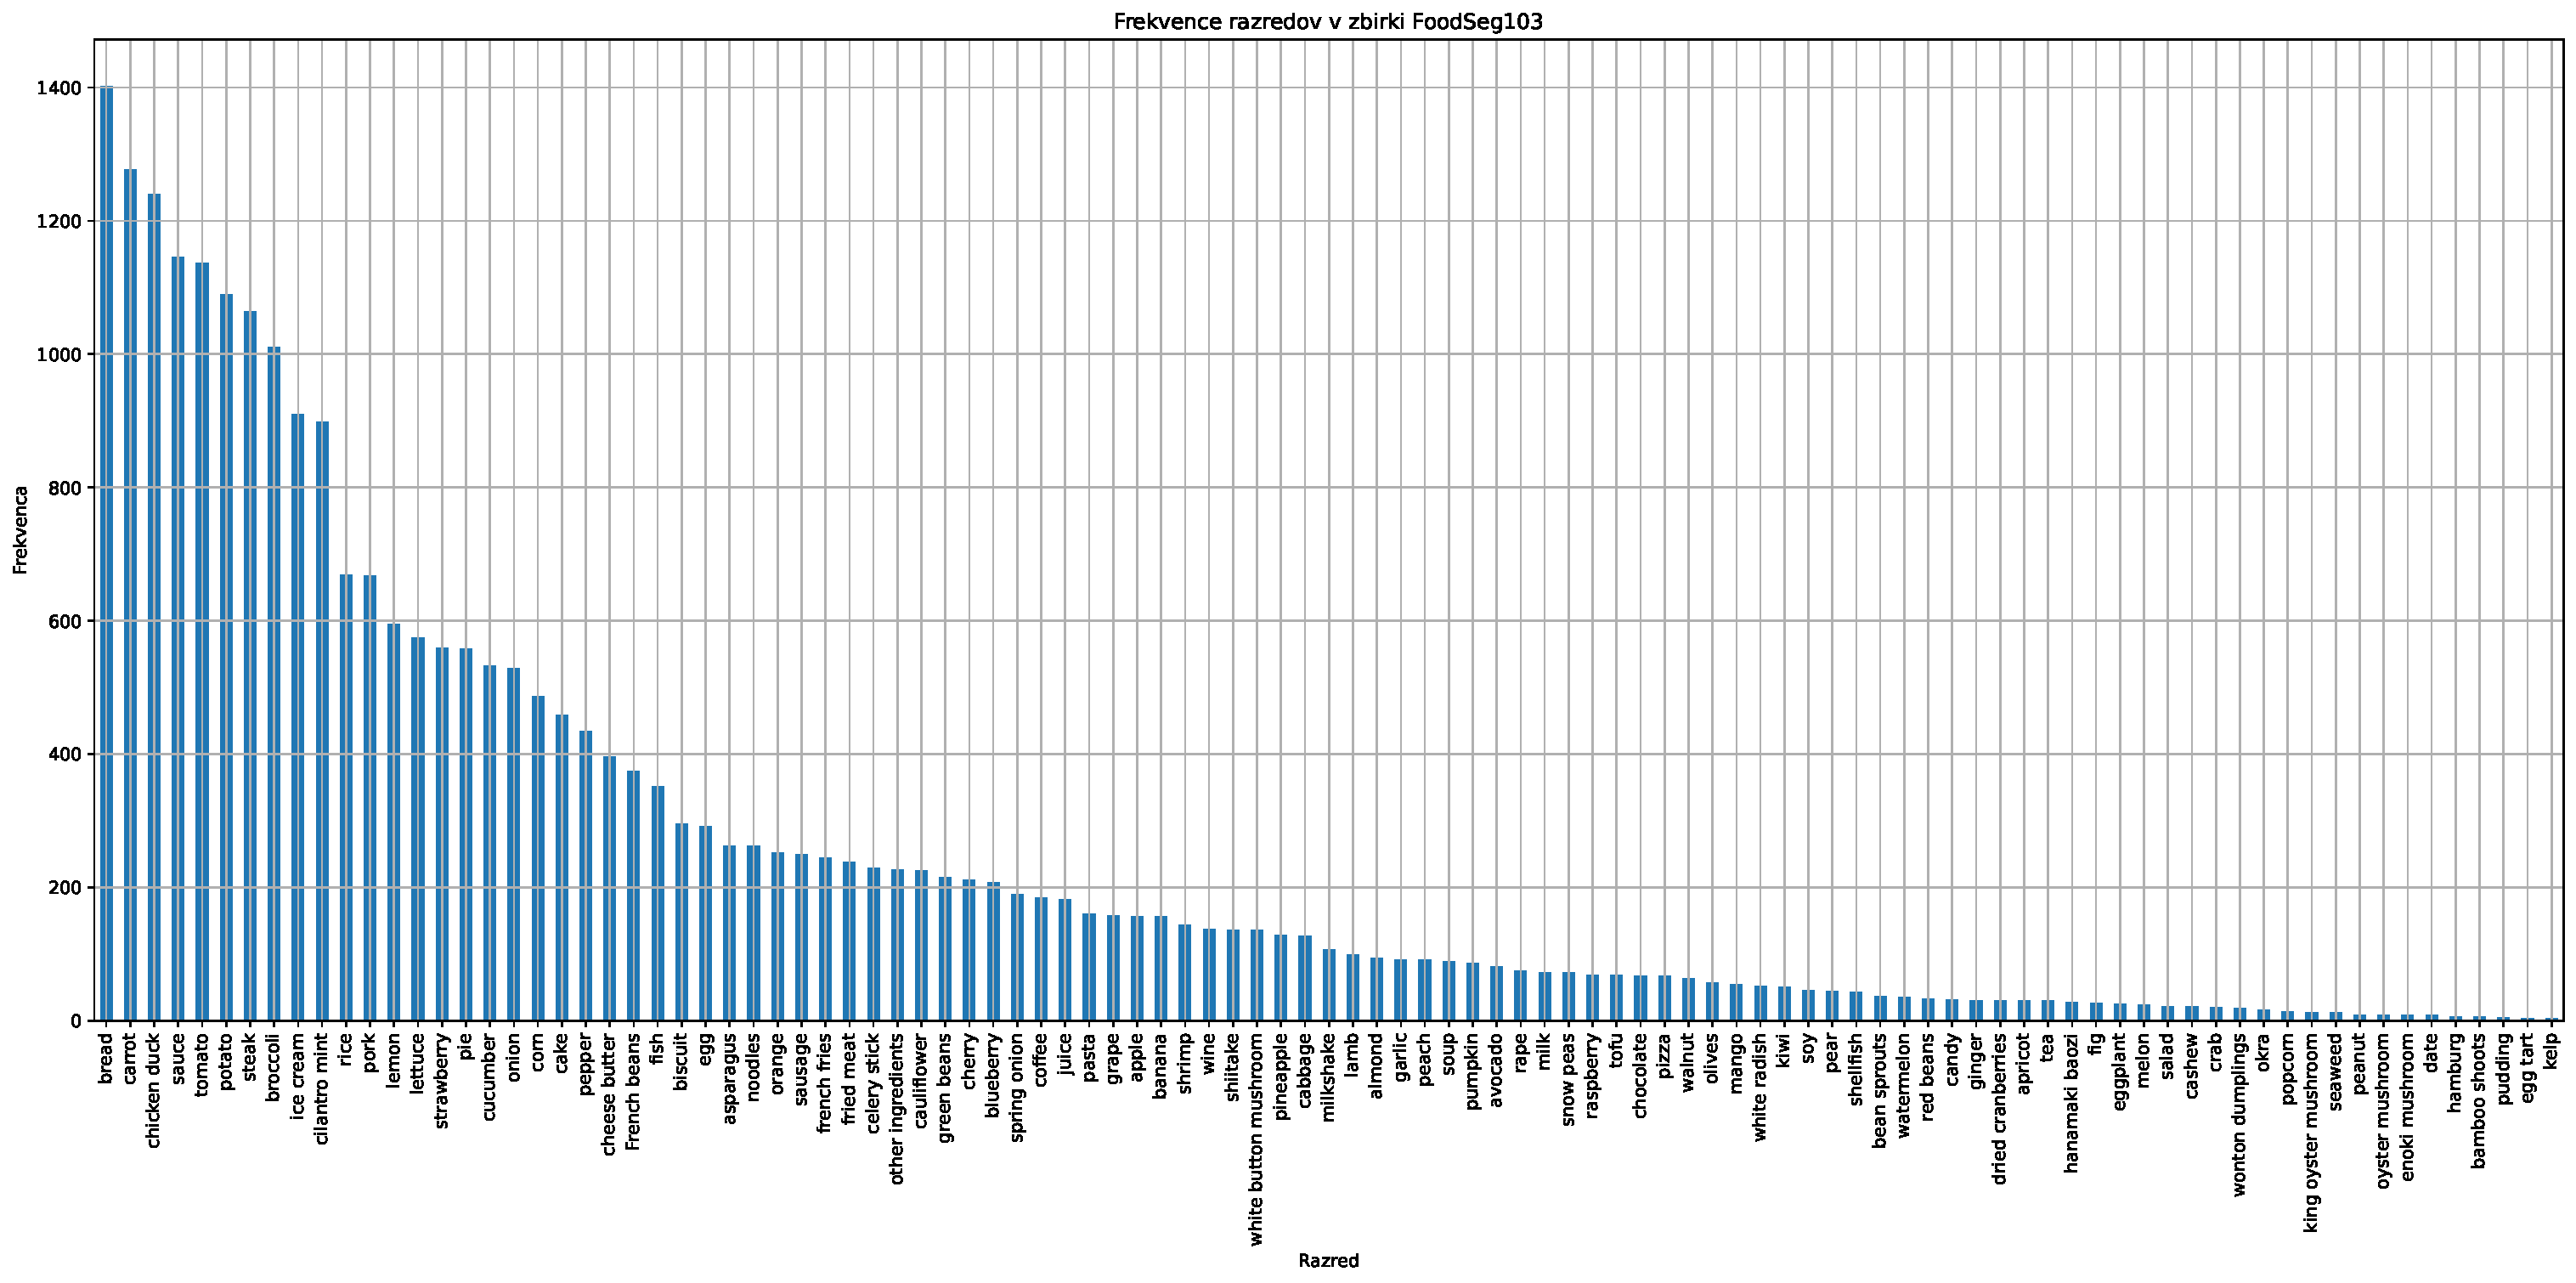
\includegraphics[height=250pt]{figures/class_frequencies_hist.pdf}
                % TODO: Dodaj opis slike
                %\caption{}
                \label{fig:foodseg103_orig_distribution}
            \end{turn}

\end{document}
%%%%%%%%%%%%%%%%%%%%%%%%%%%%%%%%%%%%%%%%%%%%%%%%%%%%%%%%%%%%%%%%%%%%%%%%%%%%%%%%%%%%%%%%%%%%%%%%%%%%%%%%%%%%%%%%%%%%%%%%
